\documentclass[twoside]{book}

% Packages required by doxygen
\usepackage{fixltx2e}
\usepackage{calc}
\usepackage{doxygen}
\usepackage[export]{adjustbox} % also loads graphicx
\usepackage{graphicx}
\usepackage[utf8]{inputenc}
\usepackage{makeidx}
\usepackage{multicol}
\usepackage{multirow}
\PassOptionsToPackage{warn}{textcomp}
\usepackage{textcomp}
\usepackage[nointegrals]{wasysym}
\usepackage[table]{xcolor}

% Font selection
\usepackage[T1]{fontenc}
\usepackage[scaled=.90]{helvet}
\usepackage{courier}
\usepackage{amssymb}
\usepackage{sectsty}
\renewcommand{\familydefault}{\sfdefault}
\allsectionsfont{%
  \fontseries{bc}\selectfont%
  \color{darkgray}%
}
\renewcommand{\DoxyLabelFont}{%
  \fontseries{bc}\selectfont%
  \color{darkgray}%
}
\newcommand{\+}{\discretionary{\mbox{\scriptsize$\hookleftarrow$}}{}{}}

% Page & text layout
\usepackage{geometry}
\geometry{%
  a4paper,%
  top=2.5cm,%
  bottom=2.5cm,%
  left=2.5cm,%
  right=2.5cm%
}
\tolerance=750
\hfuzz=15pt
\hbadness=750
\setlength{\emergencystretch}{15pt}
\setlength{\parindent}{0cm}
\setlength{\parskip}{3ex plus 2ex minus 2ex}
\makeatletter
\renewcommand{\paragraph}{%
  \@startsection{paragraph}{4}{0ex}{-1.0ex}{1.0ex}{%
    \normalfont\normalsize\bfseries\SS@parafont%
  }%
}
\renewcommand{\subparagraph}{%
  \@startsection{subparagraph}{5}{0ex}{-1.0ex}{1.0ex}{%
    \normalfont\normalsize\bfseries\SS@subparafont%
  }%
}
\makeatother

% Headers & footers
\usepackage{fancyhdr}
\pagestyle{fancyplain}
\fancyhead[LE]{\fancyplain{}{\bfseries\thepage}}
\fancyhead[CE]{\fancyplain{}{}}
\fancyhead[RE]{\fancyplain{}{\bfseries\leftmark}}
\fancyhead[LO]{\fancyplain{}{\bfseries\rightmark}}
\fancyhead[CO]{\fancyplain{}{}}
\fancyhead[RO]{\fancyplain{}{\bfseries\thepage}}
\fancyfoot[LE]{\fancyplain{}{}}
\fancyfoot[CE]{\fancyplain{}{}}
\fancyfoot[RE]{\fancyplain{}{\bfseries\scriptsize Generated by Doxygen }}
\fancyfoot[LO]{\fancyplain{}{\bfseries\scriptsize Generated by Doxygen }}
\fancyfoot[CO]{\fancyplain{}{}}
\fancyfoot[RO]{\fancyplain{}{}}
\renewcommand{\footrulewidth}{0.4pt}
\renewcommand{\chaptermark}[1]{%
  \markboth{#1}{}%
}
\renewcommand{\sectionmark}[1]{%
  \markright{\thesection\ #1}%
}

% Indices & bibliography
\usepackage{natbib}
\usepackage[titles]{tocloft}
\setcounter{tocdepth}{3}
\setcounter{secnumdepth}{5}
\makeindex

% Hyperlinks (required, but should be loaded last)
\usepackage{ifpdf}
\ifpdf
  \usepackage[pdftex,pagebackref=true]{hyperref}
\else
  \usepackage[ps2pdf,pagebackref=true]{hyperref}
\fi
\hypersetup{%
  colorlinks=true,%
  linkcolor=blue,%
  citecolor=blue,%
  unicode%
}

% Custom commands
\newcommand{\clearemptydoublepage}{%
  \newpage{\pagestyle{empty}\cleardoublepage}%
}

\usepackage{caption}
\captionsetup{labelsep=space,justification=centering,font={bf},singlelinecheck=off,skip=4pt,position=top}

%===== C O N T E N T S =====

\begin{document}

% Titlepage & ToC
\hypersetup{pageanchor=false,
             bookmarksnumbered=true,
             pdfencoding=unicode
            }
\pagenumbering{alph}
\begin{titlepage}
\vspace*{7cm}
\begin{center}%
{\Large Intel H\+E\+XL }\\
\vspace*{1cm}
{\large Generated by Doxygen 1.8.13}\\
\end{center}
\end{titlepage}
\clearemptydoublepage
\pagenumbering{roman}
\tableofcontents
\clearemptydoublepage
\pagenumbering{arabic}
\hypersetup{pageanchor=true}

%--- Begin generated contents ---
\chapter{Intel Homomorphic Encryption Acceleration Library (H\+E\+XL)}
\label{index}\hypertarget{index}{}\href{https://github.com/intel/hexl/actions/workflows/github-ci.yml}{\texttt{ }}\hypertarget{index_autotoc_md0}{}\doxysection{Intel Homomorphic Encryption Acceleration Library (\+H\+E\+X\+L)}\label{index_autotoc_md0}
Intel\+:registered\+: H\+E\+XL is an open-\/source library which provides efficient implementations of integer arithmetic on Galois fields. Such arithmetic is prevalent in cryptography, particularly in homomorphic encryption (HE) schemes. Intel H\+E\+XL targets integer arithmetic with word-\/sized primes, typically 30-\/60 bits. Intel H\+E\+XL provides an A\+PI for 64-\/bit unsigned integers and targets Intel C\+P\+Us. For more details on Intel H\+E\+XL, see our \href{https://arxiv.org/abs/2103.16400.pdf}{\texttt{ whitepaper}}. For tips on best performance, see \href{\#performance}{\texttt{ Performance}}\hypertarget{index_autotoc_md1}{}\doxysubsection{Contents}\label{index_autotoc_md1}

\begin{DoxyItemize}
\item \href{\#intel-homomorphic-encryption-acceleration-library-hexl}{\texttt{ Intel Homomorphic Encryption Acceleration Library (H\+E\+XL)}}
\begin{DoxyItemize}
\item \href{\#contents}{\texttt{ Contents}}
\item \href{\#introduction}{\texttt{ Introduction}}
\item \href{\#building-intel-hexl}{\texttt{ Building Intel H\+E\+XL}}
\begin{DoxyItemize}
\item \href{\#dependencies}{\texttt{ Dependencies}}
\item \href{\#compile-time-options}{\texttt{ Compile-\/time options}}
\item \href{\#compiling-intel-hexl}{\texttt{ Compiling Intel H\+E\+XL}}
\begin{DoxyItemize}
\item \href{\#linux-and-mac}{\texttt{ Linux and Mac}}
\item \href{\#windows}{\texttt{ Windows}}
\end{DoxyItemize}
\end{DoxyItemize}
\item \href{\#performance}{\texttt{ Performance}}
\item \href{\#testing-intel-hexl}{\texttt{ Testing Intel H\+E\+XL}}
\item \href{\#benchmarking-intel-hexl}{\texttt{ Benchmarking Intel H\+E\+XL}}
\item \href{\#using-intel-hexl}{\texttt{ Using Intel H\+E\+XL}}
\item \href{\#debugging}{\texttt{ Debugging}}
\item \href{\#threading}{\texttt{ Threading}}
\end{DoxyItemize}
\item \href{\#community-adoption}{\texttt{ Community Adoption}}
\item \href{\#documentation}{\texttt{ Documentation}}
\item \href{\#contributing}{\texttt{ Contributing}}
\begin{DoxyItemize}
\item \href{\#repository-layout}{\texttt{ Repository layout}}
\end{DoxyItemize}
\item \href{\#citing-intel-hexl}{\texttt{ Citing Intel H\+E\+XL}}
\begin{DoxyItemize}
\item \href{\#version-12}{\texttt{ Version 1.\+2}}
\item \href{\#version-11}{\texttt{ Version 1.\+1}}
\item \href{\#version-10}{\texttt{ Version 1.\+0}}
\end{DoxyItemize}
\item \href{\#contributors}{\texttt{ Contributors}}
\end{DoxyItemize}\hypertarget{index_autotoc_md2}{}\doxysubsection{Introduction}\label{index_autotoc_md2}
Many cryptographic applications, particularly homomorphic encryption (HE), rely on integer polynomial arithmetic in a finite field. HE, which enables computation on encrypted data, typically uses polynomials with degree {\ttfamily N} a power of two roughly in the range {\ttfamily N=\mbox{[}2$^\wedge$\{10\}, 2$^\wedge$\{17\}\mbox{]}}. The coefficients of these polynomials are in a finite field with a word-\/sized prime, {\ttfamily q}, up to {\ttfamily q}$\sim$62 bits. More precisely, the polynomials live in the ring {\ttfamily Z\+\_\+q\mbox{[}X\mbox{]}/(X$^\wedge$N + 1)}. That is, when adding or multiplying two polynomials, each coefficient of the result is reduced by the prime modulus {\ttfamily q}. When multiplying two polynomials, the resulting polynomials of degree {\ttfamily 2N} is additionally reduced by taking the remainder when dividing by {\ttfamily X$^\wedge$\+N+1}.

The primary bottleneck in many HE applications is polynomial-\/polynomial multiplication in {\ttfamily Z\+\_\+q\mbox{[}X\mbox{]}/(X$^\wedge$N + 1)}. For efficient implementation, Intel H\+E\+XL implements the negacyclic number-\/theoretic transform (N\+TT). To multiply two polynomials, {\ttfamily q\+\_\+1(x), q\+\_\+2(x)} using the N\+TT, we perform the Fwd\+N\+TT on the two input polynomials, then perform an element-\/wise modular multiplication, and perform the Inv\+N\+TT on the result.

Intel H\+E\+XL implements the following functions\+:
\begin{DoxyItemize}
\item The forward and inverse negacyclic number-\/theoretic transform (N\+TT)
\item Element-\/wise vector-\/vector modular multiplication
\item Element-\/wise vector-\/scalar modular multiplication with optional addition
\item Element-\/wise modular multiplication
\end{DoxyItemize}

For each function, the library implements one or several Intel(\+R) A\+V\+X-\/512 implementations, as well as a less performant, more readable native C++ implementation. Intel H\+E\+XL will automatically choose the best implementation for the given C\+PU Intel(\+R) A\+V\+X-\/512 feature set. In particular, when the modulus {\ttfamily q} is less than {\ttfamily 2$^\wedge$\{50\}}, the A\+V\+X512\+I\+F\+MA instruction set available on Intel Ice\+Lake server and Ice\+Lake client will provide a more efficient implementation.

For additional functionality, see the public headers, located in {\ttfamily include/hexl}\hypertarget{index_autotoc_md3}{}\doxysubsection{Building Intel H\+E\+XL}\label{index_autotoc_md3}
Intel H\+E\+XL can be built in several ways. Intel H\+E\+XL has been uploaded to the \href{https://github.com/microsoft/vcpkg}{\texttt{ Microsoft vcpkg}} C++ package manager, which supports Linux, mac\+OS, and Windows builds. See the vcpkg repository for instructions to build Intel H\+E\+XL with vcpkg, e.\+g. run {\ttfamily vcpkg install hexl}. There may be some delay in uploading latest release ports to vcpkg. Intel H\+E\+XL provides port files to build the latest version with vcpkg. For a static build, run {\ttfamily vcpkg install hexl -\/-\/overlay-\/ports=/path/to/hexl/port/hexl -\/-\/head}. For dynamic build, use the custom triplet file and run {\ttfamily vcpkg install hexl\+:hexl-\/dynamic-\/build -\/-\/overlay-\/ports=/path/to/hexl/port/hexl -\/-\/head -\/-\/overlay-\/triplets=/path/to/hexl/port/hexl}. For detailed explanation, see \href{https://devblogs.microsoft.com/cppblog/registries-bring-your-own-libraries-to-vcpkg/}{\texttt{ instruction}} for building vcpkg port using overlays and use of \href{https://github.com/microsoft/vcpkg/blob/master/docs/examples/overlay-triplets-linux-dynamic.md\#building-dynamic-libraries-on-linux}{\texttt{ custom triplet}} provided by vcpkg.

Intel H\+E\+XL also supports a build using the C\+Make build system. See below for the instructions to build Intel H\+E\+XL from source using C\+Make.\hypertarget{index_autotoc_md4}{}\doxysubsubsection{Dependencies}\label{index_autotoc_md4}
We have tested Intel H\+E\+XL on the following operating systems\+:
\begin{DoxyItemize}
\item Ubuntu 20.\+04
\item mac\+OS 10.\+15
\item Microsoft Windows 10
\end{DoxyItemize}

Intel H\+E\+XL requires the following dependencies\+:

\tabulinesep=1mm
\begin{longtabu}spread 0pt [c]{*{2}{|X[-1]}|}
\hline
\PBS\centering \cellcolor{\tableheadbgcolor}\textbf{ Dependency }&\PBS\centering \cellcolor{\tableheadbgcolor}\textbf{ Version  }\\\cline{1-2}
\endfirsthead
\hline
\endfoot
\hline
\PBS\centering \cellcolor{\tableheadbgcolor}\textbf{ Dependency }&\PBS\centering \cellcolor{\tableheadbgcolor}\textbf{ Version  }\\\cline{1-2}
\endhead
C\+Make &$>$= 3.\+5.\+1  \\\cline{1-2}
Compiler &gcc $>$= 7.\+0, clang++ $>$= 5.\+0, M\+S\+VC $>$= 2019  \\\cline{1-2}
\end{longtabu}
\hypertarget{index_autotoc_md5}{}\doxysubsubsection{Compile-\/time options}\label{index_autotoc_md5}
In addition to the standard C\+Make build options, Intel H\+E\+XL supports several compile-\/time flags to configure the build. For convenience, they are listed below\+:

\tabulinesep=1mm
\begin{longtabu}spread 0pt [c]{*{4}{|X[-1]}|}
\hline
\PBS\centering \cellcolor{\tableheadbgcolor}\textbf{ C\+Make option }&\PBS\centering \cellcolor{\tableheadbgcolor}\textbf{ Values }&\PBS\centering \cellcolor{\tableheadbgcolor}\textbf{ Default }&\PBS\centering \cellcolor{\tableheadbgcolor}\textbf{ }\\\cline{1-4}
\endfirsthead
\hline
\endfoot
\hline
\PBS\centering \cellcolor{\tableheadbgcolor}\textbf{ C\+Make option }&\PBS\centering \cellcolor{\tableheadbgcolor}\textbf{ Values }&\PBS\centering \cellcolor{\tableheadbgcolor}\textbf{ Default }&\PBS\centering \cellcolor{\tableheadbgcolor}\textbf{ }\\\cline{1-4}
\endhead
H\+E\+X\+L\+\_\+\+B\+E\+N\+C\+H\+M\+A\+RK &ON / O\+FF &ON &Set to ON to enable benchmark suite via Google benchmark  \\\cline{1-4}
H\+E\+X\+L\+\_\+\+C\+O\+V\+E\+R\+A\+GE &ON / O\+FF &O\+FF &Set to ON to enable coverage report of unit-\/tests  \\\cline{1-4}
H\+E\+X\+L\+\_\+\+S\+H\+A\+R\+E\+D\+\_\+\+L\+IB &ON / O\+FF &O\+FF &Set to ON to enable building shared library  \\\cline{1-4}
H\+E\+X\+L\+\_\+\+D\+O\+CS &ON / O\+FF &O\+FF &Set to ON to enable building of documentation  \\\cline{1-4}
H\+E\+X\+L\+\_\+\+T\+E\+S\+T\+I\+NG &ON / O\+FF &ON &Set to ON to enable building of unit-\/tests  \\\cline{1-4}
H\+E\+X\+L\+\_\+\+T\+R\+E\+A\+T\+\_\+\+W\+A\+R\+N\+I\+N\+G\+\_\+\+A\+S\+\_\+\+E\+R\+R\+OR &ON / O\+FF &O\+FF &Set to ON to treat all warnings as error  \\\cline{1-4}
\end{longtabu}
\hypertarget{index_autotoc_md6}{}\doxysubsubsection{Compiling Intel H\+E\+XL}\label{index_autotoc_md6}
To compile Intel H\+E\+XL from source code, first clone the repository and change directories to the where the source has been cloned. \hypertarget{index_autotoc_md7}{}\doxyparagraph{Linux and Mac}\label{index_autotoc_md7}
The instructions to build Intel H\+E\+XL are common to Linux and Mac\+OS.

Then, to configure the build, call 
\begin{DoxyCode}{0}
\DoxyCodeLine{cmake -\/S . -\/B build}
\end{DoxyCode}


adding the desired compile-\/time options with a {\ttfamily -\/D} flag. For instance, to build Intel H\+E\+XL as a shared library, call 
\begin{DoxyCode}{0}
\DoxyCodeLine{cmake -\/S . -\/B build -\/DHEXL\_SHARED\_LIB=ON}
\end{DoxyCode}


Then, to build Intel H\+E\+XL, call 
\begin{DoxyCode}{0}
\DoxyCodeLine{cmake -\/-\/build build}
\end{DoxyCode}


This will build the Intel H\+E\+XL library in the {\ttfamily build/hexl/lib/} directory.

To install Intel H\+E\+XL to the installation directory, run 
\begin{DoxyCode}{0}
\DoxyCodeLine{cmake -\/-\/install build}
\end{DoxyCode}


To use a non-\/standard installation directory, configure the build with 
\begin{DoxyCode}{0}
\DoxyCodeLine{cmake -\/S . -\/B build -\/DCMAKE\_INSTALL\_PREFIX=/path/to/install}
\end{DoxyCode}


before proceeding with the build and installation directions above.\hypertarget{index_autotoc_md8}{}\doxyparagraph{Windows}\label{index_autotoc_md8}
To compile Intel H\+E\+XL on Windows using Visual Studio in Release mode, configure the build via 
\begin{DoxyCode}{0}
\DoxyCodeLine{cmake -\/S . -\/B build -\/G "Visual Studio 16 2019" -\/DCMAKE\_BUILD\_TYPE=Release}
\end{DoxyCode}


adding the desired compile-\/time options with a {\ttfamily -\/D} flag (see \href{\#compile-time-options}{\texttt{ Compile-\/time options}}).

To specify the desired build configuration, pass either {\ttfamily -\/-\/config Debug} or {\ttfamily -\/-\/config Release} to the build step and install steps. For instance, to build Intel H\+E\+XL in Release mode, call 
\begin{DoxyCode}{0}
\DoxyCodeLine{cmake -\/-\/build build -\/-\/config Release}
\end{DoxyCode}


This will build the Intel H\+E\+XL library in the {\ttfamily build/hexl/lib/} or {\ttfamily build/hexl/\+Release/lib} directory.

To install Intel H\+E\+XL to the installation directory, run 
\begin{DoxyCode}{0}
\DoxyCodeLine{cmake -\/-\/build build -\/-\/target install -\/-\/config Release}
\end{DoxyCode}


To use a non-\/standard installation directory, configure the build with 
\begin{DoxyCode}{0}
\DoxyCodeLine{cmake -\/S . -\/B build -\/G "Visual Studio 16 2019" -\/DCMAKE\_BUILD\_TYPE=Release -\/DCMAKE\_INSTALL\_PREFIX=/path/to/install}
\end{DoxyCode}


before proceeding with the build and installation directions above.\hypertarget{index_autotoc_md9}{}\doxysubsection{Performance}\label{index_autotoc_md9}
For best performance, we recommend using Intel H\+E\+XL on a Linux system with the clang++-\/12 compiler. We also recommend using a processor with Intel A\+V\+X512\+DQ support, with best performance on processors supporting Intel A\+V\+X512-\/\+I\+F\+M\+A52. To determine if your processor supports A\+V\+X512-\/\+I\+F\+M\+A52, simply look for {\ttfamily -\/-\/ Setting H\+E\+X\+L\+\_\+\+H\+A\+S\+\_\+\+A\+V\+X512\+I\+F\+MA} printed during the configure step.

See the below table for setting the modulus {\ttfamily q} for best performance. \tabulinesep=1mm
\begin{longtabu}spread 0pt [c]{*{2}{|X[-1]}|}
\hline
\PBS\centering \cellcolor{\tableheadbgcolor}\textbf{ Instruction Set }&\PBS\centering \cellcolor{\tableheadbgcolor}\textbf{ Bound on modulus {\ttfamily q}  }\\\cline{1-2}
\endfirsthead
\hline
\endfoot
\hline
\PBS\centering \cellcolor{\tableheadbgcolor}\textbf{ Instruction Set }&\PBS\centering \cellcolor{\tableheadbgcolor}\textbf{ Bound on modulus {\ttfamily q}  }\\\cline{1-2}
\endhead
A\+V\+X512-\/\+DQ &{\ttfamily q $<$ 2$^\wedge$30}  \\\cline{1-2}
A\+V\+X512-\/\+I\+F\+M\+A52 &{\ttfamily q $<$ 2$^\wedge$50}  \\\cline{1-2}
\end{longtabu}


Some speedup is still expected for moduli {\ttfamily q $>$ 2$^\wedge$30} using the A\+V\+X512-\/\+DQ instruction set.\hypertarget{index_autotoc_md10}{}\doxysubsection{Testing Intel H\+E\+XL}\label{index_autotoc_md10}
To run a set of unit tests via \href{https://github.com/google/googletest}{\texttt{ Googletest}}, configure and build Intel H\+E\+XL with {\ttfamily -\/D\+H\+E\+X\+L\+\_\+\+T\+E\+S\+T\+I\+NG=ON} (see \href{\#compile-time-options}{\texttt{ Compile-\/time options}}). Then, run 
\begin{DoxyCode}{0}
\DoxyCodeLine{cmake -\/-\/build build -\/-\/target unittest}
\end{DoxyCode}


The unit-\/test executable itself is located at {\ttfamily build/test/unit-\/test} on Linux and Mac, and at {\ttfamily build\textbackslash{}test\textbackslash{}Release\textbackslash{}unit-\/test.\+exe} or {\ttfamily build\textbackslash{}test\textbackslash{}Debug\textbackslash{}unit-\/test.\+exe} on Windows. \hypertarget{index_autotoc_md11}{}\doxysubsection{Benchmarking Intel H\+E\+XL}\label{index_autotoc_md11}
To run a set of benchmarks via \href{https://github.com/google/benchmark}{\texttt{ Google benchmark}}, configure and build Intel H\+E\+XL with {\ttfamily -\/D\+H\+E\+X\+L\+\_\+\+B\+E\+N\+C\+H\+M\+A\+RK=ON} (see \href{\#compile-time-options}{\texttt{ Compile-\/time options}}). Then, run 
\begin{DoxyCode}{0}
\DoxyCodeLine{cmake -\/-\/build build -\/-\/target bench}
\end{DoxyCode}


On Windows, run 
\begin{DoxyCode}{0}
\DoxyCodeLine{cmake -\/-\/build build -\/-\/target bench -\/-\/config Release}
\end{DoxyCode}


The benchmark executable itself is located at {\ttfamily build/benchmark/bench\+\_\+hexl} on Linux and Mac, and at {\ttfamily build\textbackslash{}benchmark\textbackslash{}Debug\textbackslash{}bench\+\_\+hexl.\+exe} or {\ttfamily build\textbackslash{}benchmark\textbackslash{}Release\textbackslash{}bench\+\_\+hexl.\+exe} on Windows.\hypertarget{index_autotoc_md12}{}\doxysubsection{Using Intel H\+E\+XL}\label{index_autotoc_md12}
The {\ttfamily example} folder has an example of using Intel H\+E\+XL in a third-\/party project.\hypertarget{index_autotoc_md13}{}\doxysubsection{Debugging}\label{index_autotoc_md13}
For optimal performance, Intel H\+E\+XL does not perform input validation. In many cases the time required for the validation would be longer than the execution of the function itself. To debug Intel H\+E\+XL, configure and build Intel H\+E\+XL with {\ttfamily -\/D\+C\+M\+A\+K\+E\+\_\+\+B\+U\+I\+L\+D\+\_\+\+T\+Y\+PE=Debug} (see \href{\#compile-time-options}{\texttt{ Compile-\/time options}}). This will generate a debug version of the library, e.\+g. {\ttfamily libhexl\+\_\+debug.\+a}, that can be used to debug the execution. In Debug mode, Intel H\+E\+XL will also link against \href{https://github.com/google/sanitizers/wiki/AddressSanitizer}{\texttt{ Address Sanitizer}}.

{\bfseries{Note}}, enabling {\ttfamily C\+M\+A\+K\+E\+\_\+\+B\+U\+I\+L\+D\+\_\+\+T\+Y\+PE=Debug} will result in a significant runtime overhead.

To enable verbose logging for the benchmarks or unit-\/tests in a Debug build, add the log level as a command-\/line argument, e.\+g. {\ttfamily build/benchmark/bench\+\_\+hexl -\/-\/v=9}. See \href{https://github.com/amrayn/easyloggingpp\#application-arguments}{\texttt{ easyloggingpp\textquotesingle{}s documentation}} for more details.\hypertarget{index_autotoc_md14}{}\doxysubsection{Threading}\label{index_autotoc_md14}
Intel H\+E\+XL is single-\/threaded and thread-\/safe.\hypertarget{index_autotoc_md15}{}\doxysection{Community Adoption}\label{index_autotoc_md15}
Intel H\+E\+XL has been integrated to the following homomorphic encryption libraries\+:
\begin{DoxyItemize}
\item \href{https://github.com/homenc/HElib}{\texttt{ H\+Elib}}
\item \href{https://github.com/microsoft/SEAL}{\texttt{ Microsoft S\+E\+AL}}
\item \href{https://gitlab.com/palisade/palisade-release}{\texttt{ P\+A\+L\+I\+S\+A\+DE}}
\end{DoxyItemize}

See also the \href{https://github.com/intel/he-toolkit}{\texttt{ Intel Homomorphic Encryption Toolkit}} for example uses cases using H\+E\+XL.

Please let us know if you are aware of any other uses of Intel H\+E\+XL.\hypertarget{index_autotoc_md16}{}\doxysection{Documentation}\label{index_autotoc_md16}
Intel H\+E\+XL supports documentation via Doxygen. See \href{https://intel.github.io/hexl}{\texttt{ https\+://intel.\+github.\+io/hexl}} for the latest Doxygen documentation.

To build documentation, first install {\ttfamily doxygen} and {\ttfamily graphviz}, e.\+g. 
\begin{DoxyCode}{0}
\DoxyCodeLine{sudo apt-\/get install doxygen graphviz}
\end{DoxyCode}


Then, configure Intel H\+E\+XL with {\ttfamily -\/D\+H\+E\+X\+L\+\_\+\+D\+O\+CS=ON} (see \href{\#compile-time-options}{\texttt{ Compile-\/time options}}). To build Doxygen documentation, after configuring Intel H\+E\+XL with {\ttfamily -\/D\+H\+E\+X\+L\+\_\+\+D\+O\+CS=ON}, run 
\begin{DoxyCode}{0}
\DoxyCodeLine{cmake -\/-\/build build -\/-\/target docs}
\end{DoxyCode}


To view the generated Doxygen documentation, open the generated {\ttfamily docs/doxygen/html/index.\+html} file in a web browser.\hypertarget{index_autotoc_md17}{}\doxysection{Contributing}\label{index_autotoc_md17}
This project welcomes external contributions. To contribute to Intel H\+E\+XL, see \mbox{\hyperlink{CONTRIBUTING_8md}{C\+O\+N\+T\+R\+I\+B\+U\+T\+I\+NG.md}}. We encourage feedback and suggestions via \href{https://github.com/intel/hexl/issues}{\texttt{ Github Issues}} as well as discussion via \href{https://github.com/intel/hexl/discussions}{\texttt{ Github Discussions}}.\hypertarget{index_autotoc_md18}{}\doxysubsection{Repository layout}\label{index_autotoc_md18}
Public headers reside in the {\ttfamily hexl/include} folder. Private headers, e.\+g. those containing Intel(\+R) A\+V\+X-\/512 code should not be put in this folder.\hypertarget{index_autotoc_md19}{}\doxysection{Citing Intel H\+E\+XL}\label{index_autotoc_md19}
To cite Intel H\+E\+XL, please use the following Bib\+TeX entry.\hypertarget{index_autotoc_md20}{}\doxysubsubsection{Version 1.\+2}\label{index_autotoc_md20}

\begin{DoxyCode}{0}
\DoxyCodeLine{@misc\{IntelHEXL,}
\DoxyCodeLine{    author=\{Boemer, Fabian and Kim, Sejun and Seifu, Gelila and de Souza, Fillipe DM and Gopal, Vinodh and others\},}
\DoxyCodeLine{    title = \{\{I\}ntel \{HEXL\} (release 1.2)\},}
\DoxyCodeLine{    howpublished = \{\(\backslash\)url\{https://github.com/intel/hexl\}\},}
\DoxyCodeLine{    month = september,}
\DoxyCodeLine{    year = 2021,}
\DoxyCodeLine{    key = \{Intel HEXL\}}
\DoxyCodeLine{\}}
\end{DoxyCode}
\hypertarget{index_autotoc_md21}{}\doxysubsubsection{Version 1.\+1}\label{index_autotoc_md21}

\begin{DoxyCode}{0}
\DoxyCodeLine{@misc\{IntelHEXL,}
\DoxyCodeLine{    author=\{Boemer, Fabian and Kim, Sejun and Seifu, Gelila and de Souza, Fillipe DM and Gopal, Vinodh and others\},}
\DoxyCodeLine{    title = \{\{I\}ntel \{HEXL\} (release 1.1)\},}
\DoxyCodeLine{    howpublished = \{\(\backslash\)url\{https://github.com/intel/hexl\}\},}
\DoxyCodeLine{    month = may,}
\DoxyCodeLine{    year = 2021,}
\DoxyCodeLine{    key = \{Intel HEXL\}}
\DoxyCodeLine{\}}
\end{DoxyCode}
\hypertarget{index_autotoc_md22}{}\doxysubsubsection{Version 1.\+0}\label{index_autotoc_md22}

\begin{DoxyCode}{0}
\DoxyCodeLine{@misc\{IntelHEXL,}
\DoxyCodeLine{    author=\{Boemer, Fabian and Kim, Sejun and Seifu, Gelila and de Souza, Fillipe DM and Gopal, Vinodh and others\},}
\DoxyCodeLine{    title = \{\{I\}ntel \{HEXL\} (release 1.0)\},}
\DoxyCodeLine{    howpublished = \{\(\backslash\)url\{https://github.com/intel/hexl\}\},}
\DoxyCodeLine{    month = april,}
\DoxyCodeLine{    year = 2021,}
\DoxyCodeLine{    key = \{Intel HEXL\}}
\DoxyCodeLine{\}}
\end{DoxyCode}
\hypertarget{index_autotoc_md23}{}\doxysection{Contributors}\label{index_autotoc_md23}
The Intel contributors to this project, sorted by last name, are
\begin{DoxyItemize}
\item \href{https://www.linkedin.com/in/paky-abu-alam-89797710/}{\texttt{ Paky Abu-\/\+Alam}}
\item \href{https://www.linkedin.com/in/flavio-bergamaschi-1634141/}{\texttt{ Flavio Bergamaschi}}
\item \href{https://www.linkedin.com/in/fabian-boemer-5a40a9102/}{\texttt{ Fabian Boemer}} (lead)
\item \href{https://www.linkedin.com/in/jeremy-bottleson-38852a7/}{\texttt{ Jeremy Bottleson}}
\item \href{https://www.linkedin.com/in/jacklhcrawford/}{\texttt{ Jack Crawford}}
\item \href{https://www.linkedin.com/in/fillipe-d-m-de-souza-a8281820/}{\texttt{ Fillipe D.\+M. de Souza}}
\item \href{https://www.linkedin.com/in/sergey-ivanov-451b72195/}{\texttt{ Sergey Ivanov}}
\item \href{https://www.linkedin.com/in/akshaya-jagannadharao/}{\texttt{ Akshaya Jagannadharao}}
\item \href{https://www.linkedin.com/in/jingyi-jin-655735/}{\texttt{ Jingyi Jin}}
\item \href{https://www.linkedin.com/in/sejun-kim-2b1b4866/}{\texttt{ Sejun Kim}}
\item \href{https://www.linkedin.com/in/nir-peled-4a52266/}{\texttt{ Nir Peled}}
\item \href{https://www.linkedin.com/in/kylanrace/}{\texttt{ Kylan Race}}
\item \href{https://www.linkedin.com/in/gelila-seifu/}{\texttt{ Gelila Seifu}}
\end{DoxyItemize}

In addition to the Intel contributors listed, we are also grateful to contributions to this project that are not reflected in the Git history\+:
\begin{DoxyItemize}
\item \href{https://www.linkedin.com/in/apapadimitriou/}{\texttt{ Antonis Papadimitriou}} 
\end{DoxyItemize}
\chapter{Pull Requests}
\label{md__home_gelila_Desktop_workspace_hexl_CONTRIBUTING}
\Hypertarget{md__home_gelila_Desktop_workspace_hexl_CONTRIBUTING}
Intel H\+E\+XL welcomes pull requests from external contributors.

Before contributing, please run 
\begin{DoxyCode}
cmake --build build --target check unittest
\end{DoxyCode}
 to make sure the formatting checks and all unit tests pass.

Please sign your commits before making a pull request. See instructions \href{https://docs.github.com/en/github/authenticating-to-github/managing-commit-signature-verification/signing-commits}{\tt here} for how to sign commits. 
\chapter{Namespace Index}
\doxysection{Namespace List}
Here is a list of all namespaces with brief descriptions\+:\begin{DoxyCompactList}
\item\contentsline{section}{\mbox{\hyperlink{namespaceintel}{intel}} }{\pageref{namespaceintel}}{}
\item\contentsline{section}{\mbox{\hyperlink{namespaceintel_1_1hexl}{intel\+::hexl}} }{\pageref{namespaceintel_1_1hexl}}{}
\end{DoxyCompactList}

\chapter{Hierarchical Index}
\section{Class Hierarchy}
This inheritance list is sorted roughly, but not completely, alphabetically\+:\begin{DoxyCompactList}
\item \contentsline{section}{intel\+:\+:hexl\+:\+:Aligned\+Allocator$<$ T, Alignment $>$}{\pageref{classintel_1_1hexl_1_1AlignedAllocator}}{}
\item \contentsline{section}{intel\+:\+:hexl\+:\+:Aligned\+Allocator$<$ uint64\+\_\+t, 64 $>$}{\pageref{classintel_1_1hexl_1_1AlignedAllocator}}{}
\item \contentsline{section}{intel\+:\+:hexl\+:\+:Allocator\+Base}{\pageref{structintel_1_1hexl_1_1AllocatorBase}}{}
\begin{DoxyCompactList}
\item \contentsline{section}{intel\+:\+:hexl\+:\+:Allocator\+Interface$<$ Allocator\+Adapter$<$ Adaptee, Args... $>$ $>$}{\pageref{structintel_1_1hexl_1_1AllocatorInterface}}{}
\begin{DoxyCompactList}
\item \contentsline{section}{intel\+:\+:hexl\+:\+:N\+TT\+:\+:Allocator\+Adapter$<$ Adaptee, Args $>$}{\pageref{structintel_1_1hexl_1_1NTT_1_1AllocatorAdapter}}{}
\end{DoxyCompactList}
\item \contentsline{section}{intel\+:\+:hexl\+:\+:Allocator\+Interface$<$ Allocator\+Impl $>$}{\pageref{structintel_1_1hexl_1_1AllocatorInterface}}{}
\item \contentsline{section}{intel\+:\+:hexl\+:\+:Malloc\+Strategy}{\pageref{structintel_1_1hexl_1_1MallocStrategy}}{}
\end{DoxyCompactList}
\item \contentsline{section}{intel\+:\+:hexl\+:\+:Multiply\+Factor}{\pageref{classintel_1_1hexl_1_1MultiplyFactor}}{}
\item \contentsline{section}{intel\+:\+:hexl\+:\+:N\+TT}{\pageref{classintel_1_1hexl_1_1NTT}}{}
\item \contentsline{section}{intel\+:\+:hexl\+:\+:Aligned\+Allocator$<$ T, Alignment $>$\+:\+:rebind$<$ U $>$}{\pageref{structintel_1_1hexl_1_1AlignedAllocator_1_1rebind}}{}
\end{DoxyCompactList}

\chapter{Class Index}
\section{Class List}
Here are the classes, structs, unions and interfaces with brief descriptions\+:\begin{DoxyCompactList}
\item\contentsline{section}{\hyperlink{classintel_1_1hexl_1_1AlignedAllocator}{intel\+::hexl\+::\+Aligned\+Allocator$<$ T, Alignment $>$} \\*Allocates memory aligned to Alignment-\/byte sized boundaries }{\pageref{classintel_1_1hexl_1_1AlignedAllocator}}{}
\item\contentsline{section}{\hyperlink{structintel_1_1hexl_1_1NTT_1_1AllocatorAdapter}{intel\+::hexl\+::\+N\+T\+T\+::\+Allocator\+Adapter$<$ Adaptee, Args $>$} \\*Helper class for custom memory allocation }{\pageref{structintel_1_1hexl_1_1NTT_1_1AllocatorAdapter}}{}
\item\contentsline{section}{\hyperlink{structintel_1_1hexl_1_1AllocatorBase}{intel\+::hexl\+::\+Allocator\+Base} \\*Base class for custom memory allocator }{\pageref{structintel_1_1hexl_1_1AllocatorBase}}{}
\item\contentsline{section}{\hyperlink{structintel_1_1hexl_1_1AllocatorInterface}{intel\+::hexl\+::\+Allocator\+Interface$<$ Allocator\+Impl $>$} \\*Helper memory allocation struct which delegates implementation to Allocator\+Impl }{\pageref{structintel_1_1hexl_1_1AllocatorInterface}}{}
\item\contentsline{section}{\hyperlink{structintel_1_1hexl_1_1MallocStrategy}{intel\+::hexl\+::\+Malloc\+Strategy} \\*Allocater implementation using malloc and free }{\pageref{structintel_1_1hexl_1_1MallocStrategy}}{}
\item\contentsline{section}{\hyperlink{classintel_1_1hexl_1_1MultiplyFactor}{intel\+::hexl\+::\+Multiply\+Factor} \\*Pre-\/computes a Barrett factor with which modular multiplication can be performed more efficiently }{\pageref{classintel_1_1hexl_1_1MultiplyFactor}}{}
\item\contentsline{section}{\hyperlink{classintel_1_1hexl_1_1NTT}{intel\+::hexl\+::\+N\+TT} \\*Performs negacyclic forward and inverse number-\/theoretic transform (\hyperlink{classintel_1_1hexl_1_1NTT}{N\+TT}), commonly used in R\+L\+WE cryptography }{\pageref{classintel_1_1hexl_1_1NTT}}{}
\item\contentsline{section}{\hyperlink{structintel_1_1hexl_1_1AlignedAllocator_1_1rebind}{intel\+::hexl\+::\+Aligned\+Allocator$<$ T, Alignment $>$\+::rebind$<$ U $>$} }{\pageref{structintel_1_1hexl_1_1AlignedAllocator_1_1rebind}}{}
\end{DoxyCompactList}

\chapter{File Index}
\doxysection{File List}
Here is a list of all files with brief descriptions\+:\begin{DoxyCompactList}
\item\contentsline{section}{\mbox{\hyperlink{aligned-allocator_8hpp}{aligned-\/allocator.\+hpp}} }{\pageref{aligned-allocator_8hpp}}{}
\item\contentsline{section}{\mbox{\hyperlink{allocator_8hpp}{allocator.\+hpp}} }{\pageref{allocator_8hpp}}{}
\item\contentsline{section}{\mbox{\hyperlink{check_8hpp}{check.\+hpp}} }{\pageref{check_8hpp}}{}
\item\contentsline{section}{\mbox{\hyperlink{ckks-multiply_8hpp}{ckks-\/multiply.\+hpp}} }{\pageref{ckks-multiply_8hpp}}{}
\item\contentsline{section}{\mbox{\hyperlink{ckks-switch-key_8hpp}{ckks-\/switch-\/key.\+hpp}} }{\pageref{ckks-switch-key_8hpp}}{}
\item\contentsline{section}{\mbox{\hyperlink{clang_8hpp}{clang.\+hpp}} }{\pageref{clang_8hpp}}{}
\item\contentsline{section}{\mbox{\hyperlink{compiler_8hpp}{compiler.\+hpp}} }{\pageref{compiler_8hpp}}{}
\item\contentsline{section}{\mbox{\hyperlink{defines_8hpp}{defines.\+hpp}} }{\pageref{defines_8hpp}}{}
\item\contentsline{section}{\mbox{\hyperlink{eltwise-add-mod_8hpp}{eltwise-\/add-\/mod.\+hpp}} }{\pageref{eltwise-add-mod_8hpp}}{}
\item\contentsline{section}{\mbox{\hyperlink{eltwise-cmp-add_8hpp}{eltwise-\/cmp-\/add.\+hpp}} }{\pageref{eltwise-cmp-add_8hpp}}{}
\item\contentsline{section}{\mbox{\hyperlink{eltwise-cmp-sub-mod_8hpp}{eltwise-\/cmp-\/sub-\/mod.\+hpp}} }{\pageref{eltwise-cmp-sub-mod_8hpp}}{}
\item\contentsline{section}{\mbox{\hyperlink{eltwise-fma-mod_8hpp}{eltwise-\/fma-\/mod.\+hpp}} }{\pageref{eltwise-fma-mod_8hpp}}{}
\item\contentsline{section}{\mbox{\hyperlink{eltwise-mult-mod_8hpp}{eltwise-\/mult-\/mod.\+hpp}} }{\pageref{eltwise-mult-mod_8hpp}}{}
\item\contentsline{section}{\mbox{\hyperlink{eltwise-reduce-mod_8hpp}{eltwise-\/reduce-\/mod.\+hpp}} }{\pageref{eltwise-reduce-mod_8hpp}}{}
\item\contentsline{section}{\mbox{\hyperlink{eltwise-sub-mod_8hpp}{eltwise-\/sub-\/mod.\+hpp}} }{\pageref{eltwise-sub-mod_8hpp}}{}
\item\contentsline{section}{\mbox{\hyperlink{gcc_8hpp}{gcc.\+hpp}} }{\pageref{gcc_8hpp}}{}
\item\contentsline{section}{\mbox{\hyperlink{hexl_8hpp}{hexl.\+hpp}} }{\pageref{hexl_8hpp}}{}
\item\contentsline{section}{\mbox{\hyperlink{logging_8hpp}{logging.\+hpp}} }{\pageref{logging_8hpp}}{}
\item\contentsline{section}{\mbox{\hyperlink{msvc_8hpp}{msvc.\+hpp}} }{\pageref{msvc_8hpp}}{}
\item\contentsline{section}{\mbox{\hyperlink{ntt_8hpp}{ntt.\+hpp}} }{\pageref{ntt_8hpp}}{}
\item\contentsline{section}{\mbox{\hyperlink{number-theory_8hpp}{number-\/theory.\+hpp}} }{\pageref{number-theory_8hpp}}{}
\item\contentsline{section}{\mbox{\hyperlink{types_8hpp}{types.\+hpp}} }{\pageref{types_8hpp}}{}
\item\contentsline{section}{\mbox{\hyperlink{util_8hpp}{util.\+hpp}} }{\pageref{util_8hpp}}{}
\end{DoxyCompactList}

\chapter{Namespace Documentation}
\hypertarget{namespaceintel}{}\section{intel Namespace Reference}
\label{namespaceintel}\index{intel@{intel}}
\subsection*{Namespaces}
\begin{DoxyCompactItemize}
\item 
 \hyperlink{namespaceintel_1_1hexl}{hexl}
\end{DoxyCompactItemize}

\hypertarget{namespaceintel_1_1hexl}{}\doxysection{intel\+::hexl Namespace Reference}
\label{namespaceintel_1_1hexl}\index{intel::hexl@{intel::hexl}}
\doxysubsection*{Classes}
\begin{DoxyCompactItemize}
\item 
class \mbox{\hyperlink{classintel_1_1hexl_1_1AlignedAllocator}{Aligned\+Allocator}}
\begin{DoxyCompactList}\small\item\em Allocates memory aligned to Alignment-\/byte sized boundaries. \end{DoxyCompactList}\item 
struct \mbox{\hyperlink{structintel_1_1hexl_1_1AllocatorBase}{Allocator\+Base}}
\begin{DoxyCompactList}\small\item\em Base class for custom memory allocator. \end{DoxyCompactList}\item 
struct \mbox{\hyperlink{structintel_1_1hexl_1_1AllocatorInterface}{Allocator\+Interface}}
\begin{DoxyCompactList}\small\item\em Helper memory allocation struct which delegates implementation to Allocator\+Impl. \end{DoxyCompactList}\item 
struct \mbox{\hyperlink{structintel_1_1hexl_1_1MallocStrategy}{Malloc\+Strategy}}
\begin{DoxyCompactList}\small\item\em Allocater implementation using malloc and free. \end{DoxyCompactList}\item 
class \mbox{\hyperlink{classintel_1_1hexl_1_1MultiplyFactor}{Multiply\+Factor}}
\begin{DoxyCompactList}\small\item\em Pre-\/computes a Barrett factor with which modular multiplication can be performed more efficiently. \end{DoxyCompactList}\item 
class \mbox{\hyperlink{classintel_1_1hexl_1_1NTT}{N\+TT}}
\begin{DoxyCompactList}\small\item\em Performs negacyclic forward and inverse number-\/theoretic transform (\mbox{\hyperlink{classintel_1_1hexl_1_1NTT}{N\+TT}}), commonly used in R\+L\+WE cryptography. \end{DoxyCompactList}\end{DoxyCompactItemize}
\doxysubsection*{Typedefs}
\begin{DoxyCompactItemize}
\item 
using \mbox{\hyperlink{namespaceintel_1_1hexl_aced64250965d3b78827d8009634eef0c}{Allocator\+Strategy\+Ptr}} = std\+::shared\+\_\+ptr$<$ \mbox{\hyperlink{structintel_1_1hexl_1_1AllocatorBase}{Allocator\+Base}} $>$
\item 
{\footnotesize template$<$typename T $>$ }\\using \mbox{\hyperlink{namespaceintel_1_1hexl_afbdf0d2cc4209ee547a88ff22a02801b}{Aligned\+Vector64}} = std\+::vector$<$ T, \mbox{\hyperlink{classintel_1_1hexl_1_1AlignedAllocator}{Aligned\+Allocator}}$<$ T, 64 $>$ $>$
\begin{DoxyCompactList}\small\item\em 64-\/byte aligned memory allocator \end{DoxyCompactList}\end{DoxyCompactItemize}
\doxysubsection*{Enumerations}
\begin{DoxyCompactItemize}
\item 
enum \mbox{\hyperlink{namespaceintel_1_1hexl_abdcc9d2d5bb10fa95d5f143874508006}{C\+M\+P\+I\+NT}} \{ \newline
\mbox{\hyperlink{namespaceintel_1_1hexl_abdcc9d2d5bb10fa95d5f143874508006a2dcbad7477fd40561e8b8198f173bd47}{C\+M\+P\+I\+N\+T\+::\+EQ}} = 0, 
\mbox{\hyperlink{namespaceintel_1_1hexl_abdcc9d2d5bb10fa95d5f143874508006ac562607189d77eb9dfb707464c1e7b0b}{C\+M\+P\+I\+N\+T\+::\+LT}} = 1, 
\mbox{\hyperlink{namespaceintel_1_1hexl_abdcc9d2d5bb10fa95d5f143874508006acfe6055d2e0503be378bb63449ec7ba6}{C\+M\+P\+I\+N\+T\+::\+LE}} = 2, 
\mbox{\hyperlink{namespaceintel_1_1hexl_abdcc9d2d5bb10fa95d5f143874508006a946003f97ccc52d5d3b54ac0ec31bbfc}{C\+M\+P\+I\+N\+T\+::\+F\+A\+L\+SE}} = 3, 
\newline
\mbox{\hyperlink{namespaceintel_1_1hexl_abdcc9d2d5bb10fa95d5f143874508006adc33066c3993e0d50896e533fd692ce0}{C\+M\+P\+I\+N\+T\+::\+NE}} = 4, 
\mbox{\hyperlink{namespaceintel_1_1hexl_abdcc9d2d5bb10fa95d5f143874508006ad7d6a13c7b311ec8a3c9fcfb1919a2f8}{C\+M\+P\+I\+N\+T\+::\+N\+LT}} = 5, 
\mbox{\hyperlink{namespaceintel_1_1hexl_abdcc9d2d5bb10fa95d5f143874508006aacd748f300c5d189c47807e2a9d6ea57}{C\+M\+P\+I\+N\+T\+::\+N\+LE}} = 6, 
\mbox{\hyperlink{namespaceintel_1_1hexl_abdcc9d2d5bb10fa95d5f143874508006ac0d83f0b82a6b30de8811e69e6d95c61}{C\+M\+P\+I\+N\+T\+::\+T\+R\+UE}} = 7
 \}
\begin{DoxyCompactList}\small\item\em Represents binary operations between two boolean values. \end{DoxyCompactList}\end{DoxyCompactItemize}
\doxysubsection*{Functions}
\begin{DoxyCompactItemize}
\item 
void \mbox{\hyperlink{namespaceintel_1_1hexl_a319244a133f57825ba7e593ad5c71709}{Eltwise\+Add\+Mod}} (uint64\+\_\+t $\ast$result, const uint64\+\_\+t $\ast$operand1, const uint64\+\_\+t $\ast$operand2, uint64\+\_\+t n, uint64\+\_\+t modulus)
\begin{DoxyCompactList}\small\item\em Adds two vectors elementwise with modular reduction. \end{DoxyCompactList}\item 
void \mbox{\hyperlink{namespaceintel_1_1hexl_a8e0884463658eae11b6f1c6dfeb50b40}{Eltwise\+Add\+Mod}} (uint64\+\_\+t $\ast$result, const uint64\+\_\+t $\ast$operand1, uint64\+\_\+t operand2, uint64\+\_\+t n, uint64\+\_\+t modulus)
\begin{DoxyCompactList}\small\item\em Adds a vector and scalar elementwise with modular reduction. \end{DoxyCompactList}\item 
void \mbox{\hyperlink{namespaceintel_1_1hexl_a5c4fd2ceb53b94efa5f5a959d7ee9819}{Eltwise\+Cmp\+Add}} (uint64\+\_\+t $\ast$result, const uint64\+\_\+t $\ast$operand1, uint64\+\_\+t n, \mbox{\hyperlink{namespaceintel_1_1hexl_abdcc9d2d5bb10fa95d5f143874508006}{C\+M\+P\+I\+NT}} cmp, uint64\+\_\+t bound, uint64\+\_\+t diff)
\begin{DoxyCompactList}\small\item\em Computes element-\/wise conditional addition. \end{DoxyCompactList}\item 
void \mbox{\hyperlink{namespaceintel_1_1hexl_a78bf86d32140e39d8f99d474ccd0e226}{Eltwise\+Cmp\+Sub\+Mod}} (uint64\+\_\+t $\ast$result, const uint64\+\_\+t $\ast$operand1, uint64\+\_\+t n, uint64\+\_\+t modulus, \mbox{\hyperlink{namespaceintel_1_1hexl_abdcc9d2d5bb10fa95d5f143874508006}{C\+M\+P\+I\+NT}} cmp, uint64\+\_\+t bound, uint64\+\_\+t diff)
\begin{DoxyCompactList}\small\item\em Computes element-\/wise conditional modular subtraction. \end{DoxyCompactList}\item 
void \mbox{\hyperlink{namespaceintel_1_1hexl_a5b65d563391b4a1a5041633aeb118aa5}{Eltwise\+F\+M\+A\+Mod}} (uint64\+\_\+t $\ast$result, const uint64\+\_\+t $\ast$arg1, uint64\+\_\+t arg2, const uint64\+\_\+t $\ast$arg3, uint64\+\_\+t n, uint64\+\_\+t modulus, uint64\+\_\+t input\+\_\+mod\+\_\+factor)
\begin{DoxyCompactList}\small\item\em Computes fused multiply-\/add ({\ttfamily arg1} $\ast$ {\ttfamily arg2} + {\ttfamily arg3}) mod {\ttfamily modulus} element-\/wise, broadcasting scalars to vectors. \end{DoxyCompactList}\item 
void \mbox{\hyperlink{namespaceintel_1_1hexl_a705bc0321d937ae4d1f8d50279e3cff1}{Eltwise\+Mult\+Mod}} (uint64\+\_\+t $\ast$result, const uint64\+\_\+t $\ast$operand1, const uint64\+\_\+t $\ast$operand2, uint64\+\_\+t n, uint64\+\_\+t modulus, uint64\+\_\+t input\+\_\+mod\+\_\+factor)
\begin{DoxyCompactList}\small\item\em Multiplies two vectors elementwise with modular reduction. \end{DoxyCompactList}\item 
void \mbox{\hyperlink{namespaceintel_1_1hexl_af3ddae165283841d495a322275baf5ee}{Eltwise\+Reduce\+Mod}} (uint64\+\_\+t $\ast$result, const uint64\+\_\+t $\ast$operand, uint64\+\_\+t n, uint64\+\_\+t modulus, uint64\+\_\+t input\+\_\+mod\+\_\+factor, uint64\+\_\+t output\+\_\+mod\+\_\+factor)
\begin{DoxyCompactList}\small\item\em Performs elementwise modular reduction. \end{DoxyCompactList}\item 
void \mbox{\hyperlink{namespaceintel_1_1hexl_a6a45c30bc21b9b1e1410b23fce5424c8}{Eltwise\+Sub\+Mod}} (uint64\+\_\+t $\ast$result, const uint64\+\_\+t $\ast$operand1, const uint64\+\_\+t $\ast$operand2, uint64\+\_\+t n, uint64\+\_\+t modulus)
\begin{DoxyCompactList}\small\item\em Subtracts two vectors elementwise with modular reduction. \end{DoxyCompactList}\item 
void \mbox{\hyperlink{namespaceintel_1_1hexl_abc13b8f383d3af6471a5261ee2213b40}{Eltwise\+Sub\+Mod}} (uint64\+\_\+t $\ast$result, const uint64\+\_\+t $\ast$operand1, uint64\+\_\+t operand2, uint64\+\_\+t n, uint64\+\_\+t modulus)
\begin{DoxyCompactList}\small\item\em Subtracts a scalar from a vector elementwise with modular reduction. \end{DoxyCompactList}\item 
bool \mbox{\hyperlink{namespaceintel_1_1hexl_ada0fe74afb4384b54728cba8ec3f69cd}{Is\+Power\+Of\+Two}} (uint64\+\_\+t num)
\begin{DoxyCompactList}\small\item\em Returns whether or not num is a power of two. \end{DoxyCompactList}\item 
uint64\+\_\+t \mbox{\hyperlink{namespaceintel_1_1hexl_a066a83a4b122279313279a58cf440004}{Log2}} (uint64\+\_\+t x)
\begin{DoxyCompactList}\small\item\em Returns log2(x) for x a power of 2. \end{DoxyCompactList}\item 
uint64\+\_\+t \mbox{\hyperlink{namespaceintel_1_1hexl_a9975ccaf5ec051c07ff4e3fef5c1fefb}{Maximum\+Value}} (uint64\+\_\+t bits)
\begin{DoxyCompactList}\small\item\em Returns the maximum value that can be represented using {\ttfamily bits} bits. \end{DoxyCompactList}\item 
uint64\+\_\+t \mbox{\hyperlink{namespaceintel_1_1hexl_aa48183a39af615227d5b14c0fdb46105}{Reverse\+Bits}} (uint64\+\_\+t x, uint64\+\_\+t bit\+\_\+width)
\begin{DoxyCompactList}\small\item\em Reverses the bits. \end{DoxyCompactList}\item 
uint64\+\_\+t \mbox{\hyperlink{namespaceintel_1_1hexl_ac949027d43c64d65400c93a148d349c6}{Inverse\+Mod}} (uint64\+\_\+t x, uint64\+\_\+t modulus)
\begin{DoxyCompactList}\small\item\em Returns x$^\wedge$\{-\/1\} mod modulus. \end{DoxyCompactList}\item 
uint64\+\_\+t \mbox{\hyperlink{namespaceintel_1_1hexl_a838d9c2d540f99b349546461dee63252}{Multiply\+Mod}} (uint64\+\_\+t x, uint64\+\_\+t y, uint64\+\_\+t modulus)
\begin{DoxyCompactList}\small\item\em Returns (x $\ast$ y) mod modulus. \end{DoxyCompactList}\item 
uint64\+\_\+t \mbox{\hyperlink{namespaceintel_1_1hexl_a0b3d06107428b15f58be1680fbf1656d}{Multiply\+Mod}} (uint64\+\_\+t x, uint64\+\_\+t y, uint64\+\_\+t y\+\_\+precon, uint64\+\_\+t modulus)
\begin{DoxyCompactList}\small\item\em Returns (x $\ast$ y) mod modulus. \end{DoxyCompactList}\item 
uint64\+\_\+t \mbox{\hyperlink{namespaceintel_1_1hexl_ad16852e2b8114cd9c22dd25593c76f99}{Add\+U\+Int\+Mod}} (uint64\+\_\+t x, uint64\+\_\+t y, uint64\+\_\+t modulus)
\begin{DoxyCompactList}\small\item\em Returns (x + y) mod modulus. \end{DoxyCompactList}\item 
uint64\+\_\+t \mbox{\hyperlink{namespaceintel_1_1hexl_a4411ec648d83bfbc3ecaf96859576054}{Sub\+U\+Int\+Mod}} (uint64\+\_\+t x, uint64\+\_\+t y, uint64\+\_\+t modulus)
\begin{DoxyCompactList}\small\item\em Returns (x -\/ y) mod modulus. \end{DoxyCompactList}\item 
uint64\+\_\+t \mbox{\hyperlink{namespaceintel_1_1hexl_aff7287aeef7fdb27e6ffb254adb40477}{Pow\+Mod}} (uint64\+\_\+t base, uint64\+\_\+t exp, uint64\+\_\+t modulus)
\begin{DoxyCompactList}\small\item\em Returns base$^\wedge$exp mod modulus. \end{DoxyCompactList}\item 
bool \mbox{\hyperlink{namespaceintel_1_1hexl_a8b04aa9aed381d3c976d953efbe0a4b6}{Is\+Primitive\+Root}} (uint64\+\_\+t root, uint64\+\_\+t degree, uint64\+\_\+t modulus)
\begin{DoxyCompactList}\small\item\em Returns whether or not root is a degree-\/th root of unity mod modulus. \end{DoxyCompactList}\item 
uint64\+\_\+t \mbox{\hyperlink{namespaceintel_1_1hexl_a130d3fb9218c1aaa9fbeb5d143eb288b}{Generate\+Primitive\+Root}} (uint64\+\_\+t degree, uint64\+\_\+t modulus)
\begin{DoxyCompactList}\small\item\em Tries to return a primitive degree-\/th root of unity. \end{DoxyCompactList}\item 
uint64\+\_\+t \mbox{\hyperlink{namespaceintel_1_1hexl_adcc30a762adcbbdc9d7ebefa6fffe83b}{Minimal\+Primitive\+Root}} (uint64\+\_\+t degree, uint64\+\_\+t modulus)
\begin{DoxyCompactList}\small\item\em Returns whether or not root is a degree-\/th root of unity. \end{DoxyCompactList}\item 
{\footnotesize template$<$int Bit\+Shift$>$ }\\uint64\+\_\+t \mbox{\hyperlink{namespaceintel_1_1hexl_ad7a9d35f74908eca9240bc7675705976}{Multiply\+Mod\+Lazy}} (uint64\+\_\+t x, uint64\+\_\+t y\+\_\+operand, uint64\+\_\+t y\+\_\+barrett\+\_\+factor, uint64\+\_\+t modulus)
\begin{DoxyCompactList}\small\item\em Computes (x $\ast$ y) mod modulus, except that the output is in \mbox{[}0, 2 $\ast$ modulus\mbox{]}. \end{DoxyCompactList}\item 
{\footnotesize template$<$int Bit\+Shift$>$ }\\uint64\+\_\+t \mbox{\hyperlink{namespaceintel_1_1hexl_a8f6c714aff229c45fbba359cc67331a5}{Multiply\+Mod\+Lazy}} (uint64\+\_\+t x, uint64\+\_\+t y, uint64\+\_\+t modulus)
\begin{DoxyCompactList}\small\item\em Computes (x $\ast$ y) mod modulus, except that the output is in \mbox{[}0, 2 $\ast$ modulus\mbox{]}. \end{DoxyCompactList}\item 
unsigned char \mbox{\hyperlink{namespaceintel_1_1hexl_a3ecce7e5a5591605703890fb3b2b6d80}{Add\+U\+Int64}} (uint64\+\_\+t operand1, uint64\+\_\+t operand2, uint64\+\_\+t $\ast$result)
\begin{DoxyCompactList}\small\item\em Adds two unsigned 64-\/bit integers. \end{DoxyCompactList}\item 
bool \mbox{\hyperlink{namespaceintel_1_1hexl_a1155b31afc84bd8a7080d49b66480395}{Is\+Prime}} (uint64\+\_\+t n)
\begin{DoxyCompactList}\small\item\em Returns whether or not the input is prime. \end{DoxyCompactList}\item 
std\+::vector$<$ uint64\+\_\+t $>$ \mbox{\hyperlink{namespaceintel_1_1hexl_a8df91eccfb48c9e2b3f00e76a1edb930}{Generate\+Primes}} (size\+\_\+t num\+\_\+primes, size\+\_\+t bit\+\_\+size, size\+\_\+t ntt\+\_\+size=1)
\begin{DoxyCompactList}\small\item\em Generates a list of num\+\_\+primes primes in the range \mbox{[}2$^\wedge$(bit\+\_\+size,. \end{DoxyCompactList}\item 
uint64\+\_\+t \mbox{\hyperlink{namespaceintel_1_1hexl_aebdaa3e2bf7c73ec0dacd465c69f2969}{Barrett\+Reduce64}} (uint64\+\_\+t input, uint64\+\_\+t modulus, uint64\+\_\+t q\+\_\+barr)
\begin{DoxyCompactList}\small\item\em Returns input mod modulus, computed via 64-\/bit Barrett reduction. \end{DoxyCompactList}\item 
{\footnotesize template$<$int Input\+Mod\+Factor$>$ }\\uint64\+\_\+t \mbox{\hyperlink{namespaceintel_1_1hexl_ab716e0395cbfe58e76f866a9044f2a62}{Reduce\+Mod}} (uint64\+\_\+t x, uint64\+\_\+t modulus, const uint64\+\_\+t $\ast$twice\+\_\+modulus=nullptr, const uint64\+\_\+t $\ast$four\+\_\+times\+\_\+modulus=nullptr)
\begin{DoxyCompactList}\small\item\em Returns x mod modulus, assuming x $<$ Input\+Mod\+Factor $\ast$ modulus. \end{DoxyCompactList}\item 
\mbox{\hyperlink{namespaceintel_1_1hexl_abdcc9d2d5bb10fa95d5f143874508006}{C\+M\+P\+I\+NT}} \mbox{\hyperlink{namespaceintel_1_1hexl_a8c654502a5e7fe2cfdd198f0fd920f2a}{Not}} (\mbox{\hyperlink{namespaceintel_1_1hexl_abdcc9d2d5bb10fa95d5f143874508006}{C\+M\+P\+I\+NT}} cmp)
\begin{DoxyCompactList}\small\item\em Returns the logical negation of a binary operation. \end{DoxyCompactList}\end{DoxyCompactItemize}
\doxysubsection*{Variables}
\begin{DoxyCompactItemize}
\item 
\mbox{\hyperlink{namespaceintel_1_1hexl_aced64250965d3b78827d8009634eef0c}{Allocator\+Strategy\+Ptr}} \mbox{\hyperlink{namespaceintel_1_1hexl_aedc86b34ea92ac34d036acff6d84479a}{malloc\+Strategy}}
\end{DoxyCompactItemize}


\doxysubsection{Typedef Documentation}
\mbox{\Hypertarget{namespaceintel_1_1hexl_afbdf0d2cc4209ee547a88ff22a02801b}\label{namespaceintel_1_1hexl_afbdf0d2cc4209ee547a88ff22a02801b}} 
\index{intel::hexl@{intel::hexl}!AlignedVector64@{AlignedVector64}}
\index{AlignedVector64@{AlignedVector64}!intel::hexl@{intel::hexl}}
\doxysubsubsection{\texorpdfstring{AlignedVector64}{AlignedVector64}}
{\footnotesize\ttfamily template$<$typename T $>$ \\
using \mbox{\hyperlink{namespaceintel_1_1hexl_afbdf0d2cc4209ee547a88ff22a02801b}{intel\+::hexl\+::\+Aligned\+Vector64}} = typedef std\+::vector$<$T, \mbox{\hyperlink{classintel_1_1hexl_1_1AlignedAllocator}{Aligned\+Allocator}}$<$T, 64$>$ $>$}



64-\/byte aligned memory allocator 

\mbox{\Hypertarget{namespaceintel_1_1hexl_aced64250965d3b78827d8009634eef0c}\label{namespaceintel_1_1hexl_aced64250965d3b78827d8009634eef0c}} 
\index{intel::hexl@{intel::hexl}!AllocatorStrategyPtr@{AllocatorStrategyPtr}}
\index{AllocatorStrategyPtr@{AllocatorStrategyPtr}!intel::hexl@{intel::hexl}}
\doxysubsubsection{\texorpdfstring{AllocatorStrategyPtr}{AllocatorStrategyPtr}}
{\footnotesize\ttfamily using \mbox{\hyperlink{namespaceintel_1_1hexl_aced64250965d3b78827d8009634eef0c}{intel\+::hexl\+::\+Allocator\+Strategy\+Ptr}} = typedef std\+::shared\+\_\+ptr$<$\mbox{\hyperlink{structintel_1_1hexl_1_1AllocatorBase}{Allocator\+Base}}$>$}



\doxysubsection{Enumeration Type Documentation}
\mbox{\Hypertarget{namespaceintel_1_1hexl_abdcc9d2d5bb10fa95d5f143874508006}\label{namespaceintel_1_1hexl_abdcc9d2d5bb10fa95d5f143874508006}} 
\index{intel::hexl@{intel::hexl}!CMPINT@{CMPINT}}
\index{CMPINT@{CMPINT}!intel::hexl@{intel::hexl}}
\doxysubsubsection{\texorpdfstring{CMPINT}{CMPINT}}
{\footnotesize\ttfamily enum \mbox{\hyperlink{namespaceintel_1_1hexl_abdcc9d2d5bb10fa95d5f143874508006}{intel\+::hexl\+::\+C\+M\+P\+I\+NT}}\hspace{0.3cm}{\ttfamily [strong]}}



Represents binary operations between two boolean values. 

\begin{DoxyEnumFields}{Enumerator}
\raisebox{\heightof{T}}[0pt][0pt]{\index{EQ@{EQ}!intel::hexl@{intel::hexl}}\index{intel::hexl@{intel::hexl}!EQ@{EQ}}}\mbox{\Hypertarget{namespaceintel_1_1hexl_abdcc9d2d5bb10fa95d5f143874508006a2dcbad7477fd40561e8b8198f173bd47}\label{namespaceintel_1_1hexl_abdcc9d2d5bb10fa95d5f143874508006a2dcbad7477fd40561e8b8198f173bd47}} 
EQ&Equal. \\
\hline

\raisebox{\heightof{T}}[0pt][0pt]{\index{LT@{LT}!intel::hexl@{intel::hexl}}\index{intel::hexl@{intel::hexl}!LT@{LT}}}\mbox{\Hypertarget{namespaceintel_1_1hexl_abdcc9d2d5bb10fa95d5f143874508006ac562607189d77eb9dfb707464c1e7b0b}\label{namespaceintel_1_1hexl_abdcc9d2d5bb10fa95d5f143874508006ac562607189d77eb9dfb707464c1e7b0b}} 
LT&Less than. \\
\hline

\raisebox{\heightof{T}}[0pt][0pt]{\index{LE@{LE}!intel::hexl@{intel::hexl}}\index{intel::hexl@{intel::hexl}!LE@{LE}}}\mbox{\Hypertarget{namespaceintel_1_1hexl_abdcc9d2d5bb10fa95d5f143874508006acfe6055d2e0503be378bb63449ec7ba6}\label{namespaceintel_1_1hexl_abdcc9d2d5bb10fa95d5f143874508006acfe6055d2e0503be378bb63449ec7ba6}} 
LE&Less than or equal. \\
\hline

\raisebox{\heightof{T}}[0pt][0pt]{\index{FALSE@{FALSE}!intel::hexl@{intel::hexl}}\index{intel::hexl@{intel::hexl}!FALSE@{FALSE}}}\mbox{\Hypertarget{namespaceintel_1_1hexl_abdcc9d2d5bb10fa95d5f143874508006a946003f97ccc52d5d3b54ac0ec31bbfc}\label{namespaceintel_1_1hexl_abdcc9d2d5bb10fa95d5f143874508006a946003f97ccc52d5d3b54ac0ec31bbfc}} 
F\+A\+L\+SE&False. \\
\hline

\raisebox{\heightof{T}}[0pt][0pt]{\index{NE@{NE}!intel::hexl@{intel::hexl}}\index{intel::hexl@{intel::hexl}!NE@{NE}}}\mbox{\Hypertarget{namespaceintel_1_1hexl_abdcc9d2d5bb10fa95d5f143874508006adc33066c3993e0d50896e533fd692ce0}\label{namespaceintel_1_1hexl_abdcc9d2d5bb10fa95d5f143874508006adc33066c3993e0d50896e533fd692ce0}} 
NE&Not equal. \\
\hline

\raisebox{\heightof{T}}[0pt][0pt]{\index{NLT@{NLT}!intel::hexl@{intel::hexl}}\index{intel::hexl@{intel::hexl}!NLT@{NLT}}}\mbox{\Hypertarget{namespaceintel_1_1hexl_abdcc9d2d5bb10fa95d5f143874508006ad7d6a13c7b311ec8a3c9fcfb1919a2f8}\label{namespaceintel_1_1hexl_abdcc9d2d5bb10fa95d5f143874508006ad7d6a13c7b311ec8a3c9fcfb1919a2f8}} 
N\+LT&Not less than. \\
\hline

\raisebox{\heightof{T}}[0pt][0pt]{\index{NLE@{NLE}!intel::hexl@{intel::hexl}}\index{intel::hexl@{intel::hexl}!NLE@{NLE}}}\mbox{\Hypertarget{namespaceintel_1_1hexl_abdcc9d2d5bb10fa95d5f143874508006aacd748f300c5d189c47807e2a9d6ea57}\label{namespaceintel_1_1hexl_abdcc9d2d5bb10fa95d5f143874508006aacd748f300c5d189c47807e2a9d6ea57}} 
N\+LE&Not less than or equal. \\
\hline

\raisebox{\heightof{T}}[0pt][0pt]{\index{TRUE@{TRUE}!intel::hexl@{intel::hexl}}\index{intel::hexl@{intel::hexl}!TRUE@{TRUE}}}\mbox{\Hypertarget{namespaceintel_1_1hexl_abdcc9d2d5bb10fa95d5f143874508006ac0d83f0b82a6b30de8811e69e6d95c61}\label{namespaceintel_1_1hexl_abdcc9d2d5bb10fa95d5f143874508006ac0d83f0b82a6b30de8811e69e6d95c61}} 
T\+R\+UE&True. \\
\hline

\end{DoxyEnumFields}


\doxysubsection{Function Documentation}
\mbox{\Hypertarget{namespaceintel_1_1hexl_a3ecce7e5a5591605703890fb3b2b6d80}\label{namespaceintel_1_1hexl_a3ecce7e5a5591605703890fb3b2b6d80}} 
\index{intel::hexl@{intel::hexl}!AddUInt64@{AddUInt64}}
\index{AddUInt64@{AddUInt64}!intel::hexl@{intel::hexl}}
\doxysubsubsection{\texorpdfstring{AddUInt64()}{AddUInt64()}}
{\footnotesize\ttfamily unsigned char intel\+::hexl\+::\+Add\+U\+Int64 (\begin{DoxyParamCaption}\item[{uint64\+\_\+t}]{operand1,  }\item[{uint64\+\_\+t}]{operand2,  }\item[{uint64\+\_\+t $\ast$}]{result }\end{DoxyParamCaption})\hspace{0.3cm}{\ttfamily [inline]}}



Adds two unsigned 64-\/bit integers. 


\begin{DoxyParams}{Parameters}
{\em operand1} & Number to add \\
\hline
{\em operand2} & Number to add \\
\hline
{\em result} & Stores the sum \\
\hline
\end{DoxyParams}
\begin{DoxyReturn}{Returns}
The carry bit 
\end{DoxyReturn}
\mbox{\Hypertarget{namespaceintel_1_1hexl_ad16852e2b8114cd9c22dd25593c76f99}\label{namespaceintel_1_1hexl_ad16852e2b8114cd9c22dd25593c76f99}} 
\index{intel::hexl@{intel::hexl}!AddUIntMod@{AddUIntMod}}
\index{AddUIntMod@{AddUIntMod}!intel::hexl@{intel::hexl}}
\doxysubsubsection{\texorpdfstring{AddUIntMod()}{AddUIntMod()}}
{\footnotesize\ttfamily uint64\+\_\+t intel\+::hexl\+::\+Add\+U\+Int\+Mod (\begin{DoxyParamCaption}\item[{uint64\+\_\+t}]{x,  }\item[{uint64\+\_\+t}]{y,  }\item[{uint64\+\_\+t}]{modulus }\end{DoxyParamCaption})}



Returns (x + y) mod modulus. 

Assumes x, y $<$ modulus \mbox{\Hypertarget{namespaceintel_1_1hexl_aebdaa3e2bf7c73ec0dacd465c69f2969}\label{namespaceintel_1_1hexl_aebdaa3e2bf7c73ec0dacd465c69f2969}} 
\index{intel::hexl@{intel::hexl}!BarrettReduce64@{BarrettReduce64}}
\index{BarrettReduce64@{BarrettReduce64}!intel::hexl@{intel::hexl}}
\doxysubsubsection{\texorpdfstring{BarrettReduce64()}{BarrettReduce64()}}
{\footnotesize\ttfamily uint64\+\_\+t intel\+::hexl\+::\+Barrett\+Reduce64 (\begin{DoxyParamCaption}\item[{uint64\+\_\+t}]{input,  }\item[{uint64\+\_\+t}]{modulus,  }\item[{uint64\+\_\+t}]{q\+\_\+barr }\end{DoxyParamCaption})}



Returns input mod modulus, computed via 64-\/bit Barrett reduction. 


\begin{DoxyParams}[1]{Parameters}
\mbox{\texttt{ in}}  & {\em input} & \\
\hline
\mbox{\texttt{ in}}  & {\em modulus} & \\
\hline
\mbox{\texttt{ in}}  & {\em q\+\_\+barr} & floor(2$^\wedge$64 / modulus) \\
\hline
\end{DoxyParams}
\mbox{\Hypertarget{namespaceintel_1_1hexl_a319244a133f57825ba7e593ad5c71709}\label{namespaceintel_1_1hexl_a319244a133f57825ba7e593ad5c71709}} 
\index{intel::hexl@{intel::hexl}!EltwiseAddMod@{EltwiseAddMod}}
\index{EltwiseAddMod@{EltwiseAddMod}!intel::hexl@{intel::hexl}}
\doxysubsubsection{\texorpdfstring{EltwiseAddMod()}{EltwiseAddMod()}\hspace{0.1cm}{\footnotesize\ttfamily [1/2]}}
{\footnotesize\ttfamily void intel\+::hexl\+::\+Eltwise\+Add\+Mod (\begin{DoxyParamCaption}\item[{uint64\+\_\+t $\ast$}]{result,  }\item[{const uint64\+\_\+t $\ast$}]{operand1,  }\item[{const uint64\+\_\+t $\ast$}]{operand2,  }\item[{uint64\+\_\+t}]{n,  }\item[{uint64\+\_\+t}]{modulus }\end{DoxyParamCaption})}



Adds two vectors elementwise with modular reduction. 


\begin{DoxyParams}[1]{Parameters}
\mbox{\texttt{ out}}  & {\em result} & Stores result \\
\hline
\mbox{\texttt{ in}}  & {\em operand1} & Vector of elements to add. Each element must be less than the modulus \\
\hline
\mbox{\texttt{ in}}  & {\em operand2} & Vector of elements to add. Each element must be less than the modulus \\
\hline
\mbox{\texttt{ in}}  & {\em n} & Number of elements in each vector \\
\hline
\mbox{\texttt{ in}}  & {\em modulus} & Modulus with which to perform modular reduction. Must be in the range $[2, 2^{63} - 1]$\\
\hline
\end{DoxyParams}
Computes $ operand1[i] = (operand1[i] + operand2[i]) \mod modulus $ for $ i=0, ..., n-1$. \mbox{\Hypertarget{namespaceintel_1_1hexl_a8e0884463658eae11b6f1c6dfeb50b40}\label{namespaceintel_1_1hexl_a8e0884463658eae11b6f1c6dfeb50b40}} 
\index{intel::hexl@{intel::hexl}!EltwiseAddMod@{EltwiseAddMod}}
\index{EltwiseAddMod@{EltwiseAddMod}!intel::hexl@{intel::hexl}}
\doxysubsubsection{\texorpdfstring{EltwiseAddMod()}{EltwiseAddMod()}\hspace{0.1cm}{\footnotesize\ttfamily [2/2]}}
{\footnotesize\ttfamily void intel\+::hexl\+::\+Eltwise\+Add\+Mod (\begin{DoxyParamCaption}\item[{uint64\+\_\+t $\ast$}]{result,  }\item[{const uint64\+\_\+t $\ast$}]{operand1,  }\item[{uint64\+\_\+t}]{operand2,  }\item[{uint64\+\_\+t}]{n,  }\item[{uint64\+\_\+t}]{modulus }\end{DoxyParamCaption})}



Adds a vector and scalar elementwise with modular reduction. 


\begin{DoxyParams}[1]{Parameters}
\mbox{\texttt{ out}}  & {\em result} & Stores result \\
\hline
\mbox{\texttt{ in}}  & {\em operand1} & Vector of elements to add. Each element must be less than the modulus \\
\hline
\mbox{\texttt{ in}}  & {\em operand2} & Scalar to add. Must be less than the modulus \\
\hline
\mbox{\texttt{ in}}  & {\em n} & Number of elements in each vector \\
\hline
\mbox{\texttt{ in}}  & {\em modulus} & Modulus with which to perform modular reduction. Must be in the range $[2, 2^{63} - 1]$\\
\hline
\end{DoxyParams}
Computes $ operand1[i] = (operand1[i] + operand2) \mod modulus $ for $ i=0, ..., n-1$. \mbox{\Hypertarget{namespaceintel_1_1hexl_a5c4fd2ceb53b94efa5f5a959d7ee9819}\label{namespaceintel_1_1hexl_a5c4fd2ceb53b94efa5f5a959d7ee9819}} 
\index{intel::hexl@{intel::hexl}!EltwiseCmpAdd@{EltwiseCmpAdd}}
\index{EltwiseCmpAdd@{EltwiseCmpAdd}!intel::hexl@{intel::hexl}}
\doxysubsubsection{\texorpdfstring{EltwiseCmpAdd()}{EltwiseCmpAdd()}}
{\footnotesize\ttfamily void intel\+::hexl\+::\+Eltwise\+Cmp\+Add (\begin{DoxyParamCaption}\item[{uint64\+\_\+t $\ast$}]{result,  }\item[{const uint64\+\_\+t $\ast$}]{operand1,  }\item[{uint64\+\_\+t}]{n,  }\item[{\mbox{\hyperlink{namespaceintel_1_1hexl_abdcc9d2d5bb10fa95d5f143874508006}{C\+M\+P\+I\+NT}}}]{cmp,  }\item[{uint64\+\_\+t}]{bound,  }\item[{uint64\+\_\+t}]{diff }\end{DoxyParamCaption})}



Computes element-\/wise conditional addition. 


\begin{DoxyParams}[1]{Parameters}
\mbox{\texttt{ out}}  & {\em result} & Stores the result \\
\hline
\mbox{\texttt{ in}}  & {\em operand1} & Vector of elements to compare; stores result \\
\hline
\mbox{\texttt{ in}}  & {\em n} & Number of elements in {\ttfamily operand1} \\
\hline
\mbox{\texttt{ in}}  & {\em cmp} & Comparison operation \\
\hline
\mbox{\texttt{ in}}  & {\em bound} & Scalar to compare against \\
\hline
\mbox{\texttt{ in}}  & {\em diff} & Scalar to conditionally add\\
\hline
\end{DoxyParams}
Computes result\mbox{[}i\mbox{]} = cmp(operand1\mbox{[}i\mbox{]}, bound) ? operand1\mbox{[}i\mbox{]} + diff \+: operand1\mbox{[}i\mbox{]} for all $i=0, ..., n-1$. \mbox{\Hypertarget{namespaceintel_1_1hexl_a78bf86d32140e39d8f99d474ccd0e226}\label{namespaceintel_1_1hexl_a78bf86d32140e39d8f99d474ccd0e226}} 
\index{intel::hexl@{intel::hexl}!EltwiseCmpSubMod@{EltwiseCmpSubMod}}
\index{EltwiseCmpSubMod@{EltwiseCmpSubMod}!intel::hexl@{intel::hexl}}
\doxysubsubsection{\texorpdfstring{EltwiseCmpSubMod()}{EltwiseCmpSubMod()}}
{\footnotesize\ttfamily void intel\+::hexl\+::\+Eltwise\+Cmp\+Sub\+Mod (\begin{DoxyParamCaption}\item[{uint64\+\_\+t $\ast$}]{result,  }\item[{const uint64\+\_\+t $\ast$}]{operand1,  }\item[{uint64\+\_\+t}]{n,  }\item[{uint64\+\_\+t}]{modulus,  }\item[{\mbox{\hyperlink{namespaceintel_1_1hexl_abdcc9d2d5bb10fa95d5f143874508006}{C\+M\+P\+I\+NT}}}]{cmp,  }\item[{uint64\+\_\+t}]{bound,  }\item[{uint64\+\_\+t}]{diff }\end{DoxyParamCaption})}



Computes element-\/wise conditional modular subtraction. 


\begin{DoxyParams}[1]{Parameters}
\mbox{\texttt{ out}}  & {\em result} & Stores the result \\
\hline
\mbox{\texttt{ in}}  & {\em operand1} & Vector of elements to compare \\
\hline
\mbox{\texttt{ in}}  & {\em n} & Number of elements in {\ttfamily operand1} \\
\hline
\mbox{\texttt{ in}}  & {\em modulus} & Modulus to reduce by \\
\hline
\mbox{\texttt{ in}}  & {\em cmp} & Comparison function \\
\hline
\mbox{\texttt{ in}}  & {\em bound} & Scalar to compare against \\
\hline
\mbox{\texttt{ in}}  & {\em diff} & Scalar to subtract by\\
\hline
\end{DoxyParams}
Computes {\ttfamily operand1}\mbox{[}i\mbox{]} = ({\ttfamily cmp}({\ttfamily operand1}, {\ttfamily bound})) ? ({\ttfamily operand1} -\/ {\ttfamily diff}) mod {\ttfamily modulus} \+: {\ttfamily operand1} for all i=0, ..., n-\/1 \mbox{\Hypertarget{namespaceintel_1_1hexl_a5b65d563391b4a1a5041633aeb118aa5}\label{namespaceintel_1_1hexl_a5b65d563391b4a1a5041633aeb118aa5}} 
\index{intel::hexl@{intel::hexl}!EltwiseFMAMod@{EltwiseFMAMod}}
\index{EltwiseFMAMod@{EltwiseFMAMod}!intel::hexl@{intel::hexl}}
\doxysubsubsection{\texorpdfstring{EltwiseFMAMod()}{EltwiseFMAMod()}}
{\footnotesize\ttfamily void intel\+::hexl\+::\+Eltwise\+F\+M\+A\+Mod (\begin{DoxyParamCaption}\item[{uint64\+\_\+t $\ast$}]{result,  }\item[{const uint64\+\_\+t $\ast$}]{arg1,  }\item[{uint64\+\_\+t}]{arg2,  }\item[{const uint64\+\_\+t $\ast$}]{arg3,  }\item[{uint64\+\_\+t}]{n,  }\item[{uint64\+\_\+t}]{modulus,  }\item[{uint64\+\_\+t}]{input\+\_\+mod\+\_\+factor }\end{DoxyParamCaption})}



Computes fused multiply-\/add ({\ttfamily arg1} $\ast$ {\ttfamily arg2} + {\ttfamily arg3}) mod {\ttfamily modulus} element-\/wise, broadcasting scalars to vectors. 


\begin{DoxyParams}[1]{Parameters}
\mbox{\texttt{ out}}  & {\em result} & Stores the result \\
\hline
\mbox{\texttt{ in}}  & {\em arg1} & Vector to multiply \\
\hline
\mbox{\texttt{ in}}  & {\em arg2} & Scalar to multiply \\
\hline
\mbox{\texttt{ in}}  & {\em arg3} & Vector to add. Will not add if {\ttfamily arg3} == nullptr \\
\hline
\mbox{\texttt{ in}}  & {\em n} & Number of elements in each vector \\
\hline
\mbox{\texttt{ in}}  & {\em modulus} & Modulus with which to perform modular reduction. Must be in the range $ [2, 2^{61} - 1]$ \\
\hline
\mbox{\texttt{ in}}  & {\em input\+\_\+mod\+\_\+factor} & Assumes input elements are in \mbox{[}0, input\+\_\+mod\+\_\+factor $\ast$ modulus). Must be 1, 2, 4, or 8. \\
\hline
\end{DoxyParams}
\mbox{\Hypertarget{namespaceintel_1_1hexl_a705bc0321d937ae4d1f8d50279e3cff1}\label{namespaceintel_1_1hexl_a705bc0321d937ae4d1f8d50279e3cff1}} 
\index{intel::hexl@{intel::hexl}!EltwiseMultMod@{EltwiseMultMod}}
\index{EltwiseMultMod@{EltwiseMultMod}!intel::hexl@{intel::hexl}}
\doxysubsubsection{\texorpdfstring{EltwiseMultMod()}{EltwiseMultMod()}}
{\footnotesize\ttfamily void intel\+::hexl\+::\+Eltwise\+Mult\+Mod (\begin{DoxyParamCaption}\item[{uint64\+\_\+t $\ast$}]{result,  }\item[{const uint64\+\_\+t $\ast$}]{operand1,  }\item[{const uint64\+\_\+t $\ast$}]{operand2,  }\item[{uint64\+\_\+t}]{n,  }\item[{uint64\+\_\+t}]{modulus,  }\item[{uint64\+\_\+t}]{input\+\_\+mod\+\_\+factor }\end{DoxyParamCaption})}



Multiplies two vectors elementwise with modular reduction. 


\begin{DoxyParams}[1]{Parameters}
\mbox{\texttt{ in}}  & {\em result} & Result of element-\/wise multiplication \\
\hline
\mbox{\texttt{ in}}  & {\em operand1} & Vector of elements to multiply. Each element must be less than the modulus. \\
\hline
\mbox{\texttt{ in}}  & {\em operand2} & Vector of elements to multiply. Each element must be less than the modulus. \\
\hline
\mbox{\texttt{ in}}  & {\em n} & Number of elements in each vector \\
\hline
\mbox{\texttt{ in}}  & {\em modulus} & Modulus with which to perform modular reduction \\
\hline
\mbox{\texttt{ in}}  & {\em input\+\_\+mod\+\_\+factor} & Assumes input elements are in \mbox{[}0, input\+\_\+mod\+\_\+factor $\ast$ p) Must be 1, 2 or 4.\\
\hline
\end{DoxyParams}
Computes {\ttfamily result}\mbox{[}i\mbox{]} = ({\ttfamily operand1}\mbox{[}i\mbox{]} $\ast$ {\ttfamily operand2}\mbox{[}i\mbox{]}) mod {\ttfamily modulus} for i=0, ..., {\ttfamily n} -\/ 1 \mbox{\Hypertarget{namespaceintel_1_1hexl_af3ddae165283841d495a322275baf5ee}\label{namespaceintel_1_1hexl_af3ddae165283841d495a322275baf5ee}} 
\index{intel::hexl@{intel::hexl}!EltwiseReduceMod@{EltwiseReduceMod}}
\index{EltwiseReduceMod@{EltwiseReduceMod}!intel::hexl@{intel::hexl}}
\doxysubsubsection{\texorpdfstring{EltwiseReduceMod()}{EltwiseReduceMod()}}
{\footnotesize\ttfamily void intel\+::hexl\+::\+Eltwise\+Reduce\+Mod (\begin{DoxyParamCaption}\item[{uint64\+\_\+t $\ast$}]{result,  }\item[{const uint64\+\_\+t $\ast$}]{operand,  }\item[{uint64\+\_\+t}]{n,  }\item[{uint64\+\_\+t}]{modulus,  }\item[{uint64\+\_\+t}]{input\+\_\+mod\+\_\+factor,  }\item[{uint64\+\_\+t}]{output\+\_\+mod\+\_\+factor }\end{DoxyParamCaption})}



Performs elementwise modular reduction. 


\begin{DoxyParams}[1]{Parameters}
\mbox{\texttt{ out}}  & {\em result} & Stores the result \\
\hline
\mbox{\texttt{ in}}  & {\em operand} & Data on which to compute the elementwise modular reduction \\
\hline
\mbox{\texttt{ in}}  & {\em n} & Number of elements in operand \\
\hline
\mbox{\texttt{ in}}  & {\em modulus} & Modulus with which to perform modular reduction \\
\hline
\mbox{\texttt{ in}}  & {\em input\+\_\+mod\+\_\+factor} & Assumes input elements are in \mbox{[}0, input\+\_\+mod\+\_\+factor $\ast$ p) Must be 0, 1, 2 or 4. input\+\_\+mod\+\_\+factor=0 means, no knowledge of input range. Barrett reduction will be used in this case. input\+\_\+mod\+\_\+factor $>$= output\+\_\+mod\+\_\+factor unless input\+\_\+mod\+\_\+factor == 0 \\
\hline
\mbox{\texttt{ in}}  & {\em output\+\_\+mod\+\_\+factor} & output elements will be in \mbox{[}0, output\+\_\+mod\+\_\+factor $\ast$ modulus) Must be 1 or 2. For input\+\_\+mod\+\_\+factor=0, output\+\_\+mod\+\_\+factor will be set to 1. \\
\hline
\end{DoxyParams}
\mbox{\Hypertarget{namespaceintel_1_1hexl_a6a45c30bc21b9b1e1410b23fce5424c8}\label{namespaceintel_1_1hexl_a6a45c30bc21b9b1e1410b23fce5424c8}} 
\index{intel::hexl@{intel::hexl}!EltwiseSubMod@{EltwiseSubMod}}
\index{EltwiseSubMod@{EltwiseSubMod}!intel::hexl@{intel::hexl}}
\doxysubsubsection{\texorpdfstring{EltwiseSubMod()}{EltwiseSubMod()}\hspace{0.1cm}{\footnotesize\ttfamily [1/2]}}
{\footnotesize\ttfamily void intel\+::hexl\+::\+Eltwise\+Sub\+Mod (\begin{DoxyParamCaption}\item[{uint64\+\_\+t $\ast$}]{result,  }\item[{const uint64\+\_\+t $\ast$}]{operand1,  }\item[{const uint64\+\_\+t $\ast$}]{operand2,  }\item[{uint64\+\_\+t}]{n,  }\item[{uint64\+\_\+t}]{modulus }\end{DoxyParamCaption})}



Subtracts two vectors elementwise with modular reduction. 


\begin{DoxyParams}[1]{Parameters}
\mbox{\texttt{ out}}  & {\em result} & Stores result \\
\hline
\mbox{\texttt{ in}}  & {\em operand1} & Vector of elements to subtract from. Each element must be less than the modulus \\
\hline
\mbox{\texttt{ in}}  & {\em operand2} & Vector of elements to subtract. Each element must be less than the modulus \\
\hline
\mbox{\texttt{ in}}  & {\em n} & Number of elements in each vector \\
\hline
\mbox{\texttt{ in}}  & {\em modulus} & Modulus with which to perform modular reduction. Must be in the range $[2, 2^{63} - 1]$\\
\hline
\end{DoxyParams}
Computes $ operand1[i] = (operand1[i] - operand2[i]) \mod modulus $ for $ i=0, ..., n-1$. \mbox{\Hypertarget{namespaceintel_1_1hexl_abc13b8f383d3af6471a5261ee2213b40}\label{namespaceintel_1_1hexl_abc13b8f383d3af6471a5261ee2213b40}} 
\index{intel::hexl@{intel::hexl}!EltwiseSubMod@{EltwiseSubMod}}
\index{EltwiseSubMod@{EltwiseSubMod}!intel::hexl@{intel::hexl}}
\doxysubsubsection{\texorpdfstring{EltwiseSubMod()}{EltwiseSubMod()}\hspace{0.1cm}{\footnotesize\ttfamily [2/2]}}
{\footnotesize\ttfamily void intel\+::hexl\+::\+Eltwise\+Sub\+Mod (\begin{DoxyParamCaption}\item[{uint64\+\_\+t $\ast$}]{result,  }\item[{const uint64\+\_\+t $\ast$}]{operand1,  }\item[{uint64\+\_\+t}]{operand2,  }\item[{uint64\+\_\+t}]{n,  }\item[{uint64\+\_\+t}]{modulus }\end{DoxyParamCaption})}



Subtracts a scalar from a vector elementwise with modular reduction. 


\begin{DoxyParams}[1]{Parameters}
\mbox{\texttt{ out}}  & {\em result} & Stores result \\
\hline
\mbox{\texttt{ in}}  & {\em operand1} & Vector of elements to subtract from. Each element must be less than the modulus \\
\hline
\mbox{\texttt{ in}}  & {\em operand2} & Elements to subtract. Each element must be less than the modulus \\
\hline
\mbox{\texttt{ in}}  & {\em n} & Number of elements in each vector \\
\hline
\mbox{\texttt{ in}}  & {\em modulus} & Modulus with which to perform modular reduction. Must be in the range $[2, 2^{63} - 1]$\\
\hline
\end{DoxyParams}
Computes $ operand1[i] = (operand1[i] - operand2) \mod modulus $ for $ i=0, ..., n-1$. \mbox{\Hypertarget{namespaceintel_1_1hexl_a8df91eccfb48c9e2b3f00e76a1edb930}\label{namespaceintel_1_1hexl_a8df91eccfb48c9e2b3f00e76a1edb930}} 
\index{intel::hexl@{intel::hexl}!GeneratePrimes@{GeneratePrimes}}
\index{GeneratePrimes@{GeneratePrimes}!intel::hexl@{intel::hexl}}
\doxysubsubsection{\texorpdfstring{GeneratePrimes()}{GeneratePrimes()}}
{\footnotesize\ttfamily std\+::vector$<$uint64\+\_\+t$>$ intel\+::hexl\+::\+Generate\+Primes (\begin{DoxyParamCaption}\item[{size\+\_\+t}]{num\+\_\+primes,  }\item[{size\+\_\+t}]{bit\+\_\+size,  }\item[{size\+\_\+t}]{ntt\+\_\+size = {\ttfamily 1} }\end{DoxyParamCaption})}



Generates a list of num\+\_\+primes primes in the range \mbox{[}2$^\wedge$(bit\+\_\+size,. 


\begin{DoxyParams}[1]{Parameters}
\mbox{\texttt{ in}}  & {\em num\+\_\+primes} & Number of primes to generate \\
\hline
\mbox{\texttt{ in}}  & {\em bit\+\_\+size} & Bit size of each prime \\
\hline
\mbox{\texttt{ in}}  & {\em ntt\+\_\+size} & N such that each prime q satisfies q \% (2N) == 1. N must be a power of two \\
\hline
\end{DoxyParams}
\mbox{\Hypertarget{namespaceintel_1_1hexl_a130d3fb9218c1aaa9fbeb5d143eb288b}\label{namespaceintel_1_1hexl_a130d3fb9218c1aaa9fbeb5d143eb288b}} 
\index{intel::hexl@{intel::hexl}!GeneratePrimitiveRoot@{GeneratePrimitiveRoot}}
\index{GeneratePrimitiveRoot@{GeneratePrimitiveRoot}!intel::hexl@{intel::hexl}}
\doxysubsubsection{\texorpdfstring{GeneratePrimitiveRoot()}{GeneratePrimitiveRoot()}}
{\footnotesize\ttfamily uint64\+\_\+t intel\+::hexl\+::\+Generate\+Primitive\+Root (\begin{DoxyParamCaption}\item[{uint64\+\_\+t}]{degree,  }\item[{uint64\+\_\+t}]{modulus }\end{DoxyParamCaption})}



Tries to return a primitive degree-\/th root of unity. 

Returns 0 or throws an error if no root is found \mbox{\Hypertarget{namespaceintel_1_1hexl_ac949027d43c64d65400c93a148d349c6}\label{namespaceintel_1_1hexl_ac949027d43c64d65400c93a148d349c6}} 
\index{intel::hexl@{intel::hexl}!InverseMod@{InverseMod}}
\index{InverseMod@{InverseMod}!intel::hexl@{intel::hexl}}
\doxysubsubsection{\texorpdfstring{InverseMod()}{InverseMod()}}
{\footnotesize\ttfamily uint64\+\_\+t intel\+::hexl\+::\+Inverse\+Mod (\begin{DoxyParamCaption}\item[{uint64\+\_\+t}]{x,  }\item[{uint64\+\_\+t}]{modulus }\end{DoxyParamCaption})}



Returns x$^\wedge$\{-\/1\} mod modulus. 

Requires x \% modulus != 0 \mbox{\Hypertarget{namespaceintel_1_1hexl_ada0fe74afb4384b54728cba8ec3f69cd}\label{namespaceintel_1_1hexl_ada0fe74afb4384b54728cba8ec3f69cd}} 
\index{intel::hexl@{intel::hexl}!IsPowerOfTwo@{IsPowerOfTwo}}
\index{IsPowerOfTwo@{IsPowerOfTwo}!intel::hexl@{intel::hexl}}
\doxysubsubsection{\texorpdfstring{IsPowerOfTwo()}{IsPowerOfTwo()}}
{\footnotesize\ttfamily bool intel\+::hexl\+::\+Is\+Power\+Of\+Two (\begin{DoxyParamCaption}\item[{uint64\+\_\+t}]{num }\end{DoxyParamCaption})\hspace{0.3cm}{\ttfamily [inline]}}



Returns whether or not num is a power of two. 

\mbox{\Hypertarget{namespaceintel_1_1hexl_a1155b31afc84bd8a7080d49b66480395}\label{namespaceintel_1_1hexl_a1155b31afc84bd8a7080d49b66480395}} 
\index{intel::hexl@{intel::hexl}!IsPrime@{IsPrime}}
\index{IsPrime@{IsPrime}!intel::hexl@{intel::hexl}}
\doxysubsubsection{\texorpdfstring{IsPrime()}{IsPrime()}}
{\footnotesize\ttfamily bool intel\+::hexl\+::\+Is\+Prime (\begin{DoxyParamCaption}\item[{uint64\+\_\+t}]{n }\end{DoxyParamCaption})}



Returns whether or not the input is prime. 

\mbox{\Hypertarget{namespaceintel_1_1hexl_a8b04aa9aed381d3c976d953efbe0a4b6}\label{namespaceintel_1_1hexl_a8b04aa9aed381d3c976d953efbe0a4b6}} 
\index{intel::hexl@{intel::hexl}!IsPrimitiveRoot@{IsPrimitiveRoot}}
\index{IsPrimitiveRoot@{IsPrimitiveRoot}!intel::hexl@{intel::hexl}}
\doxysubsubsection{\texorpdfstring{IsPrimitiveRoot()}{IsPrimitiveRoot()}}
{\footnotesize\ttfamily bool intel\+::hexl\+::\+Is\+Primitive\+Root (\begin{DoxyParamCaption}\item[{uint64\+\_\+t}]{root,  }\item[{uint64\+\_\+t}]{degree,  }\item[{uint64\+\_\+t}]{modulus }\end{DoxyParamCaption})}



Returns whether or not root is a degree-\/th root of unity mod modulus. 


\begin{DoxyParams}[1]{Parameters}
\mbox{\texttt{ in}}  & {\em root} & Root of unity to check \\
\hline
\mbox{\texttt{ in}}  & {\em degree} & Degree of root of unity; must be a power of two \\
\hline
\mbox{\texttt{ in}}  & {\em modulus} & Modulus of finite field \\
\hline
\end{DoxyParams}
\mbox{\Hypertarget{namespaceintel_1_1hexl_a066a83a4b122279313279a58cf440004}\label{namespaceintel_1_1hexl_a066a83a4b122279313279a58cf440004}} 
\index{intel::hexl@{intel::hexl}!Log2@{Log2}}
\index{Log2@{Log2}!intel::hexl@{intel::hexl}}
\doxysubsubsection{\texorpdfstring{Log2()}{Log2()}}
{\footnotesize\ttfamily uint64\+\_\+t intel\+::hexl\+::\+Log2 (\begin{DoxyParamCaption}\item[{uint64\+\_\+t}]{x }\end{DoxyParamCaption})\hspace{0.3cm}{\ttfamily [inline]}}



Returns log2(x) for x a power of 2. 

\mbox{\Hypertarget{namespaceintel_1_1hexl_a9975ccaf5ec051c07ff4e3fef5c1fefb}\label{namespaceintel_1_1hexl_a9975ccaf5ec051c07ff4e3fef5c1fefb}} 
\index{intel::hexl@{intel::hexl}!MaximumValue@{MaximumValue}}
\index{MaximumValue@{MaximumValue}!intel::hexl@{intel::hexl}}
\doxysubsubsection{\texorpdfstring{MaximumValue()}{MaximumValue()}}
{\footnotesize\ttfamily uint64\+\_\+t intel\+::hexl\+::\+Maximum\+Value (\begin{DoxyParamCaption}\item[{uint64\+\_\+t}]{bits }\end{DoxyParamCaption})\hspace{0.3cm}{\ttfamily [inline]}}



Returns the maximum value that can be represented using {\ttfamily bits} bits. 

\mbox{\Hypertarget{namespaceintel_1_1hexl_adcc30a762adcbbdc9d7ebefa6fffe83b}\label{namespaceintel_1_1hexl_adcc30a762adcbbdc9d7ebefa6fffe83b}} 
\index{intel::hexl@{intel::hexl}!MinimalPrimitiveRoot@{MinimalPrimitiveRoot}}
\index{MinimalPrimitiveRoot@{MinimalPrimitiveRoot}!intel::hexl@{intel::hexl}}
\doxysubsubsection{\texorpdfstring{MinimalPrimitiveRoot()}{MinimalPrimitiveRoot()}}
{\footnotesize\ttfamily uint64\+\_\+t intel\+::hexl\+::\+Minimal\+Primitive\+Root (\begin{DoxyParamCaption}\item[{uint64\+\_\+t}]{degree,  }\item[{uint64\+\_\+t}]{modulus }\end{DoxyParamCaption})}



Returns whether or not root is a degree-\/th root of unity. 


\begin{DoxyParams}[1]{Parameters}
\mbox{\texttt{ in}}  & {\em degree} & Must be a power of two \\
\hline
\mbox{\texttt{ in}}  & {\em modulus} & Modulus of finite field \\
\hline
\end{DoxyParams}
\mbox{\Hypertarget{namespaceintel_1_1hexl_a838d9c2d540f99b349546461dee63252}\label{namespaceintel_1_1hexl_a838d9c2d540f99b349546461dee63252}} 
\index{intel::hexl@{intel::hexl}!MultiplyMod@{MultiplyMod}}
\index{MultiplyMod@{MultiplyMod}!intel::hexl@{intel::hexl}}
\doxysubsubsection{\texorpdfstring{MultiplyMod()}{MultiplyMod()}\hspace{0.1cm}{\footnotesize\ttfamily [1/2]}}
{\footnotesize\ttfamily uint64\+\_\+t intel\+::hexl\+::\+Multiply\+Mod (\begin{DoxyParamCaption}\item[{uint64\+\_\+t}]{x,  }\item[{uint64\+\_\+t}]{y,  }\item[{uint64\+\_\+t}]{modulus }\end{DoxyParamCaption})}



Returns (x $\ast$ y) mod modulus. 

Assumes x, y $<$ modulus \mbox{\Hypertarget{namespaceintel_1_1hexl_a0b3d06107428b15f58be1680fbf1656d}\label{namespaceintel_1_1hexl_a0b3d06107428b15f58be1680fbf1656d}} 
\index{intel::hexl@{intel::hexl}!MultiplyMod@{MultiplyMod}}
\index{MultiplyMod@{MultiplyMod}!intel::hexl@{intel::hexl}}
\doxysubsubsection{\texorpdfstring{MultiplyMod()}{MultiplyMod()}\hspace{0.1cm}{\footnotesize\ttfamily [2/2]}}
{\footnotesize\ttfamily uint64\+\_\+t intel\+::hexl\+::\+Multiply\+Mod (\begin{DoxyParamCaption}\item[{uint64\+\_\+t}]{x,  }\item[{uint64\+\_\+t}]{y,  }\item[{uint64\+\_\+t}]{y\+\_\+precon,  }\item[{uint64\+\_\+t}]{modulus }\end{DoxyParamCaption})}



Returns (x $\ast$ y) mod modulus. 


\begin{DoxyParams}[1]{Parameters}
\mbox{\texttt{ in}}  & {\em x} & \\
\hline
\mbox{\texttt{ in}}  & {\em y} & \\
\hline
\mbox{\texttt{ in}}  & {\em y\+\_\+precon} & 64-\/bit precondition factor floor(2$\ast$$\ast$64 / modulus) \\
\hline
\mbox{\texttt{ in}}  & {\em modulus} & \\
\hline
\end{DoxyParams}
\mbox{\Hypertarget{namespaceintel_1_1hexl_a8f6c714aff229c45fbba359cc67331a5}\label{namespaceintel_1_1hexl_a8f6c714aff229c45fbba359cc67331a5}} 
\index{intel::hexl@{intel::hexl}!MultiplyModLazy@{MultiplyModLazy}}
\index{MultiplyModLazy@{MultiplyModLazy}!intel::hexl@{intel::hexl}}
\doxysubsubsection{\texorpdfstring{MultiplyModLazy()}{MultiplyModLazy()}\hspace{0.1cm}{\footnotesize\ttfamily [1/2]}}
{\footnotesize\ttfamily template$<$int Bit\+Shift$>$ \\
uint64\+\_\+t intel\+::hexl\+::\+Multiply\+Mod\+Lazy (\begin{DoxyParamCaption}\item[{uint64\+\_\+t}]{x,  }\item[{uint64\+\_\+t}]{y,  }\item[{uint64\+\_\+t}]{modulus }\end{DoxyParamCaption})\hspace{0.3cm}{\ttfamily [inline]}}



Computes (x $\ast$ y) mod modulus, except that the output is in \mbox{[}0, 2 $\ast$ modulus\mbox{]}. 


\begin{DoxyParams}[1]{Parameters}
\mbox{\texttt{ in}}  & {\em x} & \\
\hline
\mbox{\texttt{ in}}  & {\em y} & \\
\hline
\mbox{\texttt{ in}}  & {\em modulus} & \\
\hline
\end{DoxyParams}
\mbox{\Hypertarget{namespaceintel_1_1hexl_ad7a9d35f74908eca9240bc7675705976}\label{namespaceintel_1_1hexl_ad7a9d35f74908eca9240bc7675705976}} 
\index{intel::hexl@{intel::hexl}!MultiplyModLazy@{MultiplyModLazy}}
\index{MultiplyModLazy@{MultiplyModLazy}!intel::hexl@{intel::hexl}}
\doxysubsubsection{\texorpdfstring{MultiplyModLazy()}{MultiplyModLazy()}\hspace{0.1cm}{\footnotesize\ttfamily [2/2]}}
{\footnotesize\ttfamily template$<$int Bit\+Shift$>$ \\
uint64\+\_\+t intel\+::hexl\+::\+Multiply\+Mod\+Lazy (\begin{DoxyParamCaption}\item[{uint64\+\_\+t}]{x,  }\item[{uint64\+\_\+t}]{y\+\_\+operand,  }\item[{uint64\+\_\+t}]{y\+\_\+barrett\+\_\+factor,  }\item[{uint64\+\_\+t}]{modulus }\end{DoxyParamCaption})\hspace{0.3cm}{\ttfamily [inline]}}



Computes (x $\ast$ y) mod modulus, except that the output is in \mbox{[}0, 2 $\ast$ modulus\mbox{]}. 


\begin{DoxyParams}[1]{Parameters}
\mbox{\texttt{ in}}  & {\em x} & \\
\hline
\mbox{\texttt{ in}}  & {\em y\+\_\+operand} & also denoted y \\
\hline
\mbox{\texttt{ in}}  & {\em modulus} & \\
\hline
\mbox{\texttt{ in}}  & {\em y\+\_\+barrett\+\_\+factor} & Pre-\/computed Barrett reduction factor floor((y $<$$<$ Bit\+Shift) / modulus) \\
\hline
\end{DoxyParams}
\mbox{\Hypertarget{namespaceintel_1_1hexl_a8c654502a5e7fe2cfdd198f0fd920f2a}\label{namespaceintel_1_1hexl_a8c654502a5e7fe2cfdd198f0fd920f2a}} 
\index{intel::hexl@{intel::hexl}!Not@{Not}}
\index{Not@{Not}!intel::hexl@{intel::hexl}}
\doxysubsubsection{\texorpdfstring{Not()}{Not()}}
{\footnotesize\ttfamily \mbox{\hyperlink{namespaceintel_1_1hexl_abdcc9d2d5bb10fa95d5f143874508006}{C\+M\+P\+I\+NT}} intel\+::hexl\+::\+Not (\begin{DoxyParamCaption}\item[{\mbox{\hyperlink{namespaceintel_1_1hexl_abdcc9d2d5bb10fa95d5f143874508006}{C\+M\+P\+I\+NT}}}]{cmp }\end{DoxyParamCaption})\hspace{0.3cm}{\ttfamily [inline]}}



Returns the logical negation of a binary operation. 


\begin{DoxyParams}[1]{Parameters}
\mbox{\texttt{ in}}  & {\em cmp} & The binary operation to negate \\
\hline
\end{DoxyParams}
\mbox{\Hypertarget{namespaceintel_1_1hexl_aff7287aeef7fdb27e6ffb254adb40477}\label{namespaceintel_1_1hexl_aff7287aeef7fdb27e6ffb254adb40477}} 
\index{intel::hexl@{intel::hexl}!PowMod@{PowMod}}
\index{PowMod@{PowMod}!intel::hexl@{intel::hexl}}
\doxysubsubsection{\texorpdfstring{PowMod()}{PowMod()}}
{\footnotesize\ttfamily uint64\+\_\+t intel\+::hexl\+::\+Pow\+Mod (\begin{DoxyParamCaption}\item[{uint64\+\_\+t}]{base,  }\item[{uint64\+\_\+t}]{exp,  }\item[{uint64\+\_\+t}]{modulus }\end{DoxyParamCaption})}



Returns base$^\wedge$exp mod modulus. 

\mbox{\Hypertarget{namespaceintel_1_1hexl_ab716e0395cbfe58e76f866a9044f2a62}\label{namespaceintel_1_1hexl_ab716e0395cbfe58e76f866a9044f2a62}} 
\index{intel::hexl@{intel::hexl}!ReduceMod@{ReduceMod}}
\index{ReduceMod@{ReduceMod}!intel::hexl@{intel::hexl}}
\doxysubsubsection{\texorpdfstring{ReduceMod()}{ReduceMod()}}
{\footnotesize\ttfamily template$<$int Input\+Mod\+Factor$>$ \\
uint64\+\_\+t intel\+::hexl\+::\+Reduce\+Mod (\begin{DoxyParamCaption}\item[{uint64\+\_\+t}]{x,  }\item[{uint64\+\_\+t}]{modulus,  }\item[{const uint64\+\_\+t $\ast$}]{twice\+\_\+modulus = {\ttfamily nullptr},  }\item[{const uint64\+\_\+t $\ast$}]{four\+\_\+times\+\_\+modulus = {\ttfamily nullptr} }\end{DoxyParamCaption})}



Returns x mod modulus, assuming x $<$ Input\+Mod\+Factor $\ast$ modulus. 


\begin{DoxyParams}[1]{Parameters}
\mbox{\texttt{ in}}  & {\em x} & \\
\hline
\mbox{\texttt{ in}}  & {\em modulus} & also denoted q \\
\hline
\mbox{\texttt{ in}}  & {\em twice\+\_\+modulus} & 2 $\ast$ q; must not be nullptr if Input\+Mod\+Factor == 4 or 8 \\
\hline
\mbox{\texttt{ in}}  & {\em four\+\_\+times\+\_\+modulus} & 4 $\ast$ q; must not be nullptr if Input\+Mod\+Factor == 8 \\
\hline
\end{DoxyParams}
\mbox{\Hypertarget{namespaceintel_1_1hexl_aa48183a39af615227d5b14c0fdb46105}\label{namespaceintel_1_1hexl_aa48183a39af615227d5b14c0fdb46105}} 
\index{intel::hexl@{intel::hexl}!ReverseBits@{ReverseBits}}
\index{ReverseBits@{ReverseBits}!intel::hexl@{intel::hexl}}
\doxysubsubsection{\texorpdfstring{ReverseBits()}{ReverseBits()}}
{\footnotesize\ttfamily uint64\+\_\+t intel\+::hexl\+::\+Reverse\+Bits (\begin{DoxyParamCaption}\item[{uint64\+\_\+t}]{x,  }\item[{uint64\+\_\+t}]{bit\+\_\+width }\end{DoxyParamCaption})}



Reverses the bits. 


\begin{DoxyParams}[1]{Parameters}
\mbox{\texttt{ in}}  & {\em x} & Input to reverse \\
\hline
\mbox{\texttt{ in}}  & {\em bit\+\_\+width} & Number of bits in the input; must be $>$= M\+S\+B(x) \\
\hline
\end{DoxyParams}
\begin{DoxyReturn}{Returns}
The bit-\/reversed representation of {\ttfamily x} using {\ttfamily bit\+\_\+width} bits 
\end{DoxyReturn}
\mbox{\Hypertarget{namespaceintel_1_1hexl_a4411ec648d83bfbc3ecaf96859576054}\label{namespaceintel_1_1hexl_a4411ec648d83bfbc3ecaf96859576054}} 
\index{intel::hexl@{intel::hexl}!SubUIntMod@{SubUIntMod}}
\index{SubUIntMod@{SubUIntMod}!intel::hexl@{intel::hexl}}
\doxysubsubsection{\texorpdfstring{SubUIntMod()}{SubUIntMod()}}
{\footnotesize\ttfamily uint64\+\_\+t intel\+::hexl\+::\+Sub\+U\+Int\+Mod (\begin{DoxyParamCaption}\item[{uint64\+\_\+t}]{x,  }\item[{uint64\+\_\+t}]{y,  }\item[{uint64\+\_\+t}]{modulus }\end{DoxyParamCaption})}



Returns (x -\/ y) mod modulus. 

Assumes x, y $<$ modulus 

\doxysubsection{Variable Documentation}
\mbox{\Hypertarget{namespaceintel_1_1hexl_aedc86b34ea92ac34d036acff6d84479a}\label{namespaceintel_1_1hexl_aedc86b34ea92ac34d036acff6d84479a}} 
\index{intel::hexl@{intel::hexl}!mallocStrategy@{mallocStrategy}}
\index{mallocStrategy@{mallocStrategy}!intel::hexl@{intel::hexl}}
\doxysubsubsection{\texorpdfstring{mallocStrategy}{mallocStrategy}}
{\footnotesize\ttfamily \mbox{\hyperlink{namespaceintel_1_1hexl_aced64250965d3b78827d8009634eef0c}{Allocator\+Strategy\+Ptr}} intel\+::hexl\+::malloc\+Strategy}


\chapter{Class Documentation}
\hypertarget{classintel_1_1hexl_1_1AlignedAllocator}{}\doxysection{intel\+::hexl\+::Aligned\+Allocator$<$ T, Alignment $>$ Class Template Reference}
\label{classintel_1_1hexl_1_1AlignedAllocator}\index{intel::hexl::AlignedAllocator$<$ T, Alignment $>$@{intel::hexl::AlignedAllocator$<$ T, Alignment $>$}}


Allocates memory aligned to Alignment-\/byte sized boundaries.  




{\ttfamily \#include $<$aligned-\/allocator.\+hpp$>$}

\doxysubsection*{Classes}
\begin{DoxyCompactItemize}
\item 
struct \mbox{\hyperlink{structintel_1_1hexl_1_1AlignedAllocator_1_1rebind}{rebind}}
\end{DoxyCompactItemize}
\doxysubsection*{Public Types}
\begin{DoxyCompactItemize}
\item 
using \mbox{\hyperlink{classintel_1_1hexl_1_1AlignedAllocator_a8a3b7b0531d253a37a59fe1ffe12ec8a}{value\+\_\+type}} = T
\end{DoxyCompactItemize}
\doxysubsection*{Public Member Functions}
\begin{DoxyCompactItemize}
\item 
\mbox{\hyperlink{classintel_1_1hexl_1_1AlignedAllocator_afb7109e1c05fc55412ecfdc36894f7e5}{Aligned\+Allocator}} (\mbox{\hyperlink{namespaceintel_1_1hexl_aced64250965d3b78827d8009634eef0c}{Allocator\+Strategy\+Ptr}} strategy=nullptr) noexcept
\item 
\mbox{\hyperlink{classintel_1_1hexl_1_1AlignedAllocator_a60bc693dbefeb259d375daab227bb82c}{Aligned\+Allocator}} (const \mbox{\hyperlink{classintel_1_1hexl_1_1AlignedAllocator}{Aligned\+Allocator}} \&src)=default
\item 
\mbox{\hyperlink{classintel_1_1hexl_1_1AlignedAllocator}{Aligned\+Allocator}} \& \mbox{\hyperlink{classintel_1_1hexl_1_1AlignedAllocator_ad8b750d8cb58695b1b6ee10f5a01173c}{operator=}} (const \mbox{\hyperlink{classintel_1_1hexl_1_1AlignedAllocator}{Aligned\+Allocator}} \&src)=default
\item 
{\footnotesize template$<$typename U $>$ }\\\mbox{\hyperlink{classintel_1_1hexl_1_1AlignedAllocator_a7ef7928d5be819410959faf80f6746cc}{Aligned\+Allocator}} (const \mbox{\hyperlink{classintel_1_1hexl_1_1AlignedAllocator}{Aligned\+Allocator}}$<$ U, Alignment $>$ \&src)
\item 
\mbox{\hyperlink{classintel_1_1hexl_1_1AlignedAllocator_a6841e8cef5bedf494f47370062c73cbc}{$\sim$\+Aligned\+Allocator}} ()
\item 
bool \mbox{\hyperlink{classintel_1_1hexl_1_1AlignedAllocator_a6f8f9c34b0ddab249c945ddb6609c6dd}{operator==}} (const \mbox{\hyperlink{classintel_1_1hexl_1_1AlignedAllocator}{Aligned\+Allocator}} \&)
\item 
bool \mbox{\hyperlink{classintel_1_1hexl_1_1AlignedAllocator_a6b59d9d7304cda06b8c166dd865ff5db}{operator!=}} (const \mbox{\hyperlink{classintel_1_1hexl_1_1AlignedAllocator}{Aligned\+Allocator}} \&)
\item 
T $\ast$ \mbox{\hyperlink{classintel_1_1hexl_1_1AlignedAllocator_ac007b85746672b4e777aa9561b54f8a9}{allocate}} (size\+\_\+t n)
\begin{DoxyCompactList}\small\item\em Allocates {\ttfamily n} elements aligned to Alignment-\/byte boundaries. \end{DoxyCompactList}\item 
void \mbox{\hyperlink{classintel_1_1hexl_1_1AlignedAllocator_af370e3d86c582bcf1370656080bab1ec}{deallocate}} (T $\ast$p, size\+\_\+t n)
\end{DoxyCompactItemize}
\doxysubsection*{Friends}
\begin{DoxyCompactItemize}
\item 
{\footnotesize template$<$typename , uint64\+\_\+t $>$ }\\class \mbox{\hyperlink{classintel_1_1hexl_1_1AlignedAllocator_aaded07599020ca35e89e078674263c63}{Aligned\+Allocator}}
\end{DoxyCompactItemize}


\doxysubsection{Detailed Description}
\subsubsection*{template$<$typename T, uint64\+\_\+t Alignment$>$\newline
class intel\+::hexl\+::\+Aligned\+Allocator$<$ T, Alignment $>$}

Allocates memory aligned to Alignment-\/byte sized boundaries. 

Alignment must be a power of two 

\doxysubsection{Member Typedef Documentation}
\mbox{\Hypertarget{classintel_1_1hexl_1_1AlignedAllocator_a8a3b7b0531d253a37a59fe1ffe12ec8a}\label{classintel_1_1hexl_1_1AlignedAllocator_a8a3b7b0531d253a37a59fe1ffe12ec8a}} 
\index{intel::hexl::AlignedAllocator$<$ T, Alignment $>$@{intel::hexl::AlignedAllocator$<$ T, Alignment $>$}!value\_type@{value\_type}}
\index{value\_type@{value\_type}!intel::hexl::AlignedAllocator$<$ T, Alignment $>$@{intel::hexl::AlignedAllocator$<$ T, Alignment $>$}}
\doxysubsubsection{\texorpdfstring{value\_type}{value\_type}}
{\footnotesize\ttfamily template$<$typename T , uint64\+\_\+t Alignment$>$ \\
using \mbox{\hyperlink{classintel_1_1hexl_1_1AlignedAllocator}{intel\+::hexl\+::\+Aligned\+Allocator}}$<$ T, Alignment $>$\+::\mbox{\hyperlink{classintel_1_1hexl_1_1AlignedAllocator_a8a3b7b0531d253a37a59fe1ffe12ec8a}{value\+\_\+type}} =  T}



\doxysubsection{Constructor \& Destructor Documentation}
\mbox{\Hypertarget{classintel_1_1hexl_1_1AlignedAllocator_afb7109e1c05fc55412ecfdc36894f7e5}\label{classintel_1_1hexl_1_1AlignedAllocator_afb7109e1c05fc55412ecfdc36894f7e5}} 
\index{intel::hexl::AlignedAllocator$<$ T, Alignment $>$@{intel::hexl::AlignedAllocator$<$ T, Alignment $>$}!AlignedAllocator@{AlignedAllocator}}
\index{AlignedAllocator@{AlignedAllocator}!intel::hexl::AlignedAllocator$<$ T, Alignment $>$@{intel::hexl::AlignedAllocator$<$ T, Alignment $>$}}
\doxysubsubsection{\texorpdfstring{AlignedAllocator()}{AlignedAllocator()}\hspace{0.1cm}{\footnotesize\ttfamily [1/3]}}
{\footnotesize\ttfamily template$<$typename T , uint64\+\_\+t Alignment$>$ \\
\mbox{\hyperlink{classintel_1_1hexl_1_1AlignedAllocator}{intel\+::hexl\+::\+Aligned\+Allocator}}$<$ T, Alignment $>$\+::\mbox{\hyperlink{classintel_1_1hexl_1_1AlignedAllocator}{Aligned\+Allocator}} (\begin{DoxyParamCaption}\item[{\mbox{\hyperlink{namespaceintel_1_1hexl_aced64250965d3b78827d8009634eef0c}{Allocator\+Strategy\+Ptr}}}]{strategy = {\ttfamily nullptr} }\end{DoxyParamCaption})\hspace{0.3cm}{\ttfamily [inline]}, {\ttfamily [explicit]}, {\ttfamily [noexcept]}}

\mbox{\Hypertarget{classintel_1_1hexl_1_1AlignedAllocator_a60bc693dbefeb259d375daab227bb82c}\label{classintel_1_1hexl_1_1AlignedAllocator_a60bc693dbefeb259d375daab227bb82c}} 
\index{intel::hexl::AlignedAllocator$<$ T, Alignment $>$@{intel::hexl::AlignedAllocator$<$ T, Alignment $>$}!AlignedAllocator@{AlignedAllocator}}
\index{AlignedAllocator@{AlignedAllocator}!intel::hexl::AlignedAllocator$<$ T, Alignment $>$@{intel::hexl::AlignedAllocator$<$ T, Alignment $>$}}
\doxysubsubsection{\texorpdfstring{AlignedAllocator()}{AlignedAllocator()}\hspace{0.1cm}{\footnotesize\ttfamily [2/3]}}
{\footnotesize\ttfamily template$<$typename T , uint64\+\_\+t Alignment$>$ \\
\mbox{\hyperlink{classintel_1_1hexl_1_1AlignedAllocator}{intel\+::hexl\+::\+Aligned\+Allocator}}$<$ T, Alignment $>$\+::\mbox{\hyperlink{classintel_1_1hexl_1_1AlignedAllocator}{Aligned\+Allocator}} (\begin{DoxyParamCaption}\item[{const \mbox{\hyperlink{classintel_1_1hexl_1_1AlignedAllocator}{Aligned\+Allocator}}$<$ T, Alignment $>$ \&}]{src }\end{DoxyParamCaption})\hspace{0.3cm}{\ttfamily [default]}}

\mbox{\Hypertarget{classintel_1_1hexl_1_1AlignedAllocator_a7ef7928d5be819410959faf80f6746cc}\label{classintel_1_1hexl_1_1AlignedAllocator_a7ef7928d5be819410959faf80f6746cc}} 
\index{intel::hexl::AlignedAllocator$<$ T, Alignment $>$@{intel::hexl::AlignedAllocator$<$ T, Alignment $>$}!AlignedAllocator@{AlignedAllocator}}
\index{AlignedAllocator@{AlignedAllocator}!intel::hexl::AlignedAllocator$<$ T, Alignment $>$@{intel::hexl::AlignedAllocator$<$ T, Alignment $>$}}
\doxysubsubsection{\texorpdfstring{AlignedAllocator()}{AlignedAllocator()}\hspace{0.1cm}{\footnotesize\ttfamily [3/3]}}
{\footnotesize\ttfamily template$<$typename T , uint64\+\_\+t Alignment$>$ \\
template$<$typename U $>$ \\
\mbox{\hyperlink{classintel_1_1hexl_1_1AlignedAllocator}{intel\+::hexl\+::\+Aligned\+Allocator}}$<$ T, Alignment $>$\+::\mbox{\hyperlink{classintel_1_1hexl_1_1AlignedAllocator}{Aligned\+Allocator}} (\begin{DoxyParamCaption}\item[{const \mbox{\hyperlink{classintel_1_1hexl_1_1AlignedAllocator}{Aligned\+Allocator}}$<$ U, Alignment $>$ \&}]{src }\end{DoxyParamCaption})\hspace{0.3cm}{\ttfamily [inline]}}

\mbox{\Hypertarget{classintel_1_1hexl_1_1AlignedAllocator_a6841e8cef5bedf494f47370062c73cbc}\label{classintel_1_1hexl_1_1AlignedAllocator_a6841e8cef5bedf494f47370062c73cbc}} 
\index{intel::hexl::AlignedAllocator$<$ T, Alignment $>$@{intel::hexl::AlignedAllocator$<$ T, Alignment $>$}!````~AlignedAllocator@{$\sim$AlignedAllocator}}
\index{````~AlignedAllocator@{$\sim$AlignedAllocator}!intel::hexl::AlignedAllocator$<$ T, Alignment $>$@{intel::hexl::AlignedAllocator$<$ T, Alignment $>$}}
\doxysubsubsection{\texorpdfstring{$\sim$AlignedAllocator()}{~AlignedAllocator()}}
{\footnotesize\ttfamily template$<$typename T , uint64\+\_\+t Alignment$>$ \\
\mbox{\hyperlink{classintel_1_1hexl_1_1AlignedAllocator}{intel\+::hexl\+::\+Aligned\+Allocator}}$<$ T, Alignment $>$\+::$\sim$\mbox{\hyperlink{classintel_1_1hexl_1_1AlignedAllocator}{Aligned\+Allocator}} (\begin{DoxyParamCaption}{ }\end{DoxyParamCaption})\hspace{0.3cm}{\ttfamily [inline]}}



\doxysubsection{Member Function Documentation}
\mbox{\Hypertarget{classintel_1_1hexl_1_1AlignedAllocator_ac007b85746672b4e777aa9561b54f8a9}\label{classintel_1_1hexl_1_1AlignedAllocator_ac007b85746672b4e777aa9561b54f8a9}} 
\index{intel::hexl::AlignedAllocator$<$ T, Alignment $>$@{intel::hexl::AlignedAllocator$<$ T, Alignment $>$}!allocate@{allocate}}
\index{allocate@{allocate}!intel::hexl::AlignedAllocator$<$ T, Alignment $>$@{intel::hexl::AlignedAllocator$<$ T, Alignment $>$}}
\doxysubsubsection{\texorpdfstring{allocate()}{allocate()}}
{\footnotesize\ttfamily template$<$typename T , uint64\+\_\+t Alignment$>$ \\
T$\ast$ \mbox{\hyperlink{classintel_1_1hexl_1_1AlignedAllocator}{intel\+::hexl\+::\+Aligned\+Allocator}}$<$ T, Alignment $>$\+::allocate (\begin{DoxyParamCaption}\item[{size\+\_\+t}]{n }\end{DoxyParamCaption})\hspace{0.3cm}{\ttfamily [inline]}}



Allocates {\ttfamily n} elements aligned to Alignment-\/byte boundaries. 

\begin{DoxyReturn}{Returns}
Pointer to the aligned allocated memory 
\end{DoxyReturn}
\mbox{\Hypertarget{classintel_1_1hexl_1_1AlignedAllocator_af370e3d86c582bcf1370656080bab1ec}\label{classintel_1_1hexl_1_1AlignedAllocator_af370e3d86c582bcf1370656080bab1ec}} 
\index{intel::hexl::AlignedAllocator$<$ T, Alignment $>$@{intel::hexl::AlignedAllocator$<$ T, Alignment $>$}!deallocate@{deallocate}}
\index{deallocate@{deallocate}!intel::hexl::AlignedAllocator$<$ T, Alignment $>$@{intel::hexl::AlignedAllocator$<$ T, Alignment $>$}}
\doxysubsubsection{\texorpdfstring{deallocate()}{deallocate()}}
{\footnotesize\ttfamily template$<$typename T , uint64\+\_\+t Alignment$>$ \\
void \mbox{\hyperlink{classintel_1_1hexl_1_1AlignedAllocator}{intel\+::hexl\+::\+Aligned\+Allocator}}$<$ T, Alignment $>$\+::deallocate (\begin{DoxyParamCaption}\item[{T $\ast$}]{p,  }\item[{size\+\_\+t}]{n }\end{DoxyParamCaption})\hspace{0.3cm}{\ttfamily [inline]}}

\mbox{\Hypertarget{classintel_1_1hexl_1_1AlignedAllocator_a6b59d9d7304cda06b8c166dd865ff5db}\label{classintel_1_1hexl_1_1AlignedAllocator_a6b59d9d7304cda06b8c166dd865ff5db}} 
\index{intel::hexl::AlignedAllocator$<$ T, Alignment $>$@{intel::hexl::AlignedAllocator$<$ T, Alignment $>$}!operator"!=@{operator"!=}}
\index{operator"!=@{operator"!=}!intel::hexl::AlignedAllocator$<$ T, Alignment $>$@{intel::hexl::AlignedAllocator$<$ T, Alignment $>$}}
\doxysubsubsection{\texorpdfstring{operator"!=()}{operator!=()}}
{\footnotesize\ttfamily template$<$typename T , uint64\+\_\+t Alignment$>$ \\
bool \mbox{\hyperlink{classintel_1_1hexl_1_1AlignedAllocator}{intel\+::hexl\+::\+Aligned\+Allocator}}$<$ T, Alignment $>$\+::operator!= (\begin{DoxyParamCaption}\item[{const \mbox{\hyperlink{classintel_1_1hexl_1_1AlignedAllocator}{Aligned\+Allocator}}$<$ T, Alignment $>$ \&}]{ }\end{DoxyParamCaption})\hspace{0.3cm}{\ttfamily [inline]}}

\mbox{\Hypertarget{classintel_1_1hexl_1_1AlignedAllocator_ad8b750d8cb58695b1b6ee10f5a01173c}\label{classintel_1_1hexl_1_1AlignedAllocator_ad8b750d8cb58695b1b6ee10f5a01173c}} 
\index{intel::hexl::AlignedAllocator$<$ T, Alignment $>$@{intel::hexl::AlignedAllocator$<$ T, Alignment $>$}!operator=@{operator=}}
\index{operator=@{operator=}!intel::hexl::AlignedAllocator$<$ T, Alignment $>$@{intel::hexl::AlignedAllocator$<$ T, Alignment $>$}}
\doxysubsubsection{\texorpdfstring{operator=()}{operator=()}}
{\footnotesize\ttfamily template$<$typename T , uint64\+\_\+t Alignment$>$ \\
\mbox{\hyperlink{classintel_1_1hexl_1_1AlignedAllocator}{Aligned\+Allocator}}\& \mbox{\hyperlink{classintel_1_1hexl_1_1AlignedAllocator}{intel\+::hexl\+::\+Aligned\+Allocator}}$<$ T, Alignment $>$\+::operator= (\begin{DoxyParamCaption}\item[{const \mbox{\hyperlink{classintel_1_1hexl_1_1AlignedAllocator}{Aligned\+Allocator}}$<$ T, Alignment $>$ \&}]{src }\end{DoxyParamCaption})\hspace{0.3cm}{\ttfamily [default]}}

\mbox{\Hypertarget{classintel_1_1hexl_1_1AlignedAllocator_a6f8f9c34b0ddab249c945ddb6609c6dd}\label{classintel_1_1hexl_1_1AlignedAllocator_a6f8f9c34b0ddab249c945ddb6609c6dd}} 
\index{intel::hexl::AlignedAllocator$<$ T, Alignment $>$@{intel::hexl::AlignedAllocator$<$ T, Alignment $>$}!operator==@{operator==}}
\index{operator==@{operator==}!intel::hexl::AlignedAllocator$<$ T, Alignment $>$@{intel::hexl::AlignedAllocator$<$ T, Alignment $>$}}
\doxysubsubsection{\texorpdfstring{operator==()}{operator==()}}
{\footnotesize\ttfamily template$<$typename T , uint64\+\_\+t Alignment$>$ \\
bool \mbox{\hyperlink{classintel_1_1hexl_1_1AlignedAllocator}{intel\+::hexl\+::\+Aligned\+Allocator}}$<$ T, Alignment $>$\+::operator== (\begin{DoxyParamCaption}\item[{const \mbox{\hyperlink{classintel_1_1hexl_1_1AlignedAllocator}{Aligned\+Allocator}}$<$ T, Alignment $>$ \&}]{ }\end{DoxyParamCaption})\hspace{0.3cm}{\ttfamily [inline]}}



\doxysubsection{Friends And Related Function Documentation}
\mbox{\Hypertarget{classintel_1_1hexl_1_1AlignedAllocator_aaded07599020ca35e89e078674263c63}\label{classintel_1_1hexl_1_1AlignedAllocator_aaded07599020ca35e89e078674263c63}} 
\index{intel::hexl::AlignedAllocator$<$ T, Alignment $>$@{intel::hexl::AlignedAllocator$<$ T, Alignment $>$}!AlignedAllocator@{AlignedAllocator}}
\index{AlignedAllocator@{AlignedAllocator}!intel::hexl::AlignedAllocator$<$ T, Alignment $>$@{intel::hexl::AlignedAllocator$<$ T, Alignment $>$}}
\doxysubsubsection{\texorpdfstring{AlignedAllocator}{AlignedAllocator}}
{\footnotesize\ttfamily template$<$typename T , uint64\+\_\+t Alignment$>$ \\
template$<$typename , uint64\+\_\+t $>$ \\
friend class \mbox{\hyperlink{classintel_1_1hexl_1_1AlignedAllocator}{Aligned\+Allocator}}\hspace{0.3cm}{\ttfamily [friend]}}



The documentation for this class was generated from the following file\+:\begin{DoxyCompactItemize}
\item 
\mbox{\hyperlink{aligned-allocator_8hpp}{aligned-\/allocator.\+hpp}}\end{DoxyCompactItemize}

\hypertarget{structintel_1_1hexl_1_1NTT_1_1AllocatorAdapter}{}\doxysection{intel\+::hexl\+::N\+TT\+::Allocator\+Adapter$<$ Adaptee, Args $>$ Struct Template Reference}
\label{structintel_1_1hexl_1_1NTT_1_1AllocatorAdapter}\index{intel::hexl::NTT::AllocatorAdapter$<$ Adaptee, Args $>$@{intel::hexl::NTT::AllocatorAdapter$<$ Adaptee, Args $>$}}


Helper class for custom memory allocation.  




{\ttfamily \#include $<$ntt.\+hpp$>$}



Inheritance diagram for intel\+::hexl\+::N\+TT\+::Allocator\+Adapter$<$ Adaptee, Args $>$\+:
\nopagebreak
\begin{figure}[H]
\begin{center}
\leavevmode
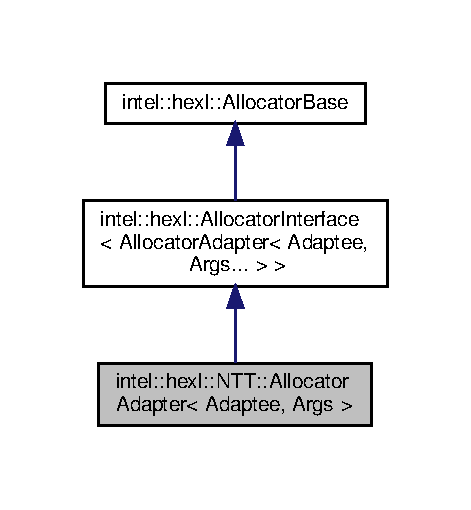
\includegraphics[width=244pt]{structintel_1_1hexl_1_1NTT_1_1AllocatorAdapter__inherit__graph}
\end{center}
\end{figure}


Collaboration diagram for intel\+::hexl\+::N\+TT\+::Allocator\+Adapter$<$ Adaptee, Args $>$\+:
\nopagebreak
\begin{figure}[H]
\begin{center}
\leavevmode
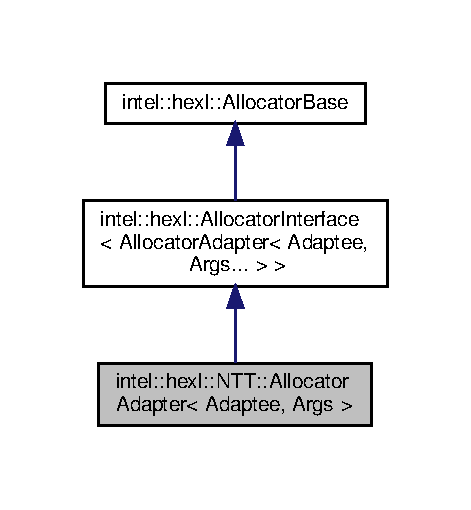
\includegraphics[width=244pt]{structintel_1_1hexl_1_1NTT_1_1AllocatorAdapter__coll__graph}
\end{center}
\end{figure}
\doxysubsection*{Public Member Functions}
\begin{DoxyCompactItemize}
\item 
\mbox{\hyperlink{structintel_1_1hexl_1_1NTT_1_1AllocatorAdapter_a4403f32f5ed5527a13c2bf12c20a68af}{Allocator\+Adapter}} (Adaptee \&\&\+\_\+a, Args \&\&... args)
\item 
\mbox{\hyperlink{structintel_1_1hexl_1_1NTT_1_1AllocatorAdapter_aee97fbd36cf2299db87f6dbe75f12396}{Allocator\+Adapter}} (const Adaptee \&\+\_\+a, Args \&... args)
\item 
void $\ast$ \mbox{\hyperlink{structintel_1_1hexl_1_1NTT_1_1AllocatorAdapter_a408a6a4b42aef1db5ab7e9b5c8ec2670}{allocate\+\_\+impl}} (size\+\_\+t bytes\+\_\+count)
\item 
void \mbox{\hyperlink{structintel_1_1hexl_1_1NTT_1_1AllocatorAdapter_a123aa02665ce9f2b219ca9b88164e114}{deallocate\+\_\+impl}} (void $\ast$p, size\+\_\+t n)
\end{DoxyCompactItemize}


\doxysubsection{Detailed Description}
\subsubsection*{template$<$class Adaptee, class... Args$>$\newline
struct intel\+::hexl\+::\+N\+T\+T\+::\+Allocator\+Adapter$<$ Adaptee, Args $>$}

Helper class for custom memory allocation. 

\doxysubsection{Constructor \& Destructor Documentation}
\mbox{\Hypertarget{structintel_1_1hexl_1_1NTT_1_1AllocatorAdapter_a4403f32f5ed5527a13c2bf12c20a68af}\label{structintel_1_1hexl_1_1NTT_1_1AllocatorAdapter_a4403f32f5ed5527a13c2bf12c20a68af}} 
\index{intel::hexl::NTT::AllocatorAdapter$<$ Adaptee, Args $>$@{intel::hexl::NTT::AllocatorAdapter$<$ Adaptee, Args $>$}!AllocatorAdapter@{AllocatorAdapter}}
\index{AllocatorAdapter@{AllocatorAdapter}!intel::hexl::NTT::AllocatorAdapter$<$ Adaptee, Args $>$@{intel::hexl::NTT::AllocatorAdapter$<$ Adaptee, Args $>$}}
\doxysubsubsection{\texorpdfstring{AllocatorAdapter()}{AllocatorAdapter()}\hspace{0.1cm}{\footnotesize\ttfamily [1/2]}}
{\footnotesize\ttfamily template$<$class Adaptee , class... Args$>$ \\
\mbox{\hyperlink{structintel_1_1hexl_1_1NTT_1_1AllocatorAdapter}{intel\+::hexl\+::\+N\+T\+T\+::\+Allocator\+Adapter}}$<$ Adaptee, Args $>$\+::\mbox{\hyperlink{structintel_1_1hexl_1_1NTT_1_1AllocatorAdapter}{Allocator\+Adapter}} (\begin{DoxyParamCaption}\item[{Adaptee \&\&}]{\+\_\+a,  }\item[{Args \&\&...}]{args }\end{DoxyParamCaption})\hspace{0.3cm}{\ttfamily [explicit]}}

\mbox{\Hypertarget{structintel_1_1hexl_1_1NTT_1_1AllocatorAdapter_aee97fbd36cf2299db87f6dbe75f12396}\label{structintel_1_1hexl_1_1NTT_1_1AllocatorAdapter_aee97fbd36cf2299db87f6dbe75f12396}} 
\index{intel::hexl::NTT::AllocatorAdapter$<$ Adaptee, Args $>$@{intel::hexl::NTT::AllocatorAdapter$<$ Adaptee, Args $>$}!AllocatorAdapter@{AllocatorAdapter}}
\index{AllocatorAdapter@{AllocatorAdapter}!intel::hexl::NTT::AllocatorAdapter$<$ Adaptee, Args $>$@{intel::hexl::NTT::AllocatorAdapter$<$ Adaptee, Args $>$}}
\doxysubsubsection{\texorpdfstring{AllocatorAdapter()}{AllocatorAdapter()}\hspace{0.1cm}{\footnotesize\ttfamily [2/2]}}
{\footnotesize\ttfamily template$<$class Adaptee , class... Args$>$ \\
\mbox{\hyperlink{structintel_1_1hexl_1_1NTT_1_1AllocatorAdapter}{intel\+::hexl\+::\+N\+T\+T\+::\+Allocator\+Adapter}}$<$ Adaptee, Args $>$\+::\mbox{\hyperlink{structintel_1_1hexl_1_1NTT_1_1AllocatorAdapter}{Allocator\+Adapter}} (\begin{DoxyParamCaption}\item[{const Adaptee \&}]{\+\_\+a,  }\item[{Args \&...}]{args }\end{DoxyParamCaption})}



\doxysubsection{Member Function Documentation}
\mbox{\Hypertarget{structintel_1_1hexl_1_1NTT_1_1AllocatorAdapter_a408a6a4b42aef1db5ab7e9b5c8ec2670}\label{structintel_1_1hexl_1_1NTT_1_1AllocatorAdapter_a408a6a4b42aef1db5ab7e9b5c8ec2670}} 
\index{intel::hexl::NTT::AllocatorAdapter$<$ Adaptee, Args $>$@{intel::hexl::NTT::AllocatorAdapter$<$ Adaptee, Args $>$}!allocate\_impl@{allocate\_impl}}
\index{allocate\_impl@{allocate\_impl}!intel::hexl::NTT::AllocatorAdapter$<$ Adaptee, Args $>$@{intel::hexl::NTT::AllocatorAdapter$<$ Adaptee, Args $>$}}
\doxysubsubsection{\texorpdfstring{allocate\_impl()}{allocate\_impl()}}
{\footnotesize\ttfamily template$<$class Adaptee , class... Args$>$ \\
void$\ast$ \mbox{\hyperlink{structintel_1_1hexl_1_1NTT_1_1AllocatorAdapter}{intel\+::hexl\+::\+N\+T\+T\+::\+Allocator\+Adapter}}$<$ Adaptee, Args $>$\+::allocate\+\_\+impl (\begin{DoxyParamCaption}\item[{size\+\_\+t}]{bytes\+\_\+count }\end{DoxyParamCaption})}

\mbox{\Hypertarget{structintel_1_1hexl_1_1NTT_1_1AllocatorAdapter_a123aa02665ce9f2b219ca9b88164e114}\label{structintel_1_1hexl_1_1NTT_1_1AllocatorAdapter_a123aa02665ce9f2b219ca9b88164e114}} 
\index{intel::hexl::NTT::AllocatorAdapter$<$ Adaptee, Args $>$@{intel::hexl::NTT::AllocatorAdapter$<$ Adaptee, Args $>$}!deallocate\_impl@{deallocate\_impl}}
\index{deallocate\_impl@{deallocate\_impl}!intel::hexl::NTT::AllocatorAdapter$<$ Adaptee, Args $>$@{intel::hexl::NTT::AllocatorAdapter$<$ Adaptee, Args $>$}}
\doxysubsubsection{\texorpdfstring{deallocate\_impl()}{deallocate\_impl()}}
{\footnotesize\ttfamily template$<$class Adaptee , class... Args$>$ \\
void \mbox{\hyperlink{structintel_1_1hexl_1_1NTT_1_1AllocatorAdapter}{intel\+::hexl\+::\+N\+T\+T\+::\+Allocator\+Adapter}}$<$ Adaptee, Args $>$\+::deallocate\+\_\+impl (\begin{DoxyParamCaption}\item[{void $\ast$}]{p,  }\item[{size\+\_\+t}]{n }\end{DoxyParamCaption})}



The documentation for this struct was generated from the following file\+:\begin{DoxyCompactItemize}
\item 
\mbox{\hyperlink{ntt_8hpp}{ntt.\+hpp}}\end{DoxyCompactItemize}

\hypertarget{structintel_1_1hexl_1_1AllocatorBase}{}\section{intel\+:\+:hexl\+:\+:Allocator\+Base Struct Reference}
\label{structintel_1_1hexl_1_1AllocatorBase}\index{intel\+::hexl\+::\+Allocator\+Base@{intel\+::hexl\+::\+Allocator\+Base}}


Base class for custom memory allocator.  




{\ttfamily \#include $<$allocator.\+hpp$>$}



Inheritance diagram for intel\+:\+:hexl\+:\+:Allocator\+Base\+:
\nopagebreak
\begin{figure}[H]
\begin{center}
\leavevmode
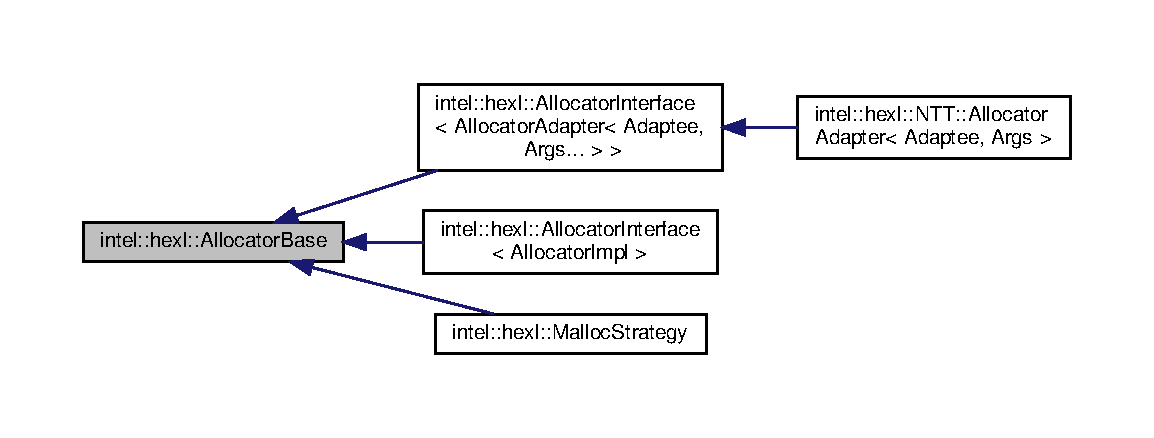
\includegraphics[width=350pt]{structintel_1_1hexl_1_1AllocatorBase__inherit__graph}
\end{center}
\end{figure}
\subsection*{Public Member Functions}
\begin{DoxyCompactItemize}
\item 
virtual \hyperlink{structintel_1_1hexl_1_1AllocatorBase_ac8a2afdc70cef8b7c9342aa2281ea4d5}{$\sim$\+Allocator\+Base} () noexcept
\item 
virtual void $\ast$ \hyperlink{structintel_1_1hexl_1_1AllocatorBase_aadf587e7617fbace2e9d3b4f9d9e8af0}{allocate} (size\+\_\+t bytes\+\_\+count)=0
\begin{DoxyCompactList}\small\item\em Allocates byte\+\_\+count bytes of memory. \end{DoxyCompactList}\item 
virtual void \hyperlink{structintel_1_1hexl_1_1AllocatorBase_a0f03686f9b78728d4d228ceaf4c2948e}{deallocate} (void $\ast$p, size\+\_\+t n)=0
\begin{DoxyCompactList}\small\item\em Deallocate memory. \end{DoxyCompactList}\end{DoxyCompactItemize}


\subsection{Detailed Description}
Base class for custom memory allocator. 

\subsection{Constructor \& Destructor Documentation}
\mbox{\Hypertarget{structintel_1_1hexl_1_1AllocatorBase_ac8a2afdc70cef8b7c9342aa2281ea4d5}\label{structintel_1_1hexl_1_1AllocatorBase_ac8a2afdc70cef8b7c9342aa2281ea4d5}} 
\index{intel\+::hexl\+::\+Allocator\+Base@{intel\+::hexl\+::\+Allocator\+Base}!````~Allocator\+Base@{$\sim$\+Allocator\+Base}}
\index{````~Allocator\+Base@{$\sim$\+Allocator\+Base}!intel\+::hexl\+::\+Allocator\+Base@{intel\+::hexl\+::\+Allocator\+Base}}
\subsubsection{\texorpdfstring{$\sim$\+Allocator\+Base()}{~AllocatorBase()}}
{\footnotesize\ttfamily virtual intel\+::hexl\+::\+Allocator\+Base\+::$\sim$\+Allocator\+Base (\begin{DoxyParamCaption}{ }\end{DoxyParamCaption})\hspace{0.3cm}{\ttfamily [inline]}, {\ttfamily [virtual]}, {\ttfamily [noexcept]}}



\subsection{Member Function Documentation}
\mbox{\Hypertarget{structintel_1_1hexl_1_1AllocatorBase_aadf587e7617fbace2e9d3b4f9d9e8af0}\label{structintel_1_1hexl_1_1AllocatorBase_aadf587e7617fbace2e9d3b4f9d9e8af0}} 
\index{intel\+::hexl\+::\+Allocator\+Base@{intel\+::hexl\+::\+Allocator\+Base}!allocate@{allocate}}
\index{allocate@{allocate}!intel\+::hexl\+::\+Allocator\+Base@{intel\+::hexl\+::\+Allocator\+Base}}
\subsubsection{\texorpdfstring{allocate()}{allocate()}}
{\footnotesize\ttfamily virtual void$\ast$ intel\+::hexl\+::\+Allocator\+Base\+::allocate (\begin{DoxyParamCaption}\item[{size\+\_\+t}]{bytes\+\_\+count }\end{DoxyParamCaption})\hspace{0.3cm}{\ttfamily [pure virtual]}}



Allocates byte\+\_\+count bytes of memory. 


\begin{DoxyParams}[1]{Parameters}
\mbox{\tt in}  & {\em bytes\+\_\+count} & Number of bytes to allocate \\
\hline
\end{DoxyParams}
\begin{DoxyReturn}{Returns}
A pointer to the allocated memory 
\end{DoxyReturn}


Implemented in \hyperlink{structintel_1_1hexl_1_1AllocatorInterface_a02d2d7918ea916fce443ba2f5dbaa8d1}{intel\+::hexl\+::\+Allocator\+Interface$<$ Allocator\+Impl $>$}, \hyperlink{structintel_1_1hexl_1_1AllocatorInterface_a02d2d7918ea916fce443ba2f5dbaa8d1}{intel\+::hexl\+::\+Allocator\+Interface$<$ Allocator\+Adapter$<$ Adaptee, Args... $>$ $>$}, and \hyperlink{structintel_1_1hexl_1_1MallocStrategy_a010052a3f5e39991d57a38742d853738}{intel\+::hexl\+::\+Malloc\+Strategy}.

\mbox{\Hypertarget{structintel_1_1hexl_1_1AllocatorBase_a0f03686f9b78728d4d228ceaf4c2948e}\label{structintel_1_1hexl_1_1AllocatorBase_a0f03686f9b78728d4d228ceaf4c2948e}} 
\index{intel\+::hexl\+::\+Allocator\+Base@{intel\+::hexl\+::\+Allocator\+Base}!deallocate@{deallocate}}
\index{deallocate@{deallocate}!intel\+::hexl\+::\+Allocator\+Base@{intel\+::hexl\+::\+Allocator\+Base}}
\subsubsection{\texorpdfstring{deallocate()}{deallocate()}}
{\footnotesize\ttfamily virtual void intel\+::hexl\+::\+Allocator\+Base\+::deallocate (\begin{DoxyParamCaption}\item[{void $\ast$}]{p,  }\item[{size\+\_\+t}]{n }\end{DoxyParamCaption})\hspace{0.3cm}{\ttfamily [pure virtual]}}



Deallocate memory. 


\begin{DoxyParams}[1]{Parameters}
\mbox{\tt in}  & {\em p} & Pointer to memory to deallocate \\
\hline
\mbox{\tt in}  & {\em n} & Number of bytes to deallocate \\
\hline
\end{DoxyParams}


Implemented in \hyperlink{structintel_1_1hexl_1_1AllocatorInterface_a2684feec3b8f3cfba626b46912b4cec5}{intel\+::hexl\+::\+Allocator\+Interface$<$ Allocator\+Impl $>$}, \hyperlink{structintel_1_1hexl_1_1AllocatorInterface_a2684feec3b8f3cfba626b46912b4cec5}{intel\+::hexl\+::\+Allocator\+Interface$<$ Allocator\+Adapter$<$ Adaptee, Args... $>$ $>$}, and \hyperlink{structintel_1_1hexl_1_1MallocStrategy_af45ff5d0c9b1e867fac481f447a4569c}{intel\+::hexl\+::\+Malloc\+Strategy}.



The documentation for this struct was generated from the following file\+:\begin{DoxyCompactItemize}
\item 
\hyperlink{allocator_8hpp}{allocator.\+hpp}\end{DoxyCompactItemize}

\hypertarget{structintel_1_1hexl_1_1AllocatorInterface}{}\section{intel\+:\+:hexl\+:\+:Allocator\+Interface$<$ Allocator\+Impl $>$ Struct Template Reference}
\label{structintel_1_1hexl_1_1AllocatorInterface}\index{intel\+::hexl\+::\+Allocator\+Interface$<$ Allocator\+Impl $>$@{intel\+::hexl\+::\+Allocator\+Interface$<$ Allocator\+Impl $>$}}


Helper memory allocation struct which delegates implementation to Allocator\+Impl.  




{\ttfamily \#include $<$allocator.\+hpp$>$}



Inheritance diagram for intel\+:\+:hexl\+:\+:Allocator\+Interface$<$ Allocator\+Impl $>$\+:
\nopagebreak
\begin{figure}[H]
\begin{center}
\leavevmode
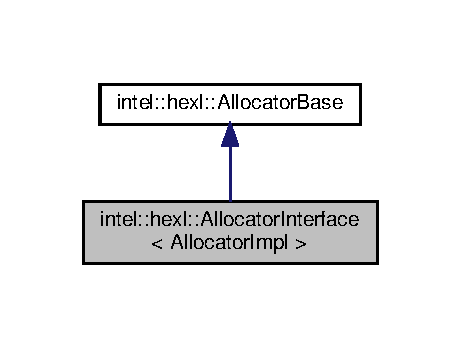
\includegraphics[width=221pt]{structintel_1_1hexl_1_1AllocatorInterface__inherit__graph}
\end{center}
\end{figure}


Collaboration diagram for intel\+:\+:hexl\+:\+:Allocator\+Interface$<$ Allocator\+Impl $>$\+:
\nopagebreak
\begin{figure}[H]
\begin{center}
\leavevmode
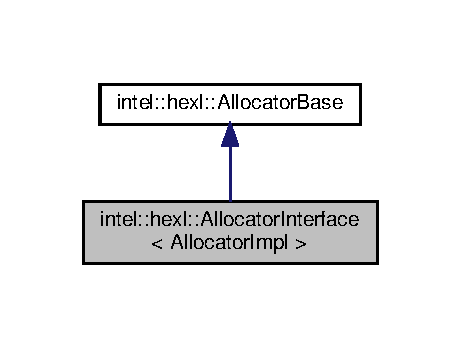
\includegraphics[width=221pt]{structintel_1_1hexl_1_1AllocatorInterface__coll__graph}
\end{center}
\end{figure}
\subsection*{Public Member Functions}
\begin{DoxyCompactItemize}
\item 
void $\ast$ \hyperlink{structintel_1_1hexl_1_1AllocatorInterface_a02d2d7918ea916fce443ba2f5dbaa8d1}{allocate} (size\+\_\+t bytes\+\_\+count) override
\begin{DoxyCompactList}\small\item\em Override interface and delegate implementation to Allocator\+Impl. \end{DoxyCompactList}\item 
void \hyperlink{structintel_1_1hexl_1_1AllocatorInterface_a2684feec3b8f3cfba626b46912b4cec5}{deallocate} (void $\ast$p, size\+\_\+t n) override
\begin{DoxyCompactList}\small\item\em Override interface and delegate implementation to Allocator\+Impl. \end{DoxyCompactList}\end{DoxyCompactItemize}


\subsection{Detailed Description}
\subsubsection*{template$<$class Allocator\+Impl$>$\newline
struct intel\+::hexl\+::\+Allocator\+Interface$<$ Allocator\+Impl $>$}

Helper memory allocation struct which delegates implementation to Allocator\+Impl. 

\subsection{Member Function Documentation}
\mbox{\Hypertarget{structintel_1_1hexl_1_1AllocatorInterface_a02d2d7918ea916fce443ba2f5dbaa8d1}\label{structintel_1_1hexl_1_1AllocatorInterface_a02d2d7918ea916fce443ba2f5dbaa8d1}} 
\index{intel\+::hexl\+::\+Allocator\+Interface@{intel\+::hexl\+::\+Allocator\+Interface}!allocate@{allocate}}
\index{allocate@{allocate}!intel\+::hexl\+::\+Allocator\+Interface@{intel\+::hexl\+::\+Allocator\+Interface}}
\subsubsection{\texorpdfstring{allocate()}{allocate()}}
{\footnotesize\ttfamily template$<$class Allocator\+Impl$>$ \\
void$\ast$ \hyperlink{structintel_1_1hexl_1_1AllocatorInterface}{intel\+::hexl\+::\+Allocator\+Interface}$<$ Allocator\+Impl $>$\+::allocate (\begin{DoxyParamCaption}\item[{size\+\_\+t}]{bytes\+\_\+count }\end{DoxyParamCaption})\hspace{0.3cm}{\ttfamily [inline]}, {\ttfamily [override]}, {\ttfamily [virtual]}}



Override interface and delegate implementation to Allocator\+Impl. 



Implements \hyperlink{structintel_1_1hexl_1_1AllocatorBase_aadf587e7617fbace2e9d3b4f9d9e8af0}{intel\+::hexl\+::\+Allocator\+Base}.

\mbox{\Hypertarget{structintel_1_1hexl_1_1AllocatorInterface_a2684feec3b8f3cfba626b46912b4cec5}\label{structintel_1_1hexl_1_1AllocatorInterface_a2684feec3b8f3cfba626b46912b4cec5}} 
\index{intel\+::hexl\+::\+Allocator\+Interface@{intel\+::hexl\+::\+Allocator\+Interface}!deallocate@{deallocate}}
\index{deallocate@{deallocate}!intel\+::hexl\+::\+Allocator\+Interface@{intel\+::hexl\+::\+Allocator\+Interface}}
\subsubsection{\texorpdfstring{deallocate()}{deallocate()}}
{\footnotesize\ttfamily template$<$class Allocator\+Impl$>$ \\
void \hyperlink{structintel_1_1hexl_1_1AllocatorInterface}{intel\+::hexl\+::\+Allocator\+Interface}$<$ Allocator\+Impl $>$\+::deallocate (\begin{DoxyParamCaption}\item[{void $\ast$}]{p,  }\item[{size\+\_\+t}]{n }\end{DoxyParamCaption})\hspace{0.3cm}{\ttfamily [inline]}, {\ttfamily [override]}, {\ttfamily [virtual]}}



Override interface and delegate implementation to Allocator\+Impl. 



Implements \hyperlink{structintel_1_1hexl_1_1AllocatorBase_a0f03686f9b78728d4d228ceaf4c2948e}{intel\+::hexl\+::\+Allocator\+Base}.



The documentation for this struct was generated from the following file\+:\begin{DoxyCompactItemize}
\item 
\hyperlink{allocator_8hpp}{allocator.\+hpp}\end{DoxyCompactItemize}

\hypertarget{structintel_1_1hexl_1_1MallocStrategy}{}\doxysection{intel\+::hexl\+::Malloc\+Strategy Struct Reference}
\label{structintel_1_1hexl_1_1MallocStrategy}\index{intel::hexl::MallocStrategy@{intel::hexl::MallocStrategy}}


Allocater implementation using malloc and free.  




{\ttfamily \#include $<$aligned-\/allocator.\+hpp$>$}



Inheritance diagram for intel\+::hexl\+::Malloc\+Strategy\+:
\nopagebreak
\begin{figure}[H]
\begin{center}
\leavevmode
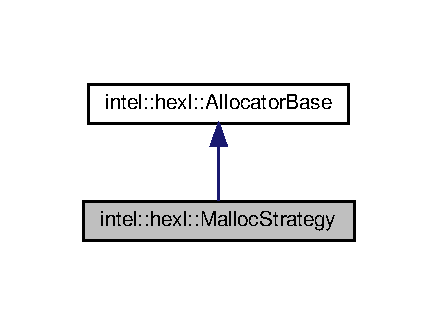
\includegraphics[width=225pt]{structintel_1_1hexl_1_1MallocStrategy__inherit__graph}
\end{center}
\end{figure}


Collaboration diagram for intel\+::hexl\+::Malloc\+Strategy\+:
\nopagebreak
\begin{figure}[H]
\begin{center}
\leavevmode
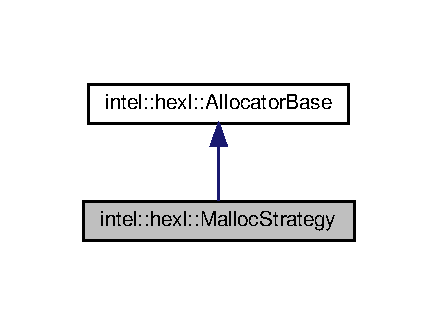
\includegraphics[width=225pt]{structintel_1_1hexl_1_1MallocStrategy__coll__graph}
\end{center}
\end{figure}
\doxysubsection*{Public Member Functions}
\begin{DoxyCompactItemize}
\item 
void $\ast$ \mbox{\hyperlink{structintel_1_1hexl_1_1MallocStrategy_a010052a3f5e39991d57a38742d853738}{allocate}} (size\+\_\+t bytes\+\_\+count) final
\begin{DoxyCompactList}\small\item\em Allocates byte\+\_\+count bytes of memory. \end{DoxyCompactList}\item 
void \mbox{\hyperlink{structintel_1_1hexl_1_1MallocStrategy_af45ff5d0c9b1e867fac481f447a4569c}{deallocate}} (void $\ast$p, size\+\_\+t n) final
\begin{DoxyCompactList}\small\item\em Deallocate memory. \end{DoxyCompactList}\end{DoxyCompactItemize}


\doxysubsection{Detailed Description}
Allocater implementation using malloc and free. 

\doxysubsection{Member Function Documentation}
\mbox{\Hypertarget{structintel_1_1hexl_1_1MallocStrategy_a010052a3f5e39991d57a38742d853738}\label{structintel_1_1hexl_1_1MallocStrategy_a010052a3f5e39991d57a38742d853738}} 
\index{intel::hexl::MallocStrategy@{intel::hexl::MallocStrategy}!allocate@{allocate}}
\index{allocate@{allocate}!intel::hexl::MallocStrategy@{intel::hexl::MallocStrategy}}
\doxysubsubsection{\texorpdfstring{allocate()}{allocate()}}
{\footnotesize\ttfamily void$\ast$ intel\+::hexl\+::\+Malloc\+Strategy\+::allocate (\begin{DoxyParamCaption}\item[{size\+\_\+t}]{bytes\+\_\+count }\end{DoxyParamCaption})\hspace{0.3cm}{\ttfamily [inline]}, {\ttfamily [final]}, {\ttfamily [virtual]}}



Allocates byte\+\_\+count bytes of memory. 


\begin{DoxyParams}[1]{Parameters}
\mbox{\texttt{ in}}  & {\em bytes\+\_\+count} & Number of bytes to allocate \\
\hline
\end{DoxyParams}
\begin{DoxyReturn}{Returns}
A pointer to the allocated memory 
\end{DoxyReturn}


Implements \mbox{\hyperlink{structintel_1_1hexl_1_1AllocatorBase_aadf587e7617fbace2e9d3b4f9d9e8af0}{intel\+::hexl\+::\+Allocator\+Base}}.

\mbox{\Hypertarget{structintel_1_1hexl_1_1MallocStrategy_af45ff5d0c9b1e867fac481f447a4569c}\label{structintel_1_1hexl_1_1MallocStrategy_af45ff5d0c9b1e867fac481f447a4569c}} 
\index{intel::hexl::MallocStrategy@{intel::hexl::MallocStrategy}!deallocate@{deallocate}}
\index{deallocate@{deallocate}!intel::hexl::MallocStrategy@{intel::hexl::MallocStrategy}}
\doxysubsubsection{\texorpdfstring{deallocate()}{deallocate()}}
{\footnotesize\ttfamily void intel\+::hexl\+::\+Malloc\+Strategy\+::deallocate (\begin{DoxyParamCaption}\item[{void $\ast$}]{p,  }\item[{size\+\_\+t}]{n }\end{DoxyParamCaption})\hspace{0.3cm}{\ttfamily [inline]}, {\ttfamily [final]}, {\ttfamily [virtual]}}



Deallocate memory. 


\begin{DoxyParams}[1]{Parameters}
\mbox{\texttt{ in}}  & {\em p} & Pointer to memory to deallocate \\
\hline
\mbox{\texttt{ in}}  & {\em n} & Number of bytes to deallocate \\
\hline
\end{DoxyParams}


Implements \mbox{\hyperlink{structintel_1_1hexl_1_1AllocatorBase_a0f03686f9b78728d4d228ceaf4c2948e}{intel\+::hexl\+::\+Allocator\+Base}}.



The documentation for this struct was generated from the following file\+:\begin{DoxyCompactItemize}
\item 
\mbox{\hyperlink{aligned-allocator_8hpp}{aligned-\/allocator.\+hpp}}\end{DoxyCompactItemize}

\hypertarget{classintel_1_1hexl_1_1MultiplyFactor}{}\doxysection{intel\+::hexl\+::Multiply\+Factor Class Reference}
\label{classintel_1_1hexl_1_1MultiplyFactor}\index{intel::hexl::MultiplyFactor@{intel::hexl::MultiplyFactor}}


Pre-\/computes a Barrett factor with which modular multiplication can be performed more efficiently.  




{\ttfamily \#include $<$number-\/theory.\+hpp$>$}

\doxysubsection*{Public Member Functions}
\begin{DoxyCompactItemize}
\item 
\mbox{\hyperlink{classintel_1_1hexl_1_1MultiplyFactor_ad7b998b4a54203d6ad83237e3b3f4c51}{Multiply\+Factor}} ()=default
\item 
\mbox{\hyperlink{classintel_1_1hexl_1_1MultiplyFactor_a801de0aa37e108b21cdb6452a15f6c76}{Multiply\+Factor}} (uint64\+\_\+t operand, uint64\+\_\+t bit\+\_\+shift, uint64\+\_\+t modulus)
\begin{DoxyCompactList}\small\item\em Computes and stores the Barrett factor floor((operand $<$$<$ bit\+\_\+shift) / modulus). This is useful when modular multiplication of the form (x $\ast$ operand) mod modulus is performed with same modulus and operand several times. Note, passing operand=1 can be used to pre-\/compute a Barrett factor for multiplications of the form (x $\ast$ y) mod modulus, where only the modulus is re-\/used across calls to modular multiplication. \end{DoxyCompactList}\item 
uint64\+\_\+t \mbox{\hyperlink{classintel_1_1hexl_1_1MultiplyFactor_aa1708edda697a2ebb93f6b2b9b2967aa}{Barrett\+Factor}} () const
\begin{DoxyCompactList}\small\item\em Returns the pre-\/computed Barrett factor. \end{DoxyCompactList}\item 
uint64\+\_\+t \mbox{\hyperlink{classintel_1_1hexl_1_1MultiplyFactor_a143d0ed636511f3cd450286b89687822}{Operand}} () const
\begin{DoxyCompactList}\small\item\em Returns the operand corresponding to the Barrett factor. \end{DoxyCompactList}\end{DoxyCompactItemize}


\doxysubsection{Detailed Description}
Pre-\/computes a Barrett factor with which modular multiplication can be performed more efficiently. 

\doxysubsection{Constructor \& Destructor Documentation}
\mbox{\Hypertarget{classintel_1_1hexl_1_1MultiplyFactor_ad7b998b4a54203d6ad83237e3b3f4c51}\label{classintel_1_1hexl_1_1MultiplyFactor_ad7b998b4a54203d6ad83237e3b3f4c51}} 
\index{intel::hexl::MultiplyFactor@{intel::hexl::MultiplyFactor}!MultiplyFactor@{MultiplyFactor}}
\index{MultiplyFactor@{MultiplyFactor}!intel::hexl::MultiplyFactor@{intel::hexl::MultiplyFactor}}
\doxysubsubsection{\texorpdfstring{MultiplyFactor()}{MultiplyFactor()}\hspace{0.1cm}{\footnotesize\ttfamily [1/2]}}
{\footnotesize\ttfamily intel\+::hexl\+::\+Multiply\+Factor\+::\+Multiply\+Factor (\begin{DoxyParamCaption}{ }\end{DoxyParamCaption})\hspace{0.3cm}{\ttfamily [default]}}

\mbox{\Hypertarget{classintel_1_1hexl_1_1MultiplyFactor_a801de0aa37e108b21cdb6452a15f6c76}\label{classintel_1_1hexl_1_1MultiplyFactor_a801de0aa37e108b21cdb6452a15f6c76}} 
\index{intel::hexl::MultiplyFactor@{intel::hexl::MultiplyFactor}!MultiplyFactor@{MultiplyFactor}}
\index{MultiplyFactor@{MultiplyFactor}!intel::hexl::MultiplyFactor@{intel::hexl::MultiplyFactor}}
\doxysubsubsection{\texorpdfstring{MultiplyFactor()}{MultiplyFactor()}\hspace{0.1cm}{\footnotesize\ttfamily [2/2]}}
{\footnotesize\ttfamily intel\+::hexl\+::\+Multiply\+Factor\+::\+Multiply\+Factor (\begin{DoxyParamCaption}\item[{uint64\+\_\+t}]{operand,  }\item[{uint64\+\_\+t}]{bit\+\_\+shift,  }\item[{uint64\+\_\+t}]{modulus }\end{DoxyParamCaption})\hspace{0.3cm}{\ttfamily [inline]}}



Computes and stores the Barrett factor floor((operand $<$$<$ bit\+\_\+shift) / modulus). This is useful when modular multiplication of the form (x $\ast$ operand) mod modulus is performed with same modulus and operand several times. Note, passing operand=1 can be used to pre-\/compute a Barrett factor for multiplications of the form (x $\ast$ y) mod modulus, where only the modulus is re-\/used across calls to modular multiplication. 



\doxysubsection{Member Function Documentation}
\mbox{\Hypertarget{classintel_1_1hexl_1_1MultiplyFactor_aa1708edda697a2ebb93f6b2b9b2967aa}\label{classintel_1_1hexl_1_1MultiplyFactor_aa1708edda697a2ebb93f6b2b9b2967aa}} 
\index{intel::hexl::MultiplyFactor@{intel::hexl::MultiplyFactor}!BarrettFactor@{BarrettFactor}}
\index{BarrettFactor@{BarrettFactor}!intel::hexl::MultiplyFactor@{intel::hexl::MultiplyFactor}}
\doxysubsubsection{\texorpdfstring{BarrettFactor()}{BarrettFactor()}}
{\footnotesize\ttfamily uint64\+\_\+t intel\+::hexl\+::\+Multiply\+Factor\+::\+Barrett\+Factor (\begin{DoxyParamCaption}{ }\end{DoxyParamCaption}) const\hspace{0.3cm}{\ttfamily [inline]}}



Returns the pre-\/computed Barrett factor. 

\mbox{\Hypertarget{classintel_1_1hexl_1_1MultiplyFactor_a143d0ed636511f3cd450286b89687822}\label{classintel_1_1hexl_1_1MultiplyFactor_a143d0ed636511f3cd450286b89687822}} 
\index{intel::hexl::MultiplyFactor@{intel::hexl::MultiplyFactor}!Operand@{Operand}}
\index{Operand@{Operand}!intel::hexl::MultiplyFactor@{intel::hexl::MultiplyFactor}}
\doxysubsubsection{\texorpdfstring{Operand()}{Operand()}}
{\footnotesize\ttfamily uint64\+\_\+t intel\+::hexl\+::\+Multiply\+Factor\+::\+Operand (\begin{DoxyParamCaption}{ }\end{DoxyParamCaption}) const\hspace{0.3cm}{\ttfamily [inline]}}



Returns the operand corresponding to the Barrett factor. 



The documentation for this class was generated from the following file\+:\begin{DoxyCompactItemize}
\item 
\mbox{\hyperlink{number-theory_8hpp}{number-\/theory.\+hpp}}\end{DoxyCompactItemize}

\hypertarget{classintel_1_1hexl_1_1NTT}{}\doxysection{intel\+::hexl\+::N\+TT Class Reference}
\label{classintel_1_1hexl_1_1NTT}\index{intel::hexl::NTT@{intel::hexl::NTT}}


Performs negacyclic forward and inverse number-\/theoretic transform (\mbox{\hyperlink{classintel_1_1hexl_1_1NTT}{N\+TT}}), commonly used in R\+L\+WE cryptography.  




{\ttfamily \#include $<$ntt.\+hpp$>$}

\doxysubsection*{Classes}
\begin{DoxyCompactItemize}
\item 
struct \mbox{\hyperlink{structintel_1_1hexl_1_1NTT_1_1AllocatorAdapter}{Allocator\+Adapter}}
\begin{DoxyCompactList}\small\item\em Helper class for custom memory allocation. \end{DoxyCompactList}\end{DoxyCompactItemize}
\doxysubsection*{Public Member Functions}
\begin{DoxyCompactItemize}
\item 
\mbox{\hyperlink{classintel_1_1hexl_1_1NTT_ad31a184065b07b50c3ff01260f6dad28}{N\+TT}} ()=default
\begin{DoxyCompactList}\small\item\em Initializes an empty \mbox{\hyperlink{classintel_1_1hexl_1_1NTT}{N\+TT}} object. \end{DoxyCompactList}\item 
\mbox{\hyperlink{classintel_1_1hexl_1_1NTT_a4fbb886db7389f6a5bac264a3e0cf66f}{$\sim$\+N\+TT}} ()=default
\begin{DoxyCompactList}\small\item\em Destructs the \mbox{\hyperlink{classintel_1_1hexl_1_1NTT}{N\+TT}} object. \end{DoxyCompactList}\item 
\mbox{\hyperlink{classintel_1_1hexl_1_1NTT_a7a86355beefbe191d0e77618eeaaf6b7}{N\+TT}} (uint64\+\_\+t degree, uint64\+\_\+t q, std\+::shared\+\_\+ptr$<$ \mbox{\hyperlink{structintel_1_1hexl_1_1AllocatorBase}{Allocator\+Base}} $>$ alloc\+\_\+ptr=\{\})
\begin{DoxyCompactList}\small\item\em Initializes an \mbox{\hyperlink{classintel_1_1hexl_1_1NTT}{N\+TT}} object with degree {\ttfamily degree} and modulus {\ttfamily q}. \end{DoxyCompactList}\item 
{\footnotesize template$<$class Allocator , class... Allocator\+Args$>$ }\\\mbox{\hyperlink{classintel_1_1hexl_1_1NTT_a716fd07255e9b68fec80e2a9b98841f4}{N\+TT}} (uint64\+\_\+t degree, uint64\+\_\+t q, Allocator \&\&a, Allocator\+Args \&\&... args)
\item 
\mbox{\hyperlink{classintel_1_1hexl_1_1NTT_ac5ef577bf39789c1e200b7d5a7b65989}{N\+TT}} (uint64\+\_\+t degree, uint64\+\_\+t q, uint64\+\_\+t root\+\_\+of\+\_\+unity, std\+::shared\+\_\+ptr$<$ \mbox{\hyperlink{structintel_1_1hexl_1_1AllocatorBase}{Allocator\+Base}} $>$ alloc\+\_\+ptr=\{\})
\begin{DoxyCompactList}\small\item\em Initializes an \mbox{\hyperlink{classintel_1_1hexl_1_1NTT}{N\+TT}} object with degree {\ttfamily degree} and modulus {\ttfamily q}. \end{DoxyCompactList}\item 
{\footnotesize template$<$class Allocator , class... Allocator\+Args$>$ }\\\mbox{\hyperlink{classintel_1_1hexl_1_1NTT_a831df901cf9ea5a83e5d628cdbd36671}{N\+TT}} (uint64\+\_\+t degree, uint64\+\_\+t q, uint64\+\_\+t root\+\_\+of\+\_\+unity, Allocator \&\&a, Allocator\+Args \&\&... args)
\item 
void \mbox{\hyperlink{classintel_1_1hexl_1_1NTT_a7f8dac5ff3fc117d3e7259762a716140}{Compute\+Forward}} (uint64\+\_\+t $\ast$result, const uint64\+\_\+t $\ast$operand, uint64\+\_\+t input\+\_\+mod\+\_\+factor, uint64\+\_\+t output\+\_\+mod\+\_\+factor)
\begin{DoxyCompactList}\small\item\em Compute forward \mbox{\hyperlink{classintel_1_1hexl_1_1NTT}{N\+TT}}. Results are bit-\/reversed. \end{DoxyCompactList}\item 
void \mbox{\hyperlink{classintel_1_1hexl_1_1NTT_a31e78375dcafd5df85cb1259a9156a9a}{Compute\+Inverse}} (uint64\+\_\+t $\ast$result, const uint64\+\_\+t $\ast$operand, uint64\+\_\+t input\+\_\+mod\+\_\+factor, uint64\+\_\+t output\+\_\+mod\+\_\+factor)
\item 
uint64\+\_\+t \mbox{\hyperlink{classintel_1_1hexl_1_1NTT_af10476eb10c3b5723052bdf59d7f3d22}{Get\+Minimal\+Root\+Of\+Unity}} () const
\begin{DoxyCompactList}\small\item\em Returns the minimal 2N\textquotesingle{}th root of unity. \end{DoxyCompactList}\item 
uint64\+\_\+t \mbox{\hyperlink{classintel_1_1hexl_1_1NTT_a25172ec87ce3cbfe9bbc20cd9c52f2ab}{Get\+Degree}} () const
\begin{DoxyCompactList}\small\item\em Returns the degree N. \end{DoxyCompactList}\item 
uint64\+\_\+t \mbox{\hyperlink{classintel_1_1hexl_1_1NTT_aef2a5afbd559f7e27d5fa7d4e28bd252}{Get\+Modulus}} () const
\begin{DoxyCompactList}\small\item\em Returns the word-\/sized prime modulus. \end{DoxyCompactList}\item 
const \mbox{\hyperlink{namespaceintel_1_1hexl_afbdf0d2cc4209ee547a88ff22a02801b}{Aligned\+Vector64}}$<$ uint64\+\_\+t $>$ \& \mbox{\hyperlink{classintel_1_1hexl_1_1NTT_a71749beadc3fde1d2b80f2d99b739099}{Get\+Root\+Of\+Unity\+Powers}} () const
\begin{DoxyCompactList}\small\item\em Returns the root of unity powers in bit-\/reversed order. \end{DoxyCompactList}\item 
uint64\+\_\+t \mbox{\hyperlink{classintel_1_1hexl_1_1NTT_af0ab14a87e3f9e8cf46502c4c766fec5}{Get\+Root\+Of\+Unity\+Power}} (size\+\_\+t i)
\begin{DoxyCompactList}\small\item\em Returns the root of unity power at bit-\/reversed index i. \end{DoxyCompactList}\item 
const \mbox{\hyperlink{namespaceintel_1_1hexl_afbdf0d2cc4209ee547a88ff22a02801b}{Aligned\+Vector64}}$<$ uint64\+\_\+t $>$ \& \mbox{\hyperlink{classintel_1_1hexl_1_1NTT_a1cbd65fb426faafbd22fcb8b7ee98807}{Get\+Precon32\+Root\+Of\+Unity\+Powers}} () const
\begin{DoxyCompactList}\small\item\em Returns 32-\/bit pre-\/conditioned root of unity powers in bit-\/reversed order. \end{DoxyCompactList}\item 
const \mbox{\hyperlink{namespaceintel_1_1hexl_afbdf0d2cc4209ee547a88ff22a02801b}{Aligned\+Vector64}}$<$ uint64\+\_\+t $>$ \& \mbox{\hyperlink{classintel_1_1hexl_1_1NTT_a3bddde00a1832f4ac175e71469939e51}{Get\+Precon64\+Root\+Of\+Unity\+Powers}} () const
\begin{DoxyCompactList}\small\item\em Returns 64-\/bit pre-\/conditioned root of unity powers in bit-\/reversed order. \end{DoxyCompactList}\item 
const \mbox{\hyperlink{namespaceintel_1_1hexl_afbdf0d2cc4209ee547a88ff22a02801b}{Aligned\+Vector64}}$<$ uint64\+\_\+t $>$ \& \mbox{\hyperlink{classintel_1_1hexl_1_1NTT_ac93455767a667ef07aa41f747c77b4ae}{Get\+A\+V\+X512\+Root\+Of\+Unity\+Powers}} () const
\begin{DoxyCompactList}\small\item\em Returns the root of unity powers in bit-\/reversed order with modifications for use by A\+V\+X512 implementation. \end{DoxyCompactList}\item 
const \mbox{\hyperlink{namespaceintel_1_1hexl_afbdf0d2cc4209ee547a88ff22a02801b}{Aligned\+Vector64}}$<$ uint64\+\_\+t $>$ \& \mbox{\hyperlink{classintel_1_1hexl_1_1NTT_acf8896d7c5ab8c47fe860f3d5a1be215}{Get\+A\+V\+X512\+Precon32\+Root\+Of\+Unity\+Powers}} () const
\begin{DoxyCompactList}\small\item\em Returns 32-\/bit pre-\/conditioned A\+V\+X512 root of unity powers in bit-\/reversed order. \end{DoxyCompactList}\item 
const \mbox{\hyperlink{namespaceintel_1_1hexl_afbdf0d2cc4209ee547a88ff22a02801b}{Aligned\+Vector64}}$<$ uint64\+\_\+t $>$ \& \mbox{\hyperlink{classintel_1_1hexl_1_1NTT_aca9903ac08ed7e06d343f85a0ced8b04}{Get\+A\+V\+X512\+Precon52\+Root\+Of\+Unity\+Powers}} () const
\begin{DoxyCompactList}\small\item\em Returns 52-\/bit pre-\/conditioned A\+V\+X512 root of unity powers in bit-\/reversed order. \end{DoxyCompactList}\item 
const \mbox{\hyperlink{namespaceintel_1_1hexl_afbdf0d2cc4209ee547a88ff22a02801b}{Aligned\+Vector64}}$<$ uint64\+\_\+t $>$ \& \mbox{\hyperlink{classintel_1_1hexl_1_1NTT_afb5b2c6cd1135f708c5e8a4e97d6f7da}{Get\+A\+V\+X512\+Precon64\+Root\+Of\+Unity\+Powers}} () const
\begin{DoxyCompactList}\small\item\em Returns 64-\/bit pre-\/conditioned A\+V\+X512 root of unity powers in bit-\/reversed order. \end{DoxyCompactList}\item 
const \mbox{\hyperlink{namespaceintel_1_1hexl_afbdf0d2cc4209ee547a88ff22a02801b}{Aligned\+Vector64}}$<$ uint64\+\_\+t $>$ \& \mbox{\hyperlink{classintel_1_1hexl_1_1NTT_a509f384895cf97ef9cd2edd2902eb82a}{Get\+Inv\+Root\+Of\+Unity\+Powers}} () const
\begin{DoxyCompactList}\small\item\em Returns the inverse root of unity powers in bit-\/reversed order. \end{DoxyCompactList}\item 
uint64\+\_\+t \mbox{\hyperlink{classintel_1_1hexl_1_1NTT_a7dd5b59ed992c5466099999ce1eb15d6}{Get\+Inv\+Root\+Of\+Unity\+Power}} (size\+\_\+t i)
\begin{DoxyCompactList}\small\item\em Returns the inverse root of unity power at bit-\/reversed index i. \end{DoxyCompactList}\item 
const \mbox{\hyperlink{namespaceintel_1_1hexl_afbdf0d2cc4209ee547a88ff22a02801b}{Aligned\+Vector64}}$<$ uint64\+\_\+t $>$ \& \mbox{\hyperlink{classintel_1_1hexl_1_1NTT_a70d5480692fcd13418ae7f4c38345770}{Get\+Precon32\+Inv\+Root\+Of\+Unity\+Powers}} () const
\begin{DoxyCompactList}\small\item\em Returns the vector of 32-\/bit pre-\/conditioned pre-\/computed root of unity. \end{DoxyCompactList}\item 
const \mbox{\hyperlink{namespaceintel_1_1hexl_afbdf0d2cc4209ee547a88ff22a02801b}{Aligned\+Vector64}}$<$ uint64\+\_\+t $>$ \& \mbox{\hyperlink{classintel_1_1hexl_1_1NTT_a9314e0edf36095233efaf72dc6cb9d5e}{Get\+Precon52\+Inv\+Root\+Of\+Unity\+Powers}} () const
\begin{DoxyCompactList}\small\item\em Returns the vector of 52-\/bit pre-\/conditioned pre-\/computed root of unity. \end{DoxyCompactList}\item 
const \mbox{\hyperlink{namespaceintel_1_1hexl_afbdf0d2cc4209ee547a88ff22a02801b}{Aligned\+Vector64}}$<$ uint64\+\_\+t $>$ \& \mbox{\hyperlink{classintel_1_1hexl_1_1NTT_a0f7f195efe5166b0f3a8c9e71f3a405a}{Get\+Precon64\+Inv\+Root\+Of\+Unity\+Powers}} () const
\begin{DoxyCompactList}\small\item\em Returns the vector of 64-\/bit pre-\/conditioned pre-\/computed root of unity. \end{DoxyCompactList}\end{DoxyCompactItemize}
\doxysubsection*{Static Public Member Functions}
\begin{DoxyCompactItemize}
\item 
static bool \mbox{\hyperlink{classintel_1_1hexl_1_1NTT_a81e461e466f57c1c454564879121d8d3}{Check\+Arguments}} (uint64\+\_\+t degree, uint64\+\_\+t modulus)
\begin{DoxyCompactList}\small\item\em Returns true if arguments satisfy constraints for negacyclic \mbox{\hyperlink{classintel_1_1hexl_1_1NTT}{N\+TT}}. \end{DoxyCompactList}\item 
static size\+\_\+t \mbox{\hyperlink{classintel_1_1hexl_1_1NTT_a76d33e88bd12c2c91b7f8285f8525d72}{Max\+Degree\+Bits}} ()
\begin{DoxyCompactList}\small\item\em Maximum power of 2 in degree. \end{DoxyCompactList}\item 
static size\+\_\+t \mbox{\hyperlink{classintel_1_1hexl_1_1NTT_afa71c9bf13109e0d07cacce9e752357c}{Max\+Modulus\+Bits}} ()
\begin{DoxyCompactList}\small\item\em Maximum number of bits in modulus;. \end{DoxyCompactList}\item 
static size\+\_\+t \mbox{\hyperlink{classintel_1_1hexl_1_1NTT_a000f6353bfff8062664e7086d27c8b06}{s\+\_\+max\+\_\+fwd\+\_\+modulus}} (int bit\+\_\+shift)
\item 
static size\+\_\+t \mbox{\hyperlink{classintel_1_1hexl_1_1NTT_abd4a2ad80ba21dd71c4753187cd6ddea}{s\+\_\+max\+\_\+inv\+\_\+modulus}} (int bit\+\_\+shift)
\end{DoxyCompactItemize}
\doxysubsection*{Static Public Attributes}
\begin{DoxyCompactItemize}
\item 
static const size\+\_\+t \mbox{\hyperlink{classintel_1_1hexl_1_1NTT_ab0db0e033026cff37b7acba889500b6d}{s\+\_\+default\+\_\+shift\+\_\+bits}} \{64\}
\begin{DoxyCompactList}\small\item\em Default bit shift used in Barrett precomputation. \end{DoxyCompactList}\item 
static const size\+\_\+t \mbox{\hyperlink{classintel_1_1hexl_1_1NTT_a5642931d7118e5a6304890f18a92c6dc}{s\+\_\+ifma\+\_\+shift\+\_\+bits}} \{52\}
\begin{DoxyCompactList}\small\item\em Bit shift used in Barrett precomputation when A\+V\+X512-\/\+I\+F\+MA acceleration is enabled. \end{DoxyCompactList}\item 
static const size\+\_\+t \mbox{\hyperlink{classintel_1_1hexl_1_1NTT_a4c42c952781ae97d1abf02ab5334143f}{s\+\_\+max\+\_\+fwd\+\_\+32\+\_\+modulus}} \{1U\+LL $<$$<$ (32 -\/ 2)\}
\begin{DoxyCompactList}\small\item\em Maximum modulus to use 32-\/bit A\+V\+X512-\/\+DQ acceleration for the forward transform. \end{DoxyCompactList}\item 
static const size\+\_\+t \mbox{\hyperlink{classintel_1_1hexl_1_1NTT_a33af06994139ae14c69d8958611487bd}{s\+\_\+max\+\_\+inv\+\_\+32\+\_\+modulus}} \{1U\+LL $<$$<$ (32 -\/ 2)\}
\begin{DoxyCompactList}\small\item\em Maximum modulus to use 32-\/bit A\+V\+X512-\/\+DQ acceleration for the inverse transform. \end{DoxyCompactList}\item 
static const size\+\_\+t \mbox{\hyperlink{classintel_1_1hexl_1_1NTT_a248f7a613b187a7f71a67b93e4ca13ad}{s\+\_\+max\+\_\+fwd\+\_\+ifma\+\_\+modulus}} \{1U\+LL $<$$<$ (\mbox{\hyperlink{classintel_1_1hexl_1_1NTT_a5642931d7118e5a6304890f18a92c6dc}{s\+\_\+ifma\+\_\+shift\+\_\+bits}} -\/ 2)\}
\begin{DoxyCompactList}\small\item\em Maximum modulus to use A\+V\+X512-\/\+I\+F\+MA acceleration for the forward transform. \end{DoxyCompactList}\item 
static const size\+\_\+t \mbox{\hyperlink{classintel_1_1hexl_1_1NTT_a741db1877b630638173b6ed5f9a6e6c7}{s\+\_\+max\+\_\+inv\+\_\+ifma\+\_\+modulus}} \{1U\+LL $<$$<$ (\mbox{\hyperlink{classintel_1_1hexl_1_1NTT_a5642931d7118e5a6304890f18a92c6dc}{s\+\_\+ifma\+\_\+shift\+\_\+bits}} -\/ 2)\}
\begin{DoxyCompactList}\small\item\em Maximum modulus to use A\+V\+X512-\/\+I\+F\+MA acceleration for the inverse transform. \end{DoxyCompactList}\item 
static const size\+\_\+t \mbox{\hyperlink{classintel_1_1hexl_1_1NTT_ae5c701d4ff1d90d465dfbf891f63644c}{s\+\_\+max\+\_\+inv\+\_\+dq\+\_\+modulus}} \{1U\+LL $<$$<$ (\mbox{\hyperlink{classintel_1_1hexl_1_1NTT_ab0db0e033026cff37b7acba889500b6d}{s\+\_\+default\+\_\+shift\+\_\+bits}} -\/ 2)\}
\begin{DoxyCompactList}\small\item\em Maximum modulus to use A\+V\+X512-\/\+DQ acceleration for the inverse transform. \end{DoxyCompactList}\end{DoxyCompactItemize}


\doxysubsection{Detailed Description}
Performs negacyclic forward and inverse number-\/theoretic transform (\mbox{\hyperlink{classintel_1_1hexl_1_1NTT}{N\+TT}}), commonly used in R\+L\+WE cryptography. 

The number-\/theoretic transform (\mbox{\hyperlink{classintel_1_1hexl_1_1NTT}{N\+TT}}) specializes the discrete Fourier transform (D\+FT) to the finite field $ \mathbb{Z}_q[X] / (X^N + 1) $. 

\doxysubsection{Constructor \& Destructor Documentation}
\mbox{\Hypertarget{classintel_1_1hexl_1_1NTT_ad31a184065b07b50c3ff01260f6dad28}\label{classintel_1_1hexl_1_1NTT_ad31a184065b07b50c3ff01260f6dad28}} 
\index{intel::hexl::NTT@{intel::hexl::NTT}!NTT@{NTT}}
\index{NTT@{NTT}!intel::hexl::NTT@{intel::hexl::NTT}}
\doxysubsubsection{\texorpdfstring{NTT()}{NTT()}\hspace{0.1cm}{\footnotesize\ttfamily [1/5]}}
{\footnotesize\ttfamily intel\+::hexl\+::\+N\+T\+T\+::\+N\+TT (\begin{DoxyParamCaption}{ }\end{DoxyParamCaption})\hspace{0.3cm}{\ttfamily [default]}}



Initializes an empty \mbox{\hyperlink{classintel_1_1hexl_1_1NTT}{N\+TT}} object. 

\mbox{\Hypertarget{classintel_1_1hexl_1_1NTT_a4fbb886db7389f6a5bac264a3e0cf66f}\label{classintel_1_1hexl_1_1NTT_a4fbb886db7389f6a5bac264a3e0cf66f}} 
\index{intel::hexl::NTT@{intel::hexl::NTT}!````~NTT@{$\sim$NTT}}
\index{````~NTT@{$\sim$NTT}!intel::hexl::NTT@{intel::hexl::NTT}}
\doxysubsubsection{\texorpdfstring{$\sim$NTT()}{~NTT()}}
{\footnotesize\ttfamily intel\+::hexl\+::\+N\+T\+T\+::$\sim$\+N\+TT (\begin{DoxyParamCaption}{ }\end{DoxyParamCaption})\hspace{0.3cm}{\ttfamily [default]}}



Destructs the \mbox{\hyperlink{classintel_1_1hexl_1_1NTT}{N\+TT}} object. 

\mbox{\Hypertarget{classintel_1_1hexl_1_1NTT_a7a86355beefbe191d0e77618eeaaf6b7}\label{classintel_1_1hexl_1_1NTT_a7a86355beefbe191d0e77618eeaaf6b7}} 
\index{intel::hexl::NTT@{intel::hexl::NTT}!NTT@{NTT}}
\index{NTT@{NTT}!intel::hexl::NTT@{intel::hexl::NTT}}
\doxysubsubsection{\texorpdfstring{NTT()}{NTT()}\hspace{0.1cm}{\footnotesize\ttfamily [2/5]}}
{\footnotesize\ttfamily intel\+::hexl\+::\+N\+T\+T\+::\+N\+TT (\begin{DoxyParamCaption}\item[{uint64\+\_\+t}]{degree,  }\item[{uint64\+\_\+t}]{q,  }\item[{std\+::shared\+\_\+ptr$<$ \mbox{\hyperlink{structintel_1_1hexl_1_1AllocatorBase}{Allocator\+Base}} $>$}]{alloc\+\_\+ptr = {\ttfamily \{\}} }\end{DoxyParamCaption})}



Initializes an \mbox{\hyperlink{classintel_1_1hexl_1_1NTT}{N\+TT}} object with degree {\ttfamily degree} and modulus {\ttfamily q}. 


\begin{DoxyParams}[1]{Parameters}
\mbox{\texttt{ in}}  & {\em degree} & also known as N. Size of the \mbox{\hyperlink{classintel_1_1hexl_1_1NTT}{N\+TT}} transform. Must be a power of 2 \\
\hline
\mbox{\texttt{ in}}  & {\em q} & Prime modulus. Must satisfy $ q == 1 \mod 2N $ \\
\hline
\mbox{\texttt{ in}}  & {\em alloc\+\_\+ptr} & Custom memory allocator used for intermediate calculations\\
\hline
\end{DoxyParams}
Performs pre-\/computation necessary for forward and inverse transforms \mbox{\Hypertarget{classintel_1_1hexl_1_1NTT_a716fd07255e9b68fec80e2a9b98841f4}\label{classintel_1_1hexl_1_1NTT_a716fd07255e9b68fec80e2a9b98841f4}} 
\index{intel::hexl::NTT@{intel::hexl::NTT}!NTT@{NTT}}
\index{NTT@{NTT}!intel::hexl::NTT@{intel::hexl::NTT}}
\doxysubsubsection{\texorpdfstring{NTT()}{NTT()}\hspace{0.1cm}{\footnotesize\ttfamily [3/5]}}
{\footnotesize\ttfamily template$<$class Allocator , class... Allocator\+Args$>$ \\
intel\+::hexl\+::\+N\+T\+T\+::\+N\+TT (\begin{DoxyParamCaption}\item[{uint64\+\_\+t}]{degree,  }\item[{uint64\+\_\+t}]{q,  }\item[{Allocator \&\&}]{a,  }\item[{Allocator\+Args \&\&...}]{args }\end{DoxyParamCaption})\hspace{0.3cm}{\ttfamily [inline]}}

\mbox{\Hypertarget{classintel_1_1hexl_1_1NTT_ac5ef577bf39789c1e200b7d5a7b65989}\label{classintel_1_1hexl_1_1NTT_ac5ef577bf39789c1e200b7d5a7b65989}} 
\index{intel::hexl::NTT@{intel::hexl::NTT}!NTT@{NTT}}
\index{NTT@{NTT}!intel::hexl::NTT@{intel::hexl::NTT}}
\doxysubsubsection{\texorpdfstring{NTT()}{NTT()}\hspace{0.1cm}{\footnotesize\ttfamily [4/5]}}
{\footnotesize\ttfamily intel\+::hexl\+::\+N\+T\+T\+::\+N\+TT (\begin{DoxyParamCaption}\item[{uint64\+\_\+t}]{degree,  }\item[{uint64\+\_\+t}]{q,  }\item[{uint64\+\_\+t}]{root\+\_\+of\+\_\+unity,  }\item[{std\+::shared\+\_\+ptr$<$ \mbox{\hyperlink{structintel_1_1hexl_1_1AllocatorBase}{Allocator\+Base}} $>$}]{alloc\+\_\+ptr = {\ttfamily \{\}} }\end{DoxyParamCaption})}



Initializes an \mbox{\hyperlink{classintel_1_1hexl_1_1NTT}{N\+TT}} object with degree {\ttfamily degree} and modulus {\ttfamily q}. 


\begin{DoxyParams}[1]{Parameters}
\mbox{\texttt{ in}}  & {\em degree} & also known as N. Size of the \mbox{\hyperlink{classintel_1_1hexl_1_1NTT}{N\+TT}} transform. Must be a power of 2 \\
\hline
\mbox{\texttt{ in}}  & {\em q} & Prime modulus. Must satisfy $ q == 1 \mod 2N $ \\
\hline
\mbox{\texttt{ in}}  & {\em root\+\_\+of\+\_\+unity} & 2N\textquotesingle{}th root of unity in $ \mathbb{Z_q} $. \\
\hline
\mbox{\texttt{ in}}  & {\em alloc\+\_\+ptr} & Custom memory allocator used for intermediate calculations\\
\hline
\end{DoxyParams}
Performs pre-\/computation necessary for forward and inverse transforms \mbox{\Hypertarget{classintel_1_1hexl_1_1NTT_a831df901cf9ea5a83e5d628cdbd36671}\label{classintel_1_1hexl_1_1NTT_a831df901cf9ea5a83e5d628cdbd36671}} 
\index{intel::hexl::NTT@{intel::hexl::NTT}!NTT@{NTT}}
\index{NTT@{NTT}!intel::hexl::NTT@{intel::hexl::NTT}}
\doxysubsubsection{\texorpdfstring{NTT()}{NTT()}\hspace{0.1cm}{\footnotesize\ttfamily [5/5]}}
{\footnotesize\ttfamily template$<$class Allocator , class... Allocator\+Args$>$ \\
intel\+::hexl\+::\+N\+T\+T\+::\+N\+TT (\begin{DoxyParamCaption}\item[{uint64\+\_\+t}]{degree,  }\item[{uint64\+\_\+t}]{q,  }\item[{uint64\+\_\+t}]{root\+\_\+of\+\_\+unity,  }\item[{Allocator \&\&}]{a,  }\item[{Allocator\+Args \&\&...}]{args }\end{DoxyParamCaption})\hspace{0.3cm}{\ttfamily [inline]}}



\doxysubsection{Member Function Documentation}
\mbox{\Hypertarget{classintel_1_1hexl_1_1NTT_a81e461e466f57c1c454564879121d8d3}\label{classintel_1_1hexl_1_1NTT_a81e461e466f57c1c454564879121d8d3}} 
\index{intel::hexl::NTT@{intel::hexl::NTT}!CheckArguments@{CheckArguments}}
\index{CheckArguments@{CheckArguments}!intel::hexl::NTT@{intel::hexl::NTT}}
\doxysubsubsection{\texorpdfstring{CheckArguments()}{CheckArguments()}}
{\footnotesize\ttfamily static bool intel\+::hexl\+::\+N\+T\+T\+::\+Check\+Arguments (\begin{DoxyParamCaption}\item[{uint64\+\_\+t}]{degree,  }\item[{uint64\+\_\+t}]{modulus }\end{DoxyParamCaption})\hspace{0.3cm}{\ttfamily [static]}}



Returns true if arguments satisfy constraints for negacyclic \mbox{\hyperlink{classintel_1_1hexl_1_1NTT}{N\+TT}}. 


\begin{DoxyParams}[1]{Parameters}
\mbox{\texttt{ in}}  & {\em degree} & N. Size of the transform, i.\+e. the polynomial degree. Must be a power of two. \\
\hline
\mbox{\texttt{ in}}  & {\em modulus} & Prime modulus q. Must satisfy q mod 2N = 1 \\
\hline
\end{DoxyParams}
\mbox{\Hypertarget{classintel_1_1hexl_1_1NTT_a7f8dac5ff3fc117d3e7259762a716140}\label{classintel_1_1hexl_1_1NTT_a7f8dac5ff3fc117d3e7259762a716140}} 
\index{intel::hexl::NTT@{intel::hexl::NTT}!ComputeForward@{ComputeForward}}
\index{ComputeForward@{ComputeForward}!intel::hexl::NTT@{intel::hexl::NTT}}
\doxysubsubsection{\texorpdfstring{ComputeForward()}{ComputeForward()}}
{\footnotesize\ttfamily void intel\+::hexl\+::\+N\+T\+T\+::\+Compute\+Forward (\begin{DoxyParamCaption}\item[{uint64\+\_\+t $\ast$}]{result,  }\item[{const uint64\+\_\+t $\ast$}]{operand,  }\item[{uint64\+\_\+t}]{input\+\_\+mod\+\_\+factor,  }\item[{uint64\+\_\+t}]{output\+\_\+mod\+\_\+factor }\end{DoxyParamCaption})}



Compute forward \mbox{\hyperlink{classintel_1_1hexl_1_1NTT}{N\+TT}}. Results are bit-\/reversed. 


\begin{DoxyParams}[1]{Parameters}
\mbox{\texttt{ out}}  & {\em result} & Stores the result \\
\hline
\mbox{\texttt{ in}}  & {\em operand} & Data on which to compute the \mbox{\hyperlink{classintel_1_1hexl_1_1NTT}{N\+TT}} \\
\hline
\mbox{\texttt{ in}}  & {\em input\+\_\+mod\+\_\+factor} & Assume input {\ttfamily operand} are in \mbox{[}0, input\+\_\+mod\+\_\+factor $\ast$ q). Must be 1, 2 or 4. \\
\hline
\mbox{\texttt{ in}}  & {\em output\+\_\+mod\+\_\+factor} & Returns output {\ttfamily result} in \mbox{[}0, output\+\_\+mod\+\_\+factor $\ast$ q). Must be 1 or 4. \\
\hline
\end{DoxyParams}
\mbox{\Hypertarget{classintel_1_1hexl_1_1NTT_a31e78375dcafd5df85cb1259a9156a9a}\label{classintel_1_1hexl_1_1NTT_a31e78375dcafd5df85cb1259a9156a9a}} 
\index{intel::hexl::NTT@{intel::hexl::NTT}!ComputeInverse@{ComputeInverse}}
\index{ComputeInverse@{ComputeInverse}!intel::hexl::NTT@{intel::hexl::NTT}}
\doxysubsubsection{\texorpdfstring{ComputeInverse()}{ComputeInverse()}}
{\footnotesize\ttfamily void intel\+::hexl\+::\+N\+T\+T\+::\+Compute\+Inverse (\begin{DoxyParamCaption}\item[{uint64\+\_\+t $\ast$}]{result,  }\item[{const uint64\+\_\+t $\ast$}]{operand,  }\item[{uint64\+\_\+t}]{input\+\_\+mod\+\_\+factor,  }\item[{uint64\+\_\+t}]{output\+\_\+mod\+\_\+factor }\end{DoxyParamCaption})}

Compute inverse \mbox{\hyperlink{classintel_1_1hexl_1_1NTT}{N\+TT}}. Results are bit-\/reversed. 
\begin{DoxyParams}[1]{Parameters}
\mbox{\texttt{ out}}  & {\em result} & Stores the result \\
\hline
\mbox{\texttt{ in}}  & {\em operand} & Data on which to compute the \mbox{\hyperlink{classintel_1_1hexl_1_1NTT}{N\+TT}} \\
\hline
\mbox{\texttt{ in}}  & {\em input\+\_\+mod\+\_\+factor} & Assume input {\ttfamily operand} are in \mbox{[}0, input\+\_\+mod\+\_\+factor $\ast$ q). Must be 1 or 2. \\
\hline
\mbox{\texttt{ in}}  & {\em output\+\_\+mod\+\_\+factor} & Returns output {\ttfamily result} in \mbox{[}0, output\+\_\+mod\+\_\+factor $\ast$ q). Must be 1 or 2. \\
\hline
\end{DoxyParams}
\mbox{\Hypertarget{classintel_1_1hexl_1_1NTT_acf8896d7c5ab8c47fe860f3d5a1be215}\label{classintel_1_1hexl_1_1NTT_acf8896d7c5ab8c47fe860f3d5a1be215}} 
\index{intel::hexl::NTT@{intel::hexl::NTT}!GetAVX512Precon32RootOfUnityPowers@{GetAVX512Precon32RootOfUnityPowers}}
\index{GetAVX512Precon32RootOfUnityPowers@{GetAVX512Precon32RootOfUnityPowers}!intel::hexl::NTT@{intel::hexl::NTT}}
\doxysubsubsection{\texorpdfstring{GetAVX512Precon32RootOfUnityPowers()}{GetAVX512Precon32RootOfUnityPowers()}}
{\footnotesize\ttfamily const \mbox{\hyperlink{namespaceintel_1_1hexl_afbdf0d2cc4209ee547a88ff22a02801b}{Aligned\+Vector64}}$<$uint64\+\_\+t$>$\& intel\+::hexl\+::\+N\+T\+T\+::\+Get\+A\+V\+X512\+Precon32\+Root\+Of\+Unity\+Powers (\begin{DoxyParamCaption}{ }\end{DoxyParamCaption}) const\hspace{0.3cm}{\ttfamily [inline]}}



Returns 32-\/bit pre-\/conditioned A\+V\+X512 root of unity powers in bit-\/reversed order. 

\mbox{\Hypertarget{classintel_1_1hexl_1_1NTT_aca9903ac08ed7e06d343f85a0ced8b04}\label{classintel_1_1hexl_1_1NTT_aca9903ac08ed7e06d343f85a0ced8b04}} 
\index{intel::hexl::NTT@{intel::hexl::NTT}!GetAVX512Precon52RootOfUnityPowers@{GetAVX512Precon52RootOfUnityPowers}}
\index{GetAVX512Precon52RootOfUnityPowers@{GetAVX512Precon52RootOfUnityPowers}!intel::hexl::NTT@{intel::hexl::NTT}}
\doxysubsubsection{\texorpdfstring{GetAVX512Precon52RootOfUnityPowers()}{GetAVX512Precon52RootOfUnityPowers()}}
{\footnotesize\ttfamily const \mbox{\hyperlink{namespaceintel_1_1hexl_afbdf0d2cc4209ee547a88ff22a02801b}{Aligned\+Vector64}}$<$uint64\+\_\+t$>$\& intel\+::hexl\+::\+N\+T\+T\+::\+Get\+A\+V\+X512\+Precon52\+Root\+Of\+Unity\+Powers (\begin{DoxyParamCaption}{ }\end{DoxyParamCaption}) const\hspace{0.3cm}{\ttfamily [inline]}}



Returns 52-\/bit pre-\/conditioned A\+V\+X512 root of unity powers in bit-\/reversed order. 

\mbox{\Hypertarget{classintel_1_1hexl_1_1NTT_afb5b2c6cd1135f708c5e8a4e97d6f7da}\label{classintel_1_1hexl_1_1NTT_afb5b2c6cd1135f708c5e8a4e97d6f7da}} 
\index{intel::hexl::NTT@{intel::hexl::NTT}!GetAVX512Precon64RootOfUnityPowers@{GetAVX512Precon64RootOfUnityPowers}}
\index{GetAVX512Precon64RootOfUnityPowers@{GetAVX512Precon64RootOfUnityPowers}!intel::hexl::NTT@{intel::hexl::NTT}}
\doxysubsubsection{\texorpdfstring{GetAVX512Precon64RootOfUnityPowers()}{GetAVX512Precon64RootOfUnityPowers()}}
{\footnotesize\ttfamily const \mbox{\hyperlink{namespaceintel_1_1hexl_afbdf0d2cc4209ee547a88ff22a02801b}{Aligned\+Vector64}}$<$uint64\+\_\+t$>$\& intel\+::hexl\+::\+N\+T\+T\+::\+Get\+A\+V\+X512\+Precon64\+Root\+Of\+Unity\+Powers (\begin{DoxyParamCaption}{ }\end{DoxyParamCaption}) const\hspace{0.3cm}{\ttfamily [inline]}}



Returns 64-\/bit pre-\/conditioned A\+V\+X512 root of unity powers in bit-\/reversed order. 

\mbox{\Hypertarget{classintel_1_1hexl_1_1NTT_ac93455767a667ef07aa41f747c77b4ae}\label{classintel_1_1hexl_1_1NTT_ac93455767a667ef07aa41f747c77b4ae}} 
\index{intel::hexl::NTT@{intel::hexl::NTT}!GetAVX512RootOfUnityPowers@{GetAVX512RootOfUnityPowers}}
\index{GetAVX512RootOfUnityPowers@{GetAVX512RootOfUnityPowers}!intel::hexl::NTT@{intel::hexl::NTT}}
\doxysubsubsection{\texorpdfstring{GetAVX512RootOfUnityPowers()}{GetAVX512RootOfUnityPowers()}}
{\footnotesize\ttfamily const \mbox{\hyperlink{namespaceintel_1_1hexl_afbdf0d2cc4209ee547a88ff22a02801b}{Aligned\+Vector64}}$<$uint64\+\_\+t$>$\& intel\+::hexl\+::\+N\+T\+T\+::\+Get\+A\+V\+X512\+Root\+Of\+Unity\+Powers (\begin{DoxyParamCaption}{ }\end{DoxyParamCaption}) const\hspace{0.3cm}{\ttfamily [inline]}}



Returns the root of unity powers in bit-\/reversed order with modifications for use by A\+V\+X512 implementation. 

\mbox{\Hypertarget{classintel_1_1hexl_1_1NTT_a25172ec87ce3cbfe9bbc20cd9c52f2ab}\label{classintel_1_1hexl_1_1NTT_a25172ec87ce3cbfe9bbc20cd9c52f2ab}} 
\index{intel::hexl::NTT@{intel::hexl::NTT}!GetDegree@{GetDegree}}
\index{GetDegree@{GetDegree}!intel::hexl::NTT@{intel::hexl::NTT}}
\doxysubsubsection{\texorpdfstring{GetDegree()}{GetDegree()}}
{\footnotesize\ttfamily uint64\+\_\+t intel\+::hexl\+::\+N\+T\+T\+::\+Get\+Degree (\begin{DoxyParamCaption}{ }\end{DoxyParamCaption}) const\hspace{0.3cm}{\ttfamily [inline]}}



Returns the degree N. 

\mbox{\Hypertarget{classintel_1_1hexl_1_1NTT_a7dd5b59ed992c5466099999ce1eb15d6}\label{classintel_1_1hexl_1_1NTT_a7dd5b59ed992c5466099999ce1eb15d6}} 
\index{intel::hexl::NTT@{intel::hexl::NTT}!GetInvRootOfUnityPower@{GetInvRootOfUnityPower}}
\index{GetInvRootOfUnityPower@{GetInvRootOfUnityPower}!intel::hexl::NTT@{intel::hexl::NTT}}
\doxysubsubsection{\texorpdfstring{GetInvRootOfUnityPower()}{GetInvRootOfUnityPower()}}
{\footnotesize\ttfamily uint64\+\_\+t intel\+::hexl\+::\+N\+T\+T\+::\+Get\+Inv\+Root\+Of\+Unity\+Power (\begin{DoxyParamCaption}\item[{size\+\_\+t}]{i }\end{DoxyParamCaption})\hspace{0.3cm}{\ttfamily [inline]}}



Returns the inverse root of unity power at bit-\/reversed index i. 

\mbox{\Hypertarget{classintel_1_1hexl_1_1NTT_a509f384895cf97ef9cd2edd2902eb82a}\label{classintel_1_1hexl_1_1NTT_a509f384895cf97ef9cd2edd2902eb82a}} 
\index{intel::hexl::NTT@{intel::hexl::NTT}!GetInvRootOfUnityPowers@{GetInvRootOfUnityPowers}}
\index{GetInvRootOfUnityPowers@{GetInvRootOfUnityPowers}!intel::hexl::NTT@{intel::hexl::NTT}}
\doxysubsubsection{\texorpdfstring{GetInvRootOfUnityPowers()}{GetInvRootOfUnityPowers()}}
{\footnotesize\ttfamily const \mbox{\hyperlink{namespaceintel_1_1hexl_afbdf0d2cc4209ee547a88ff22a02801b}{Aligned\+Vector64}}$<$uint64\+\_\+t$>$\& intel\+::hexl\+::\+N\+T\+T\+::\+Get\+Inv\+Root\+Of\+Unity\+Powers (\begin{DoxyParamCaption}{ }\end{DoxyParamCaption}) const\hspace{0.3cm}{\ttfamily [inline]}}



Returns the inverse root of unity powers in bit-\/reversed order. 

\mbox{\Hypertarget{classintel_1_1hexl_1_1NTT_af10476eb10c3b5723052bdf59d7f3d22}\label{classintel_1_1hexl_1_1NTT_af10476eb10c3b5723052bdf59d7f3d22}} 
\index{intel::hexl::NTT@{intel::hexl::NTT}!GetMinimalRootOfUnity@{GetMinimalRootOfUnity}}
\index{GetMinimalRootOfUnity@{GetMinimalRootOfUnity}!intel::hexl::NTT@{intel::hexl::NTT}}
\doxysubsubsection{\texorpdfstring{GetMinimalRootOfUnity()}{GetMinimalRootOfUnity()}}
{\footnotesize\ttfamily uint64\+\_\+t intel\+::hexl\+::\+N\+T\+T\+::\+Get\+Minimal\+Root\+Of\+Unity (\begin{DoxyParamCaption}{ }\end{DoxyParamCaption}) const\hspace{0.3cm}{\ttfamily [inline]}}



Returns the minimal 2N\textquotesingle{}th root of unity. 

\mbox{\Hypertarget{classintel_1_1hexl_1_1NTT_aef2a5afbd559f7e27d5fa7d4e28bd252}\label{classintel_1_1hexl_1_1NTT_aef2a5afbd559f7e27d5fa7d4e28bd252}} 
\index{intel::hexl::NTT@{intel::hexl::NTT}!GetModulus@{GetModulus}}
\index{GetModulus@{GetModulus}!intel::hexl::NTT@{intel::hexl::NTT}}
\doxysubsubsection{\texorpdfstring{GetModulus()}{GetModulus()}}
{\footnotesize\ttfamily uint64\+\_\+t intel\+::hexl\+::\+N\+T\+T\+::\+Get\+Modulus (\begin{DoxyParamCaption}{ }\end{DoxyParamCaption}) const\hspace{0.3cm}{\ttfamily [inline]}}



Returns the word-\/sized prime modulus. 

\mbox{\Hypertarget{classintel_1_1hexl_1_1NTT_a70d5480692fcd13418ae7f4c38345770}\label{classintel_1_1hexl_1_1NTT_a70d5480692fcd13418ae7f4c38345770}} 
\index{intel::hexl::NTT@{intel::hexl::NTT}!GetPrecon32InvRootOfUnityPowers@{GetPrecon32InvRootOfUnityPowers}}
\index{GetPrecon32InvRootOfUnityPowers@{GetPrecon32InvRootOfUnityPowers}!intel::hexl::NTT@{intel::hexl::NTT}}
\doxysubsubsection{\texorpdfstring{GetPrecon32InvRootOfUnityPowers()}{GetPrecon32InvRootOfUnityPowers()}}
{\footnotesize\ttfamily const \mbox{\hyperlink{namespaceintel_1_1hexl_afbdf0d2cc4209ee547a88ff22a02801b}{Aligned\+Vector64}}$<$uint64\+\_\+t$>$\& intel\+::hexl\+::\+N\+T\+T\+::\+Get\+Precon32\+Inv\+Root\+Of\+Unity\+Powers (\begin{DoxyParamCaption}{ }\end{DoxyParamCaption}) const\hspace{0.3cm}{\ttfamily [inline]}}



Returns the vector of 32-\/bit pre-\/conditioned pre-\/computed root of unity. 

\mbox{\Hypertarget{classintel_1_1hexl_1_1NTT_a1cbd65fb426faafbd22fcb8b7ee98807}\label{classintel_1_1hexl_1_1NTT_a1cbd65fb426faafbd22fcb8b7ee98807}} 
\index{intel::hexl::NTT@{intel::hexl::NTT}!GetPrecon32RootOfUnityPowers@{GetPrecon32RootOfUnityPowers}}
\index{GetPrecon32RootOfUnityPowers@{GetPrecon32RootOfUnityPowers}!intel::hexl::NTT@{intel::hexl::NTT}}
\doxysubsubsection{\texorpdfstring{GetPrecon32RootOfUnityPowers()}{GetPrecon32RootOfUnityPowers()}}
{\footnotesize\ttfamily const \mbox{\hyperlink{namespaceintel_1_1hexl_afbdf0d2cc4209ee547a88ff22a02801b}{Aligned\+Vector64}}$<$uint64\+\_\+t$>$\& intel\+::hexl\+::\+N\+T\+T\+::\+Get\+Precon32\+Root\+Of\+Unity\+Powers (\begin{DoxyParamCaption}{ }\end{DoxyParamCaption}) const\hspace{0.3cm}{\ttfamily [inline]}}



Returns 32-\/bit pre-\/conditioned root of unity powers in bit-\/reversed order. 

\mbox{\Hypertarget{classintel_1_1hexl_1_1NTT_a9314e0edf36095233efaf72dc6cb9d5e}\label{classintel_1_1hexl_1_1NTT_a9314e0edf36095233efaf72dc6cb9d5e}} 
\index{intel::hexl::NTT@{intel::hexl::NTT}!GetPrecon52InvRootOfUnityPowers@{GetPrecon52InvRootOfUnityPowers}}
\index{GetPrecon52InvRootOfUnityPowers@{GetPrecon52InvRootOfUnityPowers}!intel::hexl::NTT@{intel::hexl::NTT}}
\doxysubsubsection{\texorpdfstring{GetPrecon52InvRootOfUnityPowers()}{GetPrecon52InvRootOfUnityPowers()}}
{\footnotesize\ttfamily const \mbox{\hyperlink{namespaceintel_1_1hexl_afbdf0d2cc4209ee547a88ff22a02801b}{Aligned\+Vector64}}$<$uint64\+\_\+t$>$\& intel\+::hexl\+::\+N\+T\+T\+::\+Get\+Precon52\+Inv\+Root\+Of\+Unity\+Powers (\begin{DoxyParamCaption}{ }\end{DoxyParamCaption}) const\hspace{0.3cm}{\ttfamily [inline]}}



Returns the vector of 52-\/bit pre-\/conditioned pre-\/computed root of unity. 

\mbox{\Hypertarget{classintel_1_1hexl_1_1NTT_a0f7f195efe5166b0f3a8c9e71f3a405a}\label{classintel_1_1hexl_1_1NTT_a0f7f195efe5166b0f3a8c9e71f3a405a}} 
\index{intel::hexl::NTT@{intel::hexl::NTT}!GetPrecon64InvRootOfUnityPowers@{GetPrecon64InvRootOfUnityPowers}}
\index{GetPrecon64InvRootOfUnityPowers@{GetPrecon64InvRootOfUnityPowers}!intel::hexl::NTT@{intel::hexl::NTT}}
\doxysubsubsection{\texorpdfstring{GetPrecon64InvRootOfUnityPowers()}{GetPrecon64InvRootOfUnityPowers()}}
{\footnotesize\ttfamily const \mbox{\hyperlink{namespaceintel_1_1hexl_afbdf0d2cc4209ee547a88ff22a02801b}{Aligned\+Vector64}}$<$uint64\+\_\+t$>$\& intel\+::hexl\+::\+N\+T\+T\+::\+Get\+Precon64\+Inv\+Root\+Of\+Unity\+Powers (\begin{DoxyParamCaption}{ }\end{DoxyParamCaption}) const\hspace{0.3cm}{\ttfamily [inline]}}



Returns the vector of 64-\/bit pre-\/conditioned pre-\/computed root of unity. 

\mbox{\Hypertarget{classintel_1_1hexl_1_1NTT_a3bddde00a1832f4ac175e71469939e51}\label{classintel_1_1hexl_1_1NTT_a3bddde00a1832f4ac175e71469939e51}} 
\index{intel::hexl::NTT@{intel::hexl::NTT}!GetPrecon64RootOfUnityPowers@{GetPrecon64RootOfUnityPowers}}
\index{GetPrecon64RootOfUnityPowers@{GetPrecon64RootOfUnityPowers}!intel::hexl::NTT@{intel::hexl::NTT}}
\doxysubsubsection{\texorpdfstring{GetPrecon64RootOfUnityPowers()}{GetPrecon64RootOfUnityPowers()}}
{\footnotesize\ttfamily const \mbox{\hyperlink{namespaceintel_1_1hexl_afbdf0d2cc4209ee547a88ff22a02801b}{Aligned\+Vector64}}$<$uint64\+\_\+t$>$\& intel\+::hexl\+::\+N\+T\+T\+::\+Get\+Precon64\+Root\+Of\+Unity\+Powers (\begin{DoxyParamCaption}{ }\end{DoxyParamCaption}) const\hspace{0.3cm}{\ttfamily [inline]}}



Returns 64-\/bit pre-\/conditioned root of unity powers in bit-\/reversed order. 

\mbox{\Hypertarget{classintel_1_1hexl_1_1NTT_af0ab14a87e3f9e8cf46502c4c766fec5}\label{classintel_1_1hexl_1_1NTT_af0ab14a87e3f9e8cf46502c4c766fec5}} 
\index{intel::hexl::NTT@{intel::hexl::NTT}!GetRootOfUnityPower@{GetRootOfUnityPower}}
\index{GetRootOfUnityPower@{GetRootOfUnityPower}!intel::hexl::NTT@{intel::hexl::NTT}}
\doxysubsubsection{\texorpdfstring{GetRootOfUnityPower()}{GetRootOfUnityPower()}}
{\footnotesize\ttfamily uint64\+\_\+t intel\+::hexl\+::\+N\+T\+T\+::\+Get\+Root\+Of\+Unity\+Power (\begin{DoxyParamCaption}\item[{size\+\_\+t}]{i }\end{DoxyParamCaption})\hspace{0.3cm}{\ttfamily [inline]}}



Returns the root of unity power at bit-\/reversed index i. 

\mbox{\Hypertarget{classintel_1_1hexl_1_1NTT_a71749beadc3fde1d2b80f2d99b739099}\label{classintel_1_1hexl_1_1NTT_a71749beadc3fde1d2b80f2d99b739099}} 
\index{intel::hexl::NTT@{intel::hexl::NTT}!GetRootOfUnityPowers@{GetRootOfUnityPowers}}
\index{GetRootOfUnityPowers@{GetRootOfUnityPowers}!intel::hexl::NTT@{intel::hexl::NTT}}
\doxysubsubsection{\texorpdfstring{GetRootOfUnityPowers()}{GetRootOfUnityPowers()}}
{\footnotesize\ttfamily const \mbox{\hyperlink{namespaceintel_1_1hexl_afbdf0d2cc4209ee547a88ff22a02801b}{Aligned\+Vector64}}$<$uint64\+\_\+t$>$\& intel\+::hexl\+::\+N\+T\+T\+::\+Get\+Root\+Of\+Unity\+Powers (\begin{DoxyParamCaption}{ }\end{DoxyParamCaption}) const\hspace{0.3cm}{\ttfamily [inline]}}



Returns the root of unity powers in bit-\/reversed order. 

\mbox{\Hypertarget{classintel_1_1hexl_1_1NTT_a76d33e88bd12c2c91b7f8285f8525d72}\label{classintel_1_1hexl_1_1NTT_a76d33e88bd12c2c91b7f8285f8525d72}} 
\index{intel::hexl::NTT@{intel::hexl::NTT}!MaxDegreeBits@{MaxDegreeBits}}
\index{MaxDegreeBits@{MaxDegreeBits}!intel::hexl::NTT@{intel::hexl::NTT}}
\doxysubsubsection{\texorpdfstring{MaxDegreeBits()}{MaxDegreeBits()}}
{\footnotesize\ttfamily static size\+\_\+t intel\+::hexl\+::\+N\+T\+T\+::\+Max\+Degree\+Bits (\begin{DoxyParamCaption}{ }\end{DoxyParamCaption})\hspace{0.3cm}{\ttfamily [inline]}, {\ttfamily [static]}}



Maximum power of 2 in degree. 

\mbox{\Hypertarget{classintel_1_1hexl_1_1NTT_afa71c9bf13109e0d07cacce9e752357c}\label{classintel_1_1hexl_1_1NTT_afa71c9bf13109e0d07cacce9e752357c}} 
\index{intel::hexl::NTT@{intel::hexl::NTT}!MaxModulusBits@{MaxModulusBits}}
\index{MaxModulusBits@{MaxModulusBits}!intel::hexl::NTT@{intel::hexl::NTT}}
\doxysubsubsection{\texorpdfstring{MaxModulusBits()}{MaxModulusBits()}}
{\footnotesize\ttfamily static size\+\_\+t intel\+::hexl\+::\+N\+T\+T\+::\+Max\+Modulus\+Bits (\begin{DoxyParamCaption}{ }\end{DoxyParamCaption})\hspace{0.3cm}{\ttfamily [inline]}, {\ttfamily [static]}}



Maximum number of bits in modulus;. 

\mbox{\Hypertarget{classintel_1_1hexl_1_1NTT_a000f6353bfff8062664e7086d27c8b06}\label{classintel_1_1hexl_1_1NTT_a000f6353bfff8062664e7086d27c8b06}} 
\index{intel::hexl::NTT@{intel::hexl::NTT}!s\_max\_fwd\_modulus@{s\_max\_fwd\_modulus}}
\index{s\_max\_fwd\_modulus@{s\_max\_fwd\_modulus}!intel::hexl::NTT@{intel::hexl::NTT}}
\doxysubsubsection{\texorpdfstring{s\_max\_fwd\_modulus()}{s\_max\_fwd\_modulus()}}
{\footnotesize\ttfamily static size\+\_\+t intel\+::hexl\+::\+N\+T\+T\+::s\+\_\+max\+\_\+fwd\+\_\+modulus (\begin{DoxyParamCaption}\item[{int}]{bit\+\_\+shift }\end{DoxyParamCaption})\hspace{0.3cm}{\ttfamily [inline]}, {\ttfamily [static]}}

\mbox{\Hypertarget{classintel_1_1hexl_1_1NTT_abd4a2ad80ba21dd71c4753187cd6ddea}\label{classintel_1_1hexl_1_1NTT_abd4a2ad80ba21dd71c4753187cd6ddea}} 
\index{intel::hexl::NTT@{intel::hexl::NTT}!s\_max\_inv\_modulus@{s\_max\_inv\_modulus}}
\index{s\_max\_inv\_modulus@{s\_max\_inv\_modulus}!intel::hexl::NTT@{intel::hexl::NTT}}
\doxysubsubsection{\texorpdfstring{s\_max\_inv\_modulus()}{s\_max\_inv\_modulus()}}
{\footnotesize\ttfamily static size\+\_\+t intel\+::hexl\+::\+N\+T\+T\+::s\+\_\+max\+\_\+inv\+\_\+modulus (\begin{DoxyParamCaption}\item[{int}]{bit\+\_\+shift }\end{DoxyParamCaption})\hspace{0.3cm}{\ttfamily [inline]}, {\ttfamily [static]}}



\doxysubsection{Member Data Documentation}
\mbox{\Hypertarget{classintel_1_1hexl_1_1NTT_ab0db0e033026cff37b7acba889500b6d}\label{classintel_1_1hexl_1_1NTT_ab0db0e033026cff37b7acba889500b6d}} 
\index{intel::hexl::NTT@{intel::hexl::NTT}!s\_default\_shift\_bits@{s\_default\_shift\_bits}}
\index{s\_default\_shift\_bits@{s\_default\_shift\_bits}!intel::hexl::NTT@{intel::hexl::NTT}}
\doxysubsubsection{\texorpdfstring{s\_default\_shift\_bits}{s\_default\_shift\_bits}}
{\footnotesize\ttfamily const size\+\_\+t intel\+::hexl\+::\+N\+T\+T\+::s\+\_\+default\+\_\+shift\+\_\+bits \{64\}\hspace{0.3cm}{\ttfamily [static]}}



Default bit shift used in Barrett precomputation. 

\mbox{\Hypertarget{classintel_1_1hexl_1_1NTT_a5642931d7118e5a6304890f18a92c6dc}\label{classintel_1_1hexl_1_1NTT_a5642931d7118e5a6304890f18a92c6dc}} 
\index{intel::hexl::NTT@{intel::hexl::NTT}!s\_ifma\_shift\_bits@{s\_ifma\_shift\_bits}}
\index{s\_ifma\_shift\_bits@{s\_ifma\_shift\_bits}!intel::hexl::NTT@{intel::hexl::NTT}}
\doxysubsubsection{\texorpdfstring{s\_ifma\_shift\_bits}{s\_ifma\_shift\_bits}}
{\footnotesize\ttfamily const size\+\_\+t intel\+::hexl\+::\+N\+T\+T\+::s\+\_\+ifma\+\_\+shift\+\_\+bits \{52\}\hspace{0.3cm}{\ttfamily [static]}}



Bit shift used in Barrett precomputation when A\+V\+X512-\/\+I\+F\+MA acceleration is enabled. 

\mbox{\Hypertarget{classintel_1_1hexl_1_1NTT_a4c42c952781ae97d1abf02ab5334143f}\label{classintel_1_1hexl_1_1NTT_a4c42c952781ae97d1abf02ab5334143f}} 
\index{intel::hexl::NTT@{intel::hexl::NTT}!s\_max\_fwd\_32\_modulus@{s\_max\_fwd\_32\_modulus}}
\index{s\_max\_fwd\_32\_modulus@{s\_max\_fwd\_32\_modulus}!intel::hexl::NTT@{intel::hexl::NTT}}
\doxysubsubsection{\texorpdfstring{s\_max\_fwd\_32\_modulus}{s\_max\_fwd\_32\_modulus}}
{\footnotesize\ttfamily const size\+\_\+t intel\+::hexl\+::\+N\+T\+T\+::s\+\_\+max\+\_\+fwd\+\_\+32\+\_\+modulus \{1U\+LL $<$$<$ (32 -\/ 2)\}\hspace{0.3cm}{\ttfamily [static]}}



Maximum modulus to use 32-\/bit A\+V\+X512-\/\+DQ acceleration for the forward transform. 

\mbox{\Hypertarget{classintel_1_1hexl_1_1NTT_a248f7a613b187a7f71a67b93e4ca13ad}\label{classintel_1_1hexl_1_1NTT_a248f7a613b187a7f71a67b93e4ca13ad}} 
\index{intel::hexl::NTT@{intel::hexl::NTT}!s\_max\_fwd\_ifma\_modulus@{s\_max\_fwd\_ifma\_modulus}}
\index{s\_max\_fwd\_ifma\_modulus@{s\_max\_fwd\_ifma\_modulus}!intel::hexl::NTT@{intel::hexl::NTT}}
\doxysubsubsection{\texorpdfstring{s\_max\_fwd\_ifma\_modulus}{s\_max\_fwd\_ifma\_modulus}}
{\footnotesize\ttfamily const size\+\_\+t intel\+::hexl\+::\+N\+T\+T\+::s\+\_\+max\+\_\+fwd\+\_\+ifma\+\_\+modulus \{1U\+LL $<$$<$ (\mbox{\hyperlink{classintel_1_1hexl_1_1NTT_a5642931d7118e5a6304890f18a92c6dc}{s\+\_\+ifma\+\_\+shift\+\_\+bits}} -\/ 2)\}\hspace{0.3cm}{\ttfamily [static]}}



Maximum modulus to use A\+V\+X512-\/\+I\+F\+MA acceleration for the forward transform. 

\mbox{\Hypertarget{classintel_1_1hexl_1_1NTT_a33af06994139ae14c69d8958611487bd}\label{classintel_1_1hexl_1_1NTT_a33af06994139ae14c69d8958611487bd}} 
\index{intel::hexl::NTT@{intel::hexl::NTT}!s\_max\_inv\_32\_modulus@{s\_max\_inv\_32\_modulus}}
\index{s\_max\_inv\_32\_modulus@{s\_max\_inv\_32\_modulus}!intel::hexl::NTT@{intel::hexl::NTT}}
\doxysubsubsection{\texorpdfstring{s\_max\_inv\_32\_modulus}{s\_max\_inv\_32\_modulus}}
{\footnotesize\ttfamily const size\+\_\+t intel\+::hexl\+::\+N\+T\+T\+::s\+\_\+max\+\_\+inv\+\_\+32\+\_\+modulus \{1U\+LL $<$$<$ (32 -\/ 2)\}\hspace{0.3cm}{\ttfamily [static]}}



Maximum modulus to use 32-\/bit A\+V\+X512-\/\+DQ acceleration for the inverse transform. 

\mbox{\Hypertarget{classintel_1_1hexl_1_1NTT_ae5c701d4ff1d90d465dfbf891f63644c}\label{classintel_1_1hexl_1_1NTT_ae5c701d4ff1d90d465dfbf891f63644c}} 
\index{intel::hexl::NTT@{intel::hexl::NTT}!s\_max\_inv\_dq\_modulus@{s\_max\_inv\_dq\_modulus}}
\index{s\_max\_inv\_dq\_modulus@{s\_max\_inv\_dq\_modulus}!intel::hexl::NTT@{intel::hexl::NTT}}
\doxysubsubsection{\texorpdfstring{s\_max\_inv\_dq\_modulus}{s\_max\_inv\_dq\_modulus}}
{\footnotesize\ttfamily const size\+\_\+t intel\+::hexl\+::\+N\+T\+T\+::s\+\_\+max\+\_\+inv\+\_\+dq\+\_\+modulus \{1U\+LL $<$$<$ (\mbox{\hyperlink{classintel_1_1hexl_1_1NTT_ab0db0e033026cff37b7acba889500b6d}{s\+\_\+default\+\_\+shift\+\_\+bits}} -\/ 2)\}\hspace{0.3cm}{\ttfamily [static]}}



Maximum modulus to use A\+V\+X512-\/\+DQ acceleration for the inverse transform. 

\mbox{\Hypertarget{classintel_1_1hexl_1_1NTT_a741db1877b630638173b6ed5f9a6e6c7}\label{classintel_1_1hexl_1_1NTT_a741db1877b630638173b6ed5f9a6e6c7}} 
\index{intel::hexl::NTT@{intel::hexl::NTT}!s\_max\_inv\_ifma\_modulus@{s\_max\_inv\_ifma\_modulus}}
\index{s\_max\_inv\_ifma\_modulus@{s\_max\_inv\_ifma\_modulus}!intel::hexl::NTT@{intel::hexl::NTT}}
\doxysubsubsection{\texorpdfstring{s\_max\_inv\_ifma\_modulus}{s\_max\_inv\_ifma\_modulus}}
{\footnotesize\ttfamily const size\+\_\+t intel\+::hexl\+::\+N\+T\+T\+::s\+\_\+max\+\_\+inv\+\_\+ifma\+\_\+modulus \{1U\+LL $<$$<$ (\mbox{\hyperlink{classintel_1_1hexl_1_1NTT_a5642931d7118e5a6304890f18a92c6dc}{s\+\_\+ifma\+\_\+shift\+\_\+bits}} -\/ 2)\}\hspace{0.3cm}{\ttfamily [static]}}



Maximum modulus to use A\+V\+X512-\/\+I\+F\+MA acceleration for the inverse transform. 



The documentation for this class was generated from the following file\+:\begin{DoxyCompactItemize}
\item 
\mbox{\hyperlink{ntt_8hpp}{ntt.\+hpp}}\end{DoxyCompactItemize}

\hypertarget{structintel_1_1hexl_1_1AlignedAllocator_1_1rebind}{}\section{intel\+:\+:hexl\+:\+:Aligned\+Allocator$<$ T, Alignment $>$\+:\+:rebind$<$ U $>$ Struct Template Reference}
\label{structintel_1_1hexl_1_1AlignedAllocator_1_1rebind}\index{intel\+::hexl\+::\+Aligned\+Allocator$<$ T, Alignment $>$\+::rebind$<$ U $>$@{intel\+::hexl\+::\+Aligned\+Allocator$<$ T, Alignment $>$\+::rebind$<$ U $>$}}


{\ttfamily \#include $<$aligned-\/allocator.\+hpp$>$}

\subsection*{Public Types}
\begin{DoxyCompactItemize}
\item 
using \hyperlink{structintel_1_1hexl_1_1AlignedAllocator_1_1rebind_ac2db56c3df1c9b8ed9e8a6423a65a22e}{other} = \hyperlink{classintel_1_1hexl_1_1AlignedAllocator}{Aligned\+Allocator}$<$ U, Alignment $>$
\end{DoxyCompactItemize}


\subsection{Member Typedef Documentation}
\mbox{\Hypertarget{structintel_1_1hexl_1_1AlignedAllocator_1_1rebind_ac2db56c3df1c9b8ed9e8a6423a65a22e}\label{structintel_1_1hexl_1_1AlignedAllocator_1_1rebind_ac2db56c3df1c9b8ed9e8a6423a65a22e}} 
\index{intel\+::hexl\+::\+Aligned\+Allocator\+::rebind@{intel\+::hexl\+::\+Aligned\+Allocator\+::rebind}!other@{other}}
\index{other@{other}!intel\+::hexl\+::\+Aligned\+Allocator\+::rebind@{intel\+::hexl\+::\+Aligned\+Allocator\+::rebind}}
\subsubsection{\texorpdfstring{other}{other}}
{\footnotesize\ttfamily template$<$typename T, uint64\+\_\+t Alignment$>$ \\
template$<$typename U $>$ \\
using \hyperlink{classintel_1_1hexl_1_1AlignedAllocator}{intel\+::hexl\+::\+Aligned\+Allocator}$<$ T, Alignment $>$\+::\hyperlink{structintel_1_1hexl_1_1AlignedAllocator_1_1rebind}{rebind}$<$ U $>$\+::\hyperlink{structintel_1_1hexl_1_1AlignedAllocator_1_1rebind_ac2db56c3df1c9b8ed9e8a6423a65a22e}{other} =  \hyperlink{classintel_1_1hexl_1_1AlignedAllocator}{Aligned\+Allocator}$<$U, Alignment$>$}



The documentation for this struct was generated from the following file\+:\begin{DoxyCompactItemize}
\item 
\hyperlink{aligned-allocator_8hpp}{aligned-\/allocator.\+hpp}\end{DoxyCompactItemize}

\chapter{File Documentation}
\hypertarget{aligned-allocator_8hpp}{}\section{aligned-\/allocator.hpp File Reference}
\label{aligned-allocator_8hpp}\index{aligned-\/allocator.\+hpp@{aligned-\/allocator.\+hpp}}
{\ttfamily \#include $<$cstdlib$>$}\newline
{\ttfamily \#include $<$memory$>$}\newline
{\ttfamily \#include $<$vector$>$}\newline
{\ttfamily \#include \char`\"{}hexl/number-\/theory/number-\/theory.\+hpp\char`\"{}}\newline
{\ttfamily \#include \char`\"{}hexl/util/allocator.\+hpp\char`\"{}}\newline
{\ttfamily \#include \char`\"{}hexl/util/defines.\+hpp\char`\"{}}\newline
Include dependency graph for aligned-\/allocator.hpp\+:
\nopagebreak
\begin{figure}[H]
\begin{center}
\leavevmode
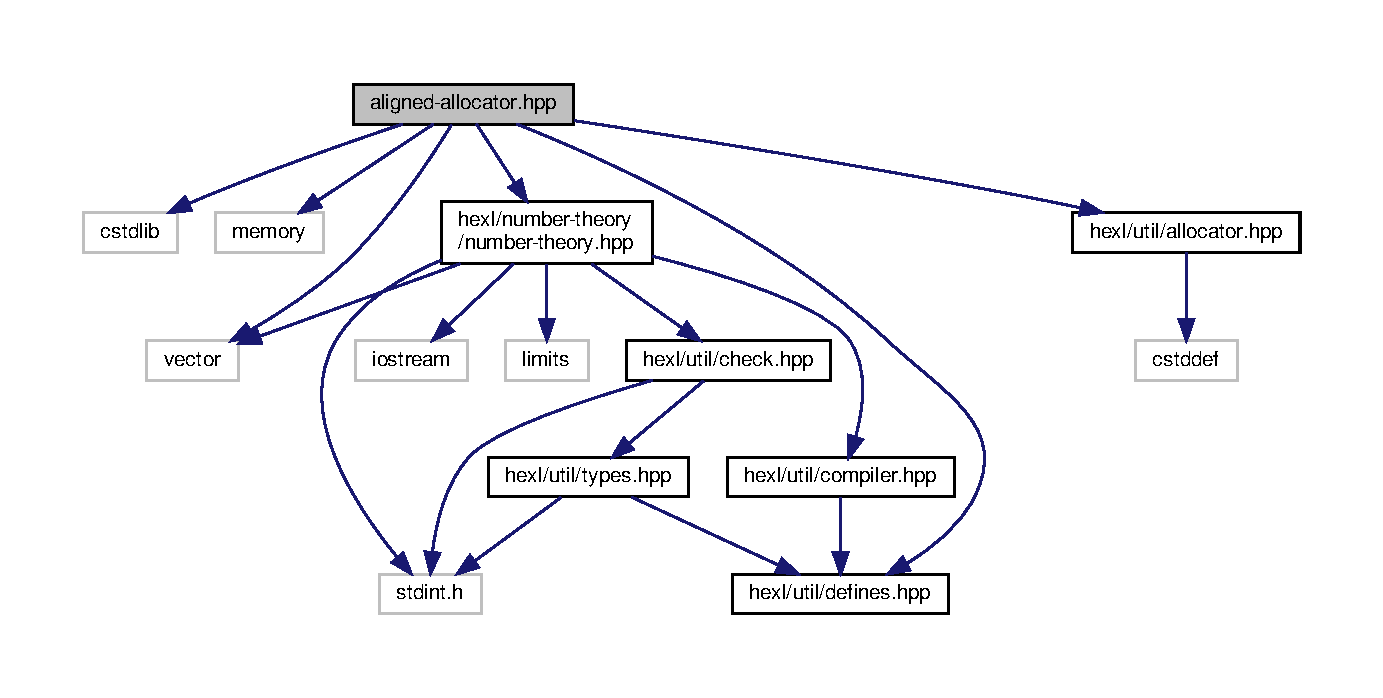
\includegraphics[width=350pt]{aligned-allocator_8hpp__incl}
\end{center}
\end{figure}
This graph shows which files directly or indirectly include this file\+:
\nopagebreak
\begin{figure}[H]
\begin{center}
\leavevmode
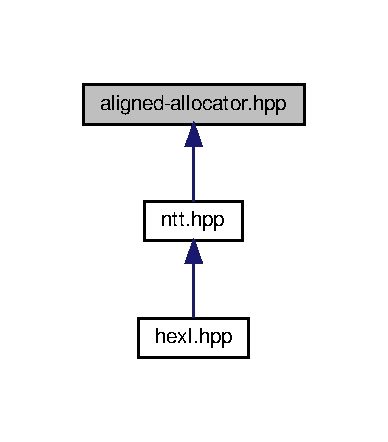
\includegraphics[width=186pt]{aligned-allocator_8hpp__dep__incl}
\end{center}
\end{figure}
\subsection*{Classes}
\begin{DoxyCompactItemize}
\item 
struct \hyperlink{structintel_1_1hexl_1_1MallocStrategy}{intel\+::hexl\+::\+Malloc\+Strategy}
\begin{DoxyCompactList}\small\item\em Allocater implementation using malloc and free. \end{DoxyCompactList}\item 
class \hyperlink{classintel_1_1hexl_1_1AlignedAllocator}{intel\+::hexl\+::\+Aligned\+Allocator$<$ T, Alignment $>$}
\begin{DoxyCompactList}\small\item\em Allocates memory aligned to Alignment-\/byte sized boundaries. \end{DoxyCompactList}\item 
struct \hyperlink{structintel_1_1hexl_1_1AlignedAllocator_1_1rebind}{intel\+::hexl\+::\+Aligned\+Allocator$<$ T, Alignment $>$\+::rebind$<$ U $>$}
\end{DoxyCompactItemize}
\subsection*{Namespaces}
\begin{DoxyCompactItemize}
\item 
 \hyperlink{namespaceintel}{intel}
\item 
 \hyperlink{namespaceintel_1_1hexl}{intel\+::hexl}
\end{DoxyCompactItemize}
\subsection*{Typedefs}
\begin{DoxyCompactItemize}
\item 
using \hyperlink{namespaceintel_1_1hexl_aced64250965d3b78827d8009634eef0c}{intel\+::hexl\+::\+Allocator\+Strategy\+Ptr} = std\+::shared\+\_\+ptr$<$ Allocator\+Base $>$
\item 
{\footnotesize template$<$typename T $>$ }\\using \hyperlink{namespaceintel_1_1hexl_afbdf0d2cc4209ee547a88ff22a02801b}{intel\+::hexl\+::\+Aligned\+Vector64} = std\+::vector$<$ T, Aligned\+Allocator$<$ T, 64 $>$ $>$
\begin{DoxyCompactList}\small\item\em 64-\/byte aligned memory allocator \end{DoxyCompactList}\end{DoxyCompactItemize}
\subsection*{Variables}
\begin{DoxyCompactItemize}
\item 
Allocator\+Strategy\+Ptr \hyperlink{namespaceintel_1_1hexl_aedc86b34ea92ac34d036acff6d84479a}{intel\+::hexl\+::malloc\+Strategy}
\end{DoxyCompactItemize}

\hypertarget{allocator_8hpp}{}\section{allocator.\+hpp File Reference}
\label{allocator_8hpp}\index{allocator.\+hpp@{allocator.\+hpp}}
{\ttfamily \#include $<$cstddef$>$}\newline
Include dependency graph for allocator.\+hpp\+:
\nopagebreak
\begin{figure}[H]
\begin{center}
\leavevmode
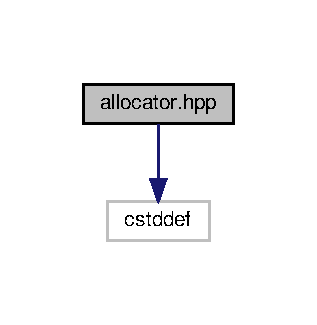
\includegraphics[width=152pt]{allocator_8hpp__incl}
\end{center}
\end{figure}
This graph shows which files directly or indirectly include this file\+:
\nopagebreak
\begin{figure}[H]
\begin{center}
\leavevmode
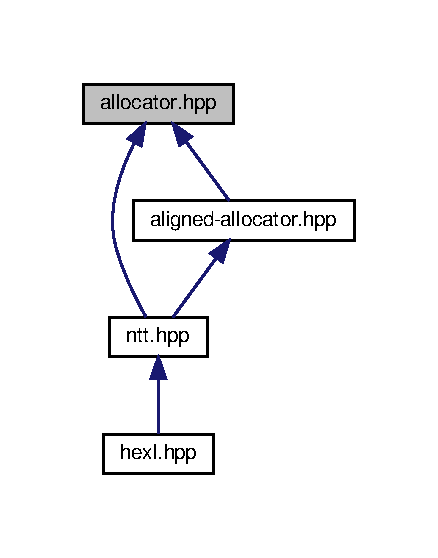
\includegraphics[width=210pt]{allocator_8hpp__dep__incl}
\end{center}
\end{figure}
\subsection*{Classes}
\begin{DoxyCompactItemize}
\item 
struct \hyperlink{structintel_1_1hexl_1_1AllocatorBase}{intel\+::hexl\+::\+Allocator\+Base}
\begin{DoxyCompactList}\small\item\em Base class for custom memory allocator. \end{DoxyCompactList}\item 
struct \hyperlink{structintel_1_1hexl_1_1AllocatorInterface}{intel\+::hexl\+::\+Allocator\+Interface$<$ Allocator\+Impl $>$}
\begin{DoxyCompactList}\small\item\em Helper memory allocation struct which delegates implementation to Allocator\+Impl. \end{DoxyCompactList}\end{DoxyCompactItemize}
\subsection*{Namespaces}
\begin{DoxyCompactItemize}
\item 
 \hyperlink{namespaceintel}{intel}
\item 
 \hyperlink{namespaceintel_1_1hexl}{intel\+::hexl}
\end{DoxyCompactItemize}

\hypertarget{check_8hpp}{}\doxysection{check.\+hpp File Reference}
\label{check_8hpp}\index{check.hpp@{check.hpp}}
{\ttfamily \#include $<$stdint.\+h$>$}\newline
{\ttfamily \#include \char`\"{}hexl/util/types.\+hpp\char`\"{}}\newline
Include dependency graph for check.\+hpp\+:
\nopagebreak
\begin{figure}[H]
\begin{center}
\leavevmode
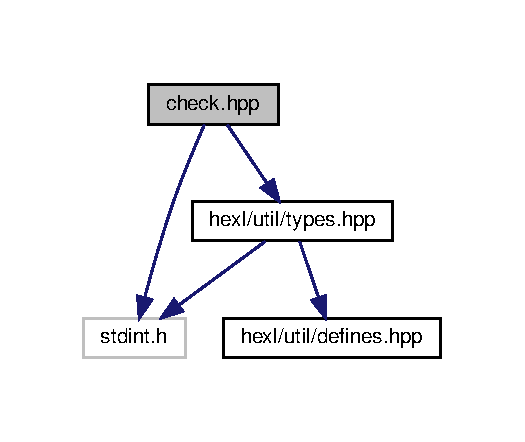
\includegraphics[width=268pt]{check_8hpp__incl}
\end{center}
\end{figure}
This graph shows which files directly or indirectly include this file\+:
\nopagebreak
\begin{figure}[H]
\begin{center}
\leavevmode
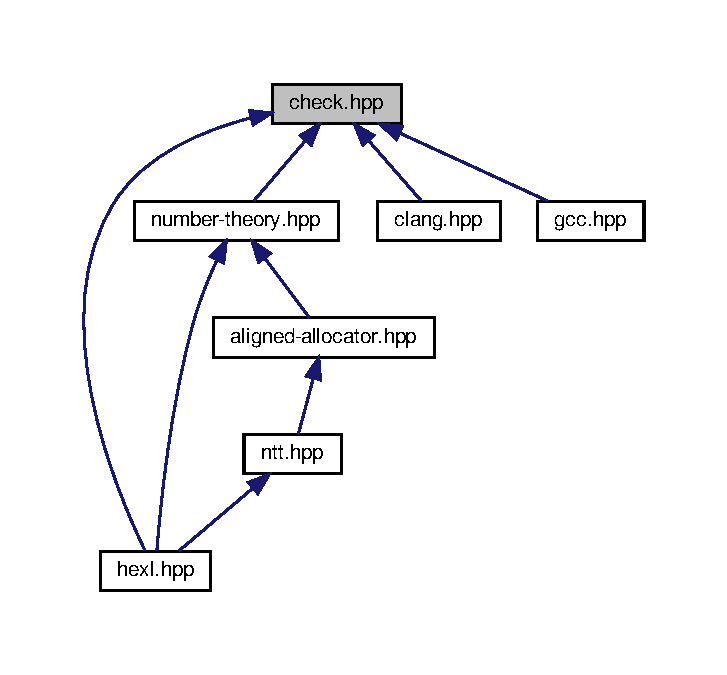
\includegraphics[width=350pt]{check_8hpp__dep__incl}
\end{center}
\end{figure}
\doxysubsection*{Macros}
\begin{DoxyCompactItemize}
\item 
\#define \mbox{\hyperlink{check_8hpp_ad5baaea0d21e2ec8c058a3de9d0f93c6}{H\+E\+X\+L\+\_\+\+C\+H\+E\+CK}}(cond,  expr)~\{\}
\item 
\#define \mbox{\hyperlink{check_8hpp_a722fda94251bc03b3a57ccdaef17abbc}{H\+E\+X\+L\+\_\+\+C\+H\+E\+C\+K\+\_\+\+B\+O\+U\+N\+DS}}(...)~\{\}
\end{DoxyCompactItemize}


\doxysubsection{Macro Definition Documentation}
\mbox{\Hypertarget{check_8hpp_ad5baaea0d21e2ec8c058a3de9d0f93c6}\label{check_8hpp_ad5baaea0d21e2ec8c058a3de9d0f93c6}} 
\index{check.hpp@{check.hpp}!HEXL\_CHECK@{HEXL\_CHECK}}
\index{HEXL\_CHECK@{HEXL\_CHECK}!check.hpp@{check.hpp}}
\doxysubsubsection{\texorpdfstring{HEXL\_CHECK}{HEXL\_CHECK}}
{\footnotesize\ttfamily \#define H\+E\+X\+L\+\_\+\+C\+H\+E\+CK(\begin{DoxyParamCaption}\item[{}]{cond,  }\item[{}]{expr }\end{DoxyParamCaption})~\{\}}

\mbox{\Hypertarget{check_8hpp_a722fda94251bc03b3a57ccdaef17abbc}\label{check_8hpp_a722fda94251bc03b3a57ccdaef17abbc}} 
\index{check.hpp@{check.hpp}!HEXL\_CHECK\_BOUNDS@{HEXL\_CHECK\_BOUNDS}}
\index{HEXL\_CHECK\_BOUNDS@{HEXL\_CHECK\_BOUNDS}!check.hpp@{check.hpp}}
\doxysubsubsection{\texorpdfstring{HEXL\_CHECK\_BOUNDS}{HEXL\_CHECK\_BOUNDS}}
{\footnotesize\ttfamily \#define H\+E\+X\+L\+\_\+\+C\+H\+E\+C\+K\+\_\+\+B\+O\+U\+N\+DS(\begin{DoxyParamCaption}\item[{}]{... }\end{DoxyParamCaption})~\{\}}


\hypertarget{ckks-multiply_8hpp}{}\doxysection{ckks-\/multiply.hpp File Reference}
\label{ckks-multiply_8hpp}\index{ckks-\/multiply.hpp@{ckks-\/multiply.hpp}}
{\ttfamily \#include $<$cstdint$>$}\newline
Include dependency graph for ckks-\/multiply.hpp\+:
\nopagebreak
\begin{figure}[H]
\begin{center}
\leavevmode
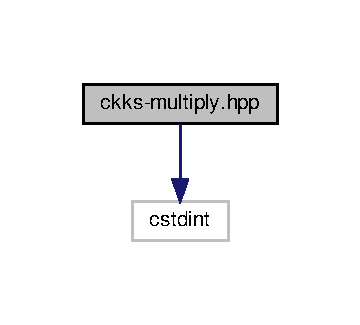
\includegraphics[width=183pt]{ckks-multiply_8hpp__incl}
\end{center}
\end{figure}
This graph shows which files directly or indirectly include this file\+:
\nopagebreak
\begin{figure}[H]
\begin{center}
\leavevmode
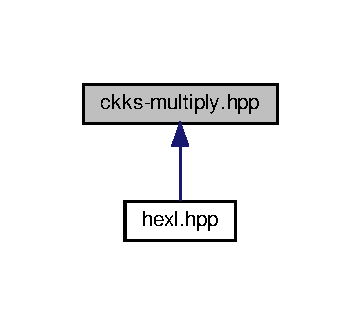
\includegraphics[width=183pt]{ckks-multiply_8hpp__dep__incl}
\end{center}
\end{figure}
\doxysubsection*{Namespaces}
\begin{DoxyCompactItemize}
\item 
 \mbox{\hyperlink{namespaceintel}{intel}}
\item 
 \mbox{\hyperlink{namespaceintel_1_1hexl}{intel\+::hexl}}
\end{DoxyCompactItemize}
\doxysubsection*{Functions}
\begin{DoxyCompactItemize}
\item 
void \mbox{\hyperlink{namespaceintel_1_1hexl_a287608abb254a6f0eeb3c7ca95e85a71}{intel\+::hexl\+::\+Ckks\+Multiply}} (uint64\+\_\+t $\ast$result, const uint64\+\_\+t $\ast$operand1, const uint64\+\_\+t $\ast$operand2, uint64\+\_\+t n, const uint64\+\_\+t $\ast$moduli, uint64\+\_\+t num\+\_\+moduli)
\begin{DoxyCompactList}\small\item\em Computes C\+K\+KS multiplication. \end{DoxyCompactList}\end{DoxyCompactItemize}

\hypertarget{ckks-switch-key_8hpp}{}\doxysection{ckks-\/switch-\/key.hpp File Reference}
\label{ckks-switch-key_8hpp}\index{ckks-\/switch-\/key.hpp@{ckks-\/switch-\/key.hpp}}
{\ttfamily \#include $<$stdint.\+h$>$}\newline
Include dependency graph for ckks-\/switch-\/key.hpp\+:
\nopagebreak
\begin{figure}[H]
\begin{center}
\leavevmode
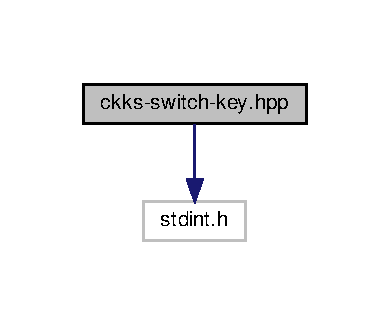
\includegraphics[width=195pt]{ckks-switch-key_8hpp__incl}
\end{center}
\end{figure}
This graph shows which files directly or indirectly include this file\+:
\nopagebreak
\begin{figure}[H]
\begin{center}
\leavevmode
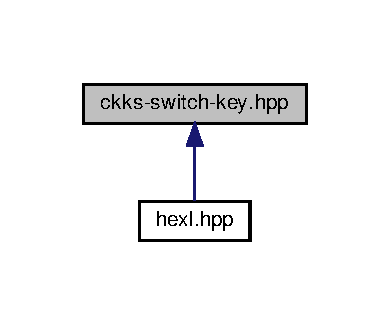
\includegraphics[width=195pt]{ckks-switch-key_8hpp__dep__incl}
\end{center}
\end{figure}
\doxysubsection*{Namespaces}
\begin{DoxyCompactItemize}
\item 
 \mbox{\hyperlink{namespaceintel}{intel}}
\item 
 \mbox{\hyperlink{namespaceintel_1_1hexl}{intel\+::hexl}}
\end{DoxyCompactItemize}
\doxysubsection*{Functions}
\begin{DoxyCompactItemize}
\item 
void \mbox{\hyperlink{namespaceintel_1_1hexl_ae983051ff4c3321db4db4569d7fbe796}{intel\+::hexl\+::\+Ckks\+Switch\+Key}} (uint64\+\_\+t $\ast$result, const uint64\+\_\+t $\ast$t\+\_\+target\+\_\+iter\+\_\+ptr, uint64\+\_\+t n, uint64\+\_\+t decomp\+\_\+modulus\+\_\+size, uint64\+\_\+t key\+\_\+modulus\+\_\+size, uint64\+\_\+t rns\+\_\+modulus\+\_\+size, uint64\+\_\+t key\+\_\+component\+\_\+count, uint64\+\_\+t $\ast$moduli, const uint64\+\_\+t $\ast$$\ast$kswitch\+\_\+keys, uint64\+\_\+t $\ast$modswitch\+\_\+factors)
\begin{DoxyCompactList}\small\item\em Computes C\+K\+KS key switching in-\/place. \end{DoxyCompactList}\end{DoxyCompactItemize}

\hypertarget{clang_8hpp}{}\doxysection{clang.\+hpp File Reference}
\label{clang_8hpp}\index{clang.hpp@{clang.hpp}}
{\ttfamily \#include $<$cmath$>$}\newline
{\ttfamily \#include \char`\"{}hexl/util/check.\+hpp\char`\"{}}\newline
{\ttfamily \#include \char`\"{}hexl/util/types.\+hpp\char`\"{}}\newline
Include dependency graph for clang.\+hpp\+:
\nopagebreak
\begin{figure}[H]
\begin{center}
\leavevmode
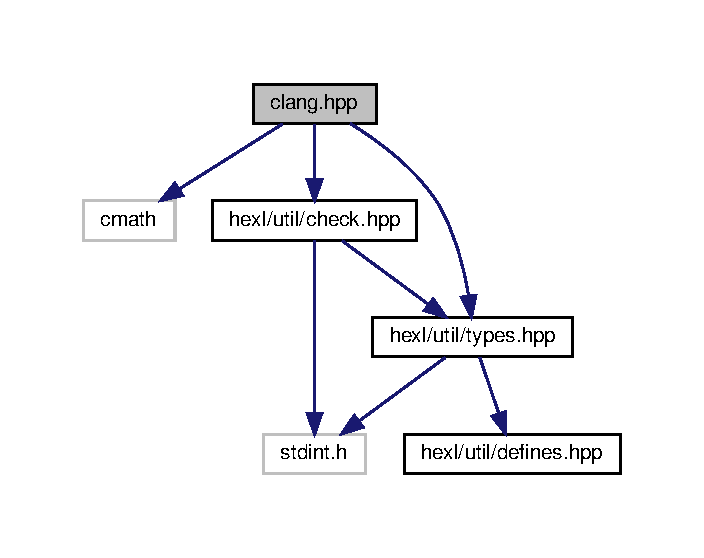
\includegraphics[width=350pt]{clang_8hpp__incl}
\end{center}
\end{figure}
\doxysubsection*{Namespaces}
\begin{DoxyCompactItemize}
\item 
 \mbox{\hyperlink{namespaceintel}{intel}}
\item 
 \mbox{\hyperlink{namespaceintel_1_1hexl}{intel\+::hexl}}
\end{DoxyCompactItemize}

\hypertarget{compiler_8hpp}{}\section{compiler.\+hpp File Reference}
\label{compiler_8hpp}\index{compiler.\+hpp@{compiler.\+hpp}}
{\ttfamily \#include \char`\"{}hexl/util/defines.\+hpp\char`\"{}}\newline
Include dependency graph for compiler.\+hpp\+:
\nopagebreak
\begin{figure}[H]
\begin{center}
\leavevmode
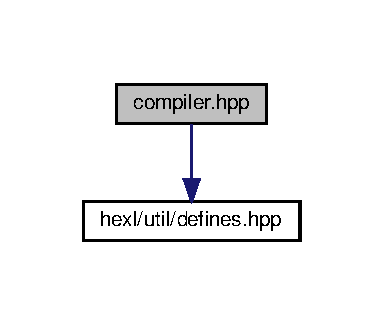
\includegraphics[width=184pt]{compiler_8hpp__incl}
\end{center}
\end{figure}
This graph shows which files directly or indirectly include this file\+:
\nopagebreak
\begin{figure}[H]
\begin{center}
\leavevmode
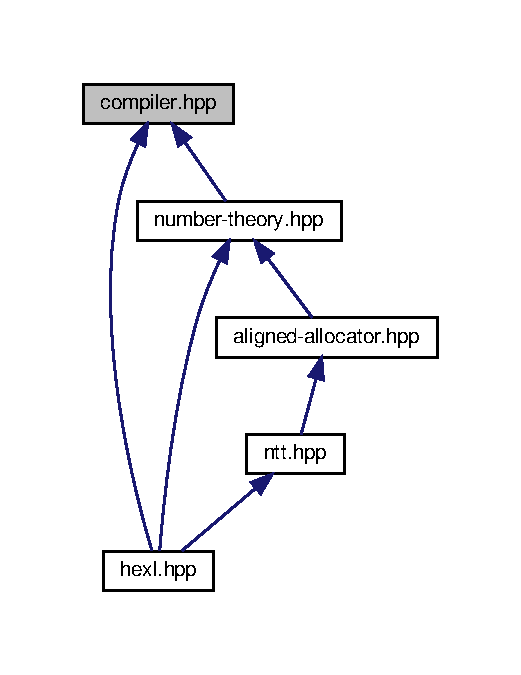
\includegraphics[width=250pt]{compiler_8hpp__dep__incl}
\end{center}
\end{figure}

\hypertarget{CONTRIBUTING_8md}{}\section{C\+O\+N\+T\+R\+I\+B\+U\+T\+I\+N\+G.\+md File Reference}
\label{CONTRIBUTING_8md}\index{C\+O\+N\+T\+R\+I\+B\+U\+T\+I\+N\+G.\+md@{C\+O\+N\+T\+R\+I\+B\+U\+T\+I\+N\+G.\+md}}

\hypertarget{defines_8hpp}{}\doxysection{defines.\+hpp File Reference}
\label{defines_8hpp}\index{defines.hpp@{defines.hpp}}
This graph shows which files directly or indirectly include this file\+:
\nopagebreak
\begin{figure}[H]
\begin{center}
\leavevmode
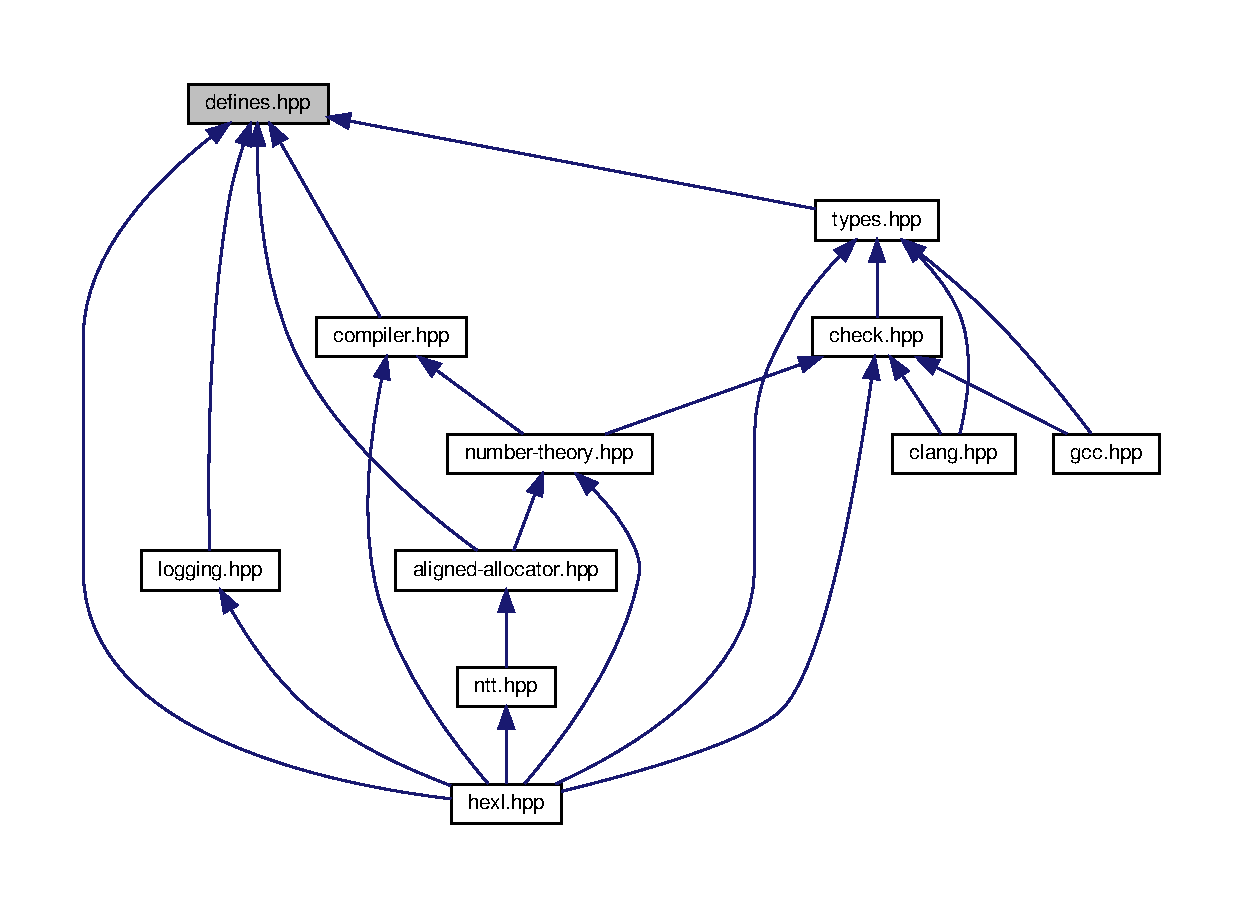
\includegraphics[width=350pt]{defines_8hpp__dep__incl}
\end{center}
\end{figure}
\doxysubsection*{Macros}
\begin{DoxyCompactItemize}
\item 
\#define \mbox{\hyperlink{defines_8hpp_a99356a2b12f66321569e4fc98fa89ac6}{H\+E\+X\+L\+\_\+\+U\+S\+E\+\_\+\+C\+L\+A\+NG}}
\end{DoxyCompactItemize}


\doxysubsection{Macro Definition Documentation}
\mbox{\Hypertarget{defines_8hpp_a99356a2b12f66321569e4fc98fa89ac6}\label{defines_8hpp_a99356a2b12f66321569e4fc98fa89ac6}} 
\index{defines.hpp@{defines.hpp}!HEXL\_USE\_CLANG@{HEXL\_USE\_CLANG}}
\index{HEXL\_USE\_CLANG@{HEXL\_USE\_CLANG}!defines.hpp@{defines.hpp}}
\doxysubsubsection{\texorpdfstring{HEXL\_USE\_CLANG}{HEXL\_USE\_CLANG}}
{\footnotesize\ttfamily \#define H\+E\+X\+L\+\_\+\+U\+S\+E\+\_\+\+C\+L\+A\+NG}


\hypertarget{eltwise-add-mod_8hpp}{}\doxysection{eltwise-\/add-\/mod.hpp File Reference}
\label{eltwise-add-mod_8hpp}\index{eltwise-\/add-\/mod.hpp@{eltwise-\/add-\/mod.hpp}}
{\ttfamily \#include $<$stdint.\+h$>$}\newline
Include dependency graph for eltwise-\/add-\/mod.hpp\+:
\nopagebreak
\begin{figure}[H]
\begin{center}
\leavevmode
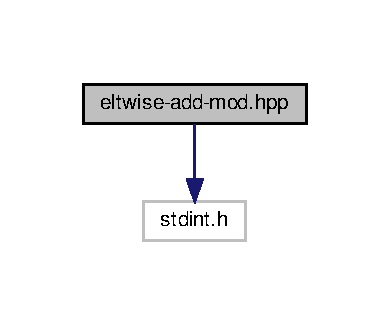
\includegraphics[width=200pt]{eltwise-add-mod_8hpp__incl}
\end{center}
\end{figure}
This graph shows which files directly or indirectly include this file\+:
\nopagebreak
\begin{figure}[H]
\begin{center}
\leavevmode
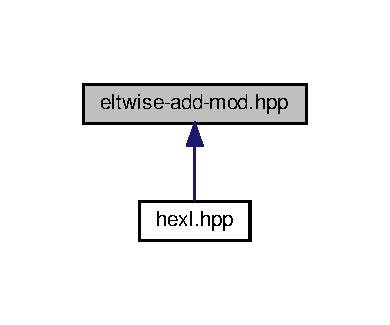
\includegraphics[width=200pt]{eltwise-add-mod_8hpp__dep__incl}
\end{center}
\end{figure}
\doxysubsection*{Namespaces}
\begin{DoxyCompactItemize}
\item 
 \mbox{\hyperlink{namespaceintel}{intel}}
\item 
 \mbox{\hyperlink{namespaceintel_1_1hexl}{intel\+::hexl}}
\end{DoxyCompactItemize}
\doxysubsection*{Functions}
\begin{DoxyCompactItemize}
\item 
void \mbox{\hyperlink{namespaceintel_1_1hexl_a319244a133f57825ba7e593ad5c71709}{intel\+::hexl\+::\+Eltwise\+Add\+Mod}} (uint64\+\_\+t $\ast$result, const uint64\+\_\+t $\ast$operand1, const uint64\+\_\+t $\ast$operand2, uint64\+\_\+t n, uint64\+\_\+t modulus)
\begin{DoxyCompactList}\small\item\em Adds two vectors elementwise with modular reduction. \end{DoxyCompactList}\item 
void \mbox{\hyperlink{namespaceintel_1_1hexl_a8e0884463658eae11b6f1c6dfeb50b40}{intel\+::hexl\+::\+Eltwise\+Add\+Mod}} (uint64\+\_\+t $\ast$result, const uint64\+\_\+t $\ast$operand1, uint64\+\_\+t operand2, uint64\+\_\+t n, uint64\+\_\+t modulus)
\begin{DoxyCompactList}\small\item\em Adds a vector and scalar elementwise with modular reduction. \end{DoxyCompactList}\end{DoxyCompactItemize}

\hypertarget{eltwise-cmp-add_8hpp}{}\doxysection{eltwise-\/cmp-\/add.hpp File Reference}
\label{eltwise-cmp-add_8hpp}\index{eltwise-\/cmp-\/add.hpp@{eltwise-\/cmp-\/add.hpp}}
{\ttfamily \#include $<$stdint.\+h$>$}\newline
{\ttfamily \#include \char`\"{}hexl/util/util.\+hpp\char`\"{}}\newline
Include dependency graph for eltwise-\/cmp-\/add.hpp\+:
\nopagebreak
\begin{figure}[H]
\begin{center}
\leavevmode
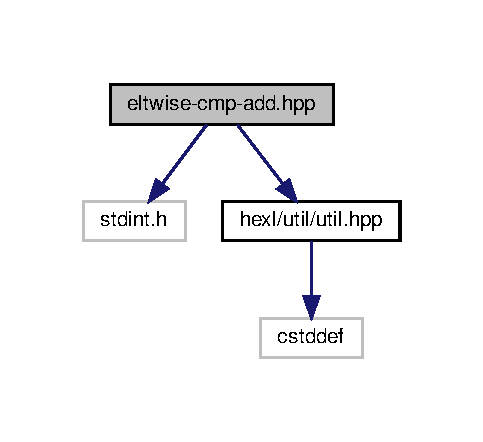
\includegraphics[width=248pt]{eltwise-cmp-add_8hpp__incl}
\end{center}
\end{figure}
This graph shows which files directly or indirectly include this file\+:
\nopagebreak
\begin{figure}[H]
\begin{center}
\leavevmode
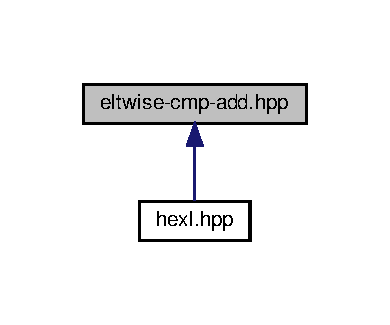
\includegraphics[width=199pt]{eltwise-cmp-add_8hpp__dep__incl}
\end{center}
\end{figure}
\doxysubsection*{Namespaces}
\begin{DoxyCompactItemize}
\item 
 \mbox{\hyperlink{namespaceintel}{intel}}
\item 
 \mbox{\hyperlink{namespaceintel_1_1hexl}{intel\+::hexl}}
\end{DoxyCompactItemize}
\doxysubsection*{Functions}
\begin{DoxyCompactItemize}
\item 
void \mbox{\hyperlink{namespaceintel_1_1hexl_a5c4fd2ceb53b94efa5f5a959d7ee9819}{intel\+::hexl\+::\+Eltwise\+Cmp\+Add}} (uint64\+\_\+t $\ast$result, const uint64\+\_\+t $\ast$operand1, uint64\+\_\+t n, C\+M\+P\+I\+NT cmp, uint64\+\_\+t bound, uint64\+\_\+t diff)
\begin{DoxyCompactList}\small\item\em Computes element-\/wise conditional addition. \end{DoxyCompactList}\end{DoxyCompactItemize}

\hypertarget{eltwise-cmp-sub-mod_8hpp}{}\doxysection{eltwise-\/cmp-\/sub-\/mod.hpp File Reference}
\label{eltwise-cmp-sub-mod_8hpp}\index{eltwise-\/cmp-\/sub-\/mod.hpp@{eltwise-\/cmp-\/sub-\/mod.hpp}}
{\ttfamily \#include $<$stdint.\+h$>$}\newline
{\ttfamily \#include \char`\"{}hexl/util/util.\+hpp\char`\"{}}\newline
Include dependency graph for eltwise-\/cmp-\/sub-\/mod.hpp\+:
\nopagebreak
\begin{figure}[H]
\begin{center}
\leavevmode
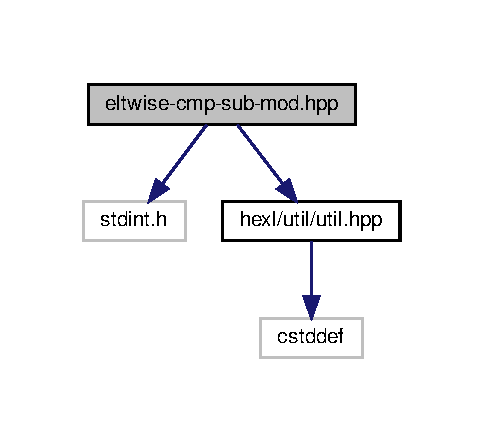
\includegraphics[width=248pt]{eltwise-cmp-sub-mod_8hpp__incl}
\end{center}
\end{figure}
This graph shows which files directly or indirectly include this file\+:
\nopagebreak
\begin{figure}[H]
\begin{center}
\leavevmode
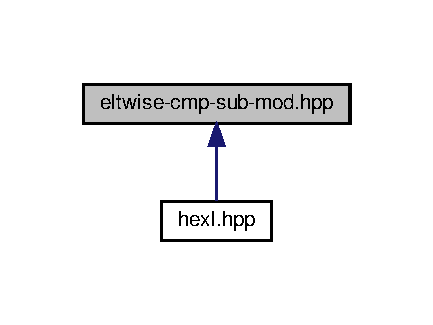
\includegraphics[width=224pt]{eltwise-cmp-sub-mod_8hpp__dep__incl}
\end{center}
\end{figure}
\doxysubsection*{Namespaces}
\begin{DoxyCompactItemize}
\item 
 \mbox{\hyperlink{namespaceintel}{intel}}
\item 
 \mbox{\hyperlink{namespaceintel_1_1hexl}{intel\+::hexl}}
\end{DoxyCompactItemize}
\doxysubsection*{Functions}
\begin{DoxyCompactItemize}
\item 
void \mbox{\hyperlink{namespaceintel_1_1hexl_a78bf86d32140e39d8f99d474ccd0e226}{intel\+::hexl\+::\+Eltwise\+Cmp\+Sub\+Mod}} (uint64\+\_\+t $\ast$result, const uint64\+\_\+t $\ast$operand1, uint64\+\_\+t n, uint64\+\_\+t modulus, C\+M\+P\+I\+NT cmp, uint64\+\_\+t bound, uint64\+\_\+t diff)
\begin{DoxyCompactList}\small\item\em Computes element-\/wise conditional modular subtraction. \end{DoxyCompactList}\end{DoxyCompactItemize}

\hypertarget{eltwise-fma-mod_8hpp}{}\section{eltwise-\/fma-\/mod.hpp File Reference}
\label{eltwise-fma-mod_8hpp}\index{eltwise-\/fma-\/mod.\+hpp@{eltwise-\/fma-\/mod.\+hpp}}
{\ttfamily \#include $<$stdint.\+h$>$}\newline
Include dependency graph for eltwise-\/fma-\/mod.hpp\+:
\nopagebreak
\begin{figure}[H]
\begin{center}
\leavevmode
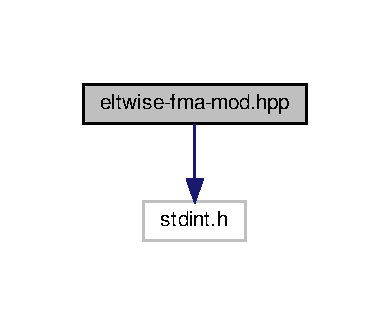
\includegraphics[width=187pt]{eltwise-fma-mod_8hpp__incl}
\end{center}
\end{figure}
This graph shows which files directly or indirectly include this file\+:
\nopagebreak
\begin{figure}[H]
\begin{center}
\leavevmode
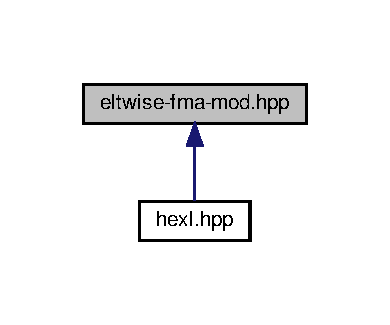
\includegraphics[width=187pt]{eltwise-fma-mod_8hpp__dep__incl}
\end{center}
\end{figure}
\subsection*{Namespaces}
\begin{DoxyCompactItemize}
\item 
 \hyperlink{namespaceintel}{intel}
\item 
 \hyperlink{namespaceintel_1_1hexl}{intel\+::hexl}
\end{DoxyCompactItemize}
\subsection*{Functions}
\begin{DoxyCompactItemize}
\item 
void \hyperlink{namespaceintel_1_1hexl_a5b65d563391b4a1a5041633aeb118aa5}{intel\+::hexl\+::\+Eltwise\+F\+M\+A\+Mod} (uint64\+\_\+t $\ast$result, const uint64\+\_\+t $\ast$arg1, uint64\+\_\+t arg2, const uint64\+\_\+t $\ast$arg3, uint64\+\_\+t n, uint64\+\_\+t modulus, uint64\+\_\+t input\+\_\+mod\+\_\+factor)
\begin{DoxyCompactList}\small\item\em Computes fused multiply-\/add ({\ttfamily arg1} $\ast$ {\ttfamily arg2} + {\ttfamily arg3}) mod {\ttfamily modulus} element-\/wise, broadcasting scalars to vectors. \end{DoxyCompactList}\end{DoxyCompactItemize}

\hypertarget{eltwise-mult-mod_8hpp}{}\section{eltwise-\/mult-\/mod.hpp File Reference}
\label{eltwise-mult-mod_8hpp}\index{eltwise-\/mult-\/mod.\+hpp@{eltwise-\/mult-\/mod.\+hpp}}
{\ttfamily \#include $<$stdint.\+h$>$}\newline
Include dependency graph for eltwise-\/mult-\/mod.hpp\+:
\nopagebreak
\begin{figure}[H]
\begin{center}
\leavevmode
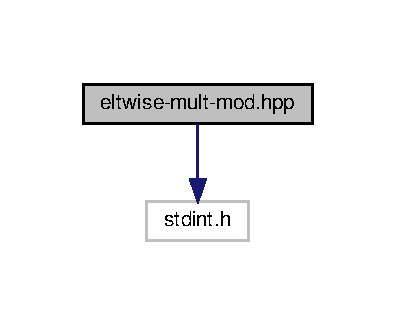
\includegraphics[width=190pt]{eltwise-mult-mod_8hpp__incl}
\end{center}
\end{figure}
This graph shows which files directly or indirectly include this file\+:
\nopagebreak
\begin{figure}[H]
\begin{center}
\leavevmode
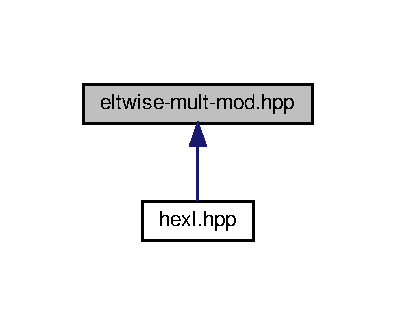
\includegraphics[width=190pt]{eltwise-mult-mod_8hpp__dep__incl}
\end{center}
\end{figure}
\subsection*{Namespaces}
\begin{DoxyCompactItemize}
\item 
 \hyperlink{namespaceintel}{intel}
\item 
 \hyperlink{namespaceintel_1_1hexl}{intel\+::hexl}
\end{DoxyCompactItemize}
\subsection*{Functions}
\begin{DoxyCompactItemize}
\item 
void \hyperlink{namespaceintel_1_1hexl_a705bc0321d937ae4d1f8d50279e3cff1}{intel\+::hexl\+::\+Eltwise\+Mult\+Mod} (uint64\+\_\+t $\ast$result, const uint64\+\_\+t $\ast$operand1, const uint64\+\_\+t $\ast$operand2, uint64\+\_\+t n, uint64\+\_\+t modulus, uint64\+\_\+t input\+\_\+mod\+\_\+factor)
\begin{DoxyCompactList}\small\item\em Multiplies two vectors elementwise with modular reduction. \end{DoxyCompactList}\end{DoxyCompactItemize}

\hypertarget{eltwise-reduce-mod_8hpp}{}\section{eltwise-\/reduce-\/mod.hpp File Reference}
\label{eltwise-reduce-mod_8hpp}\index{eltwise-\/reduce-\/mod.\+hpp@{eltwise-\/reduce-\/mod.\+hpp}}
{\ttfamily \#include $<$stdint.\+h$>$}\newline
Include dependency graph for eltwise-\/reduce-\/mod.hpp\+:
\nopagebreak
\begin{figure}[H]
\begin{center}
\leavevmode
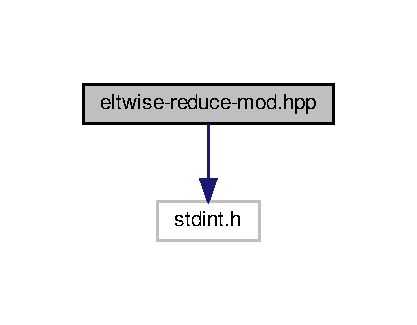
\includegraphics[width=200pt]{eltwise-reduce-mod_8hpp__incl}
\end{center}
\end{figure}
This graph shows which files directly or indirectly include this file\+:
\nopagebreak
\begin{figure}[H]
\begin{center}
\leavevmode
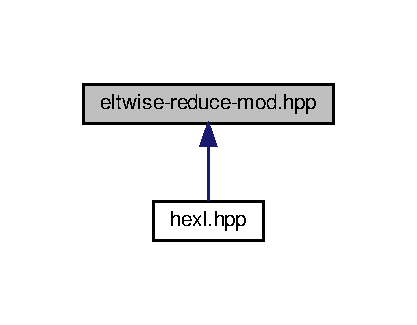
\includegraphics[width=200pt]{eltwise-reduce-mod_8hpp__dep__incl}
\end{center}
\end{figure}
\subsection*{Namespaces}
\begin{DoxyCompactItemize}
\item 
 \hyperlink{namespaceintel}{intel}
\item 
 \hyperlink{namespaceintel_1_1hexl}{intel\+::hexl}
\end{DoxyCompactItemize}
\subsection*{Functions}
\begin{DoxyCompactItemize}
\item 
void \hyperlink{namespaceintel_1_1hexl_af3ddae165283841d495a322275baf5ee}{intel\+::hexl\+::\+Eltwise\+Reduce\+Mod} (uint64\+\_\+t $\ast$result, const uint64\+\_\+t $\ast$operand, uint64\+\_\+t n, uint64\+\_\+t modulus, uint64\+\_\+t input\+\_\+mod\+\_\+factor, uint64\+\_\+t output\+\_\+mod\+\_\+factor)
\begin{DoxyCompactList}\small\item\em Performs elementwise modular reduction. \end{DoxyCompactList}\end{DoxyCompactItemize}

\hypertarget{eltwise-sub-mod_8hpp}{}\doxysection{eltwise-\/sub-\/mod.hpp File Reference}
\label{eltwise-sub-mod_8hpp}\index{eltwise-\/sub-\/mod.hpp@{eltwise-\/sub-\/mod.hpp}}
{\ttfamily \#include $<$stdint.\+h$>$}\newline
Include dependency graph for eltwise-\/sub-\/mod.hpp\+:
\nopagebreak
\begin{figure}[H]
\begin{center}
\leavevmode
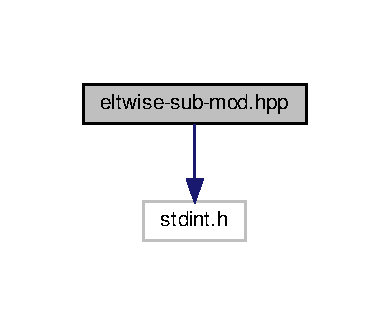
\includegraphics[width=199pt]{eltwise-sub-mod_8hpp__incl}
\end{center}
\end{figure}
This graph shows which files directly or indirectly include this file\+:
\nopagebreak
\begin{figure}[H]
\begin{center}
\leavevmode
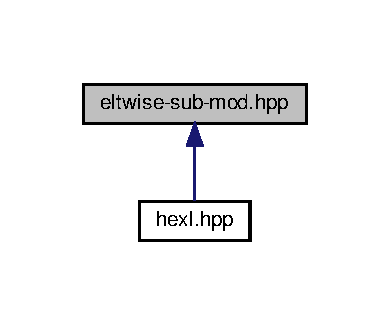
\includegraphics[width=199pt]{eltwise-sub-mod_8hpp__dep__incl}
\end{center}
\end{figure}
\doxysubsection*{Namespaces}
\begin{DoxyCompactItemize}
\item 
 \mbox{\hyperlink{namespaceintel}{intel}}
\item 
 \mbox{\hyperlink{namespaceintel_1_1hexl}{intel\+::hexl}}
\end{DoxyCompactItemize}
\doxysubsection*{Functions}
\begin{DoxyCompactItemize}
\item 
void \mbox{\hyperlink{namespaceintel_1_1hexl_a6a45c30bc21b9b1e1410b23fce5424c8}{intel\+::hexl\+::\+Eltwise\+Sub\+Mod}} (uint64\+\_\+t $\ast$result, const uint64\+\_\+t $\ast$operand1, const uint64\+\_\+t $\ast$operand2, uint64\+\_\+t n, uint64\+\_\+t modulus)
\begin{DoxyCompactList}\small\item\em Subtracts two vectors elementwise with modular reduction. \end{DoxyCompactList}\item 
void \mbox{\hyperlink{namespaceintel_1_1hexl_abc13b8f383d3af6471a5261ee2213b40}{intel\+::hexl\+::\+Eltwise\+Sub\+Mod}} (uint64\+\_\+t $\ast$result, const uint64\+\_\+t $\ast$operand1, uint64\+\_\+t operand2, uint64\+\_\+t n, uint64\+\_\+t modulus)
\begin{DoxyCompactList}\small\item\em Subtracts a scalar from a vector elementwise with modular reduction. \end{DoxyCompactList}\end{DoxyCompactItemize}

\hypertarget{gcc_8hpp}{}\doxysection{gcc.\+hpp File Reference}
\label{gcc_8hpp}\index{gcc.hpp@{gcc.hpp}}
{\ttfamily \#include $<$cmath$>$}\newline
{\ttfamily \#include \char`\"{}hexl/util/check.\+hpp\char`\"{}}\newline
{\ttfamily \#include \char`\"{}hexl/util/types.\+hpp\char`\"{}}\newline
Include dependency graph for gcc.\+hpp\+:
\nopagebreak
\begin{figure}[H]
\begin{center}
\leavevmode
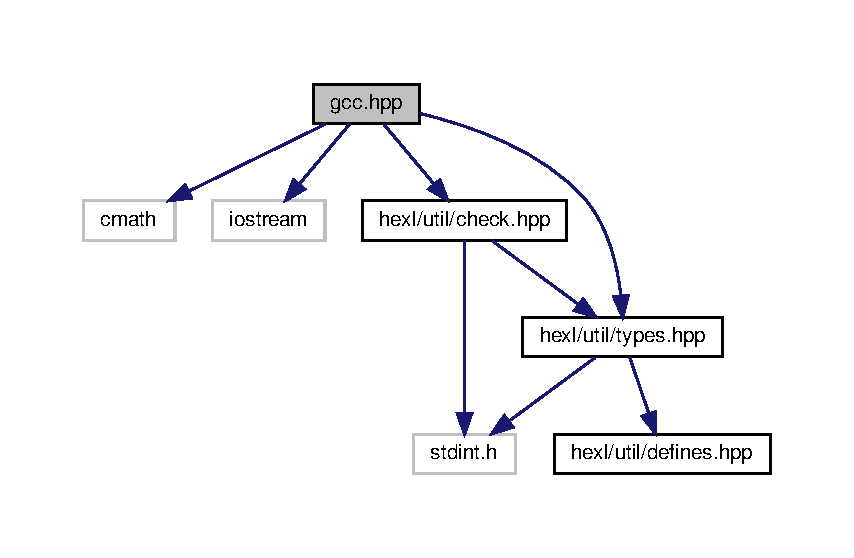
\includegraphics[width=350pt]{gcc_8hpp__incl}
\end{center}
\end{figure}
\doxysubsection*{Namespaces}
\begin{DoxyCompactItemize}
\item 
 \mbox{\hyperlink{namespaceintel}{intel}}
\item 
 \mbox{\hyperlink{namespaceintel_1_1hexl}{intel\+::hexl}}
\end{DoxyCompactItemize}

\hypertarget{hexl_8hpp}{}\doxysection{hexl.\+hpp File Reference}
\label{hexl_8hpp}\index{hexl.hpp@{hexl.hpp}}
{\ttfamily \#include \char`\"{}hexl/eltwise/eltwise-\/add-\/mod.\+hpp\char`\"{}}\newline
{\ttfamily \#include \char`\"{}hexl/eltwise/eltwise-\/cmp-\/add.\+hpp\char`\"{}}\newline
{\ttfamily \#include \char`\"{}hexl/eltwise/eltwise-\/cmp-\/sub-\/mod.\+hpp\char`\"{}}\newline
{\ttfamily \#include \char`\"{}hexl/eltwise/eltwise-\/fma-\/mod.\+hpp\char`\"{}}\newline
{\ttfamily \#include \char`\"{}hexl/eltwise/eltwise-\/mult-\/mod.\+hpp\char`\"{}}\newline
{\ttfamily \#include \char`\"{}hexl/eltwise/eltwise-\/reduce-\/mod.\+hpp\char`\"{}}\newline
{\ttfamily \#include \char`\"{}hexl/eltwise/eltwise-\/sub-\/mod.\+hpp\char`\"{}}\newline
{\ttfamily \#include \char`\"{}hexl/experimental/seal/ckks-\/multiply.\+hpp\char`\"{}}\newline
{\ttfamily \#include \char`\"{}hexl/experimental/seal/ckks-\/switch-\/key.\+hpp\char`\"{}}\newline
{\ttfamily \#include \char`\"{}hexl/logging/logging.\+hpp\char`\"{}}\newline
{\ttfamily \#include \char`\"{}hexl/ntt/ntt.\+hpp\char`\"{}}\newline
{\ttfamily \#include \char`\"{}hexl/number-\/theory/number-\/theory.\+hpp\char`\"{}}\newline
{\ttfamily \#include \char`\"{}hexl/util/check.\+hpp\char`\"{}}\newline
{\ttfamily \#include \char`\"{}hexl/util/compiler.\+hpp\char`\"{}}\newline
{\ttfamily \#include \char`\"{}hexl/util/defines.\+hpp\char`\"{}}\newline
{\ttfamily \#include \char`\"{}hexl/util/types.\+hpp\char`\"{}}\newline
{\ttfamily \#include \char`\"{}hexl/util/util.\+hpp\char`\"{}}\newline
Include dependency graph for hexl.\+hpp\+:
\nopagebreak
\begin{figure}[H]
\begin{center}
\leavevmode
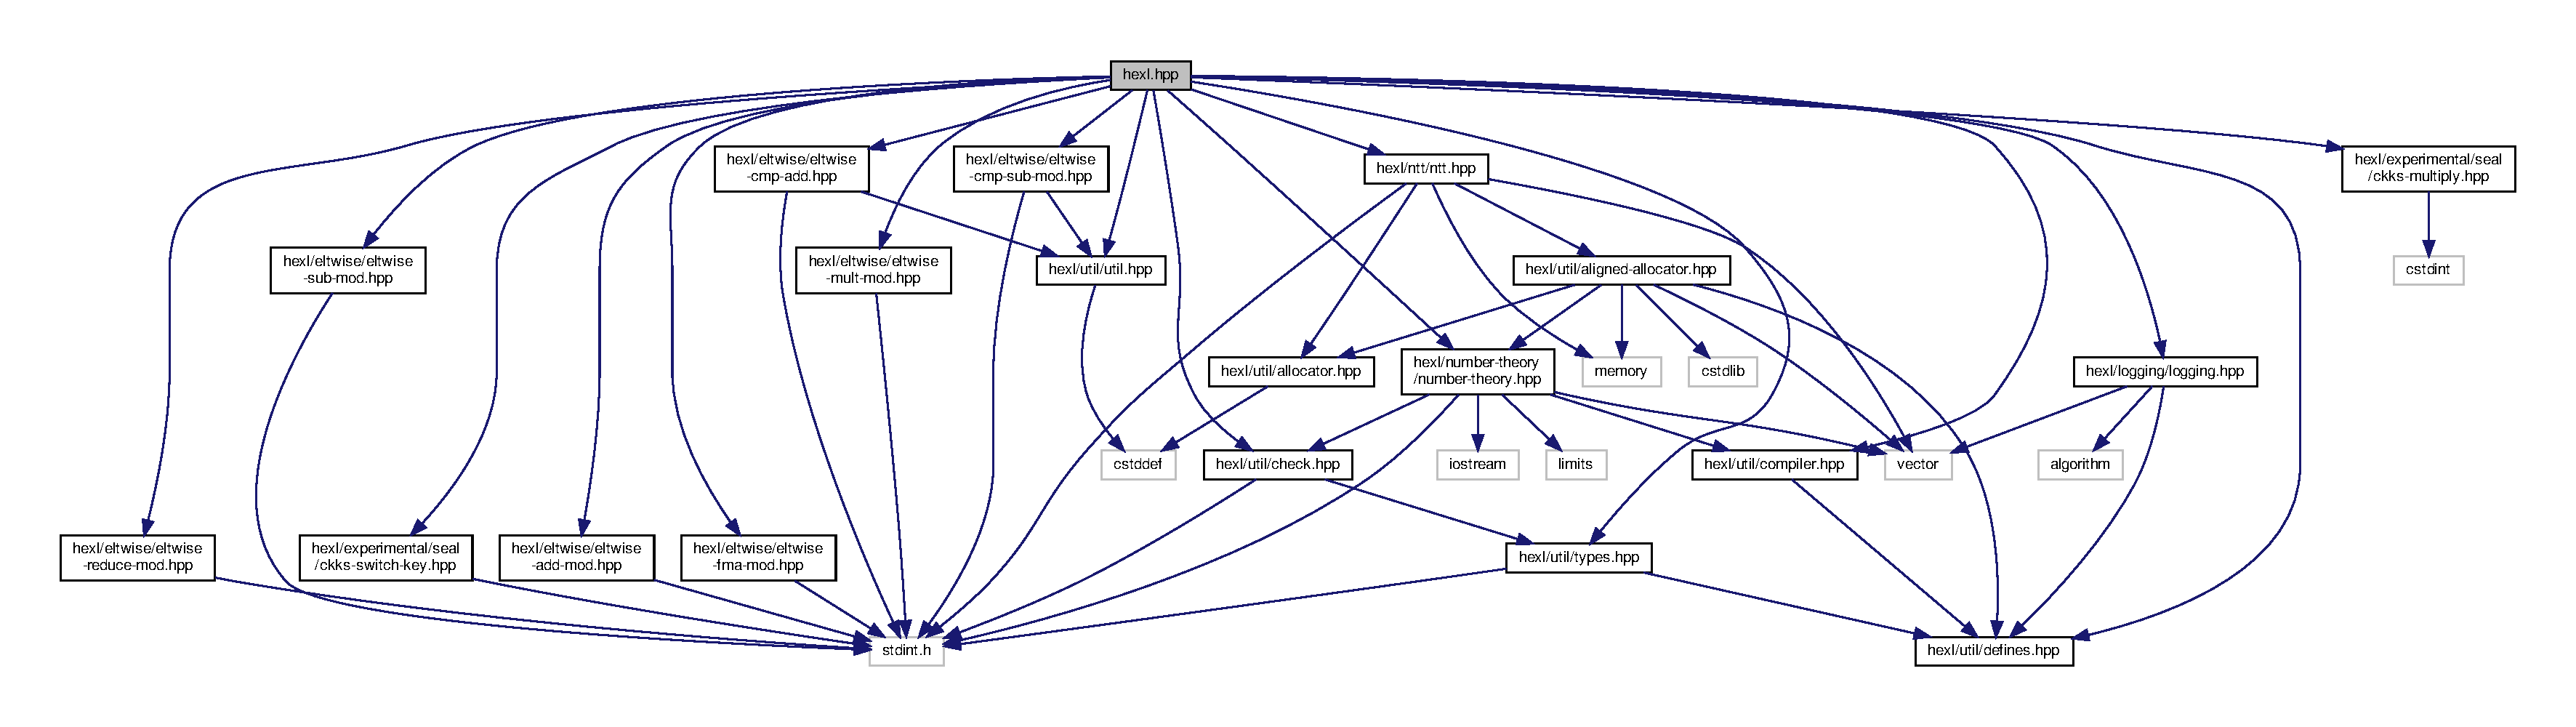
\includegraphics[width=350pt]{hexl_8hpp__incl}
\end{center}
\end{figure}

\hypertarget{logging_8hpp}{}\doxysection{logging.\+hpp File Reference}
\label{logging_8hpp}\index{logging.hpp@{logging.hpp}}
{\ttfamily \#include $<$algorithm$>$}\newline
{\ttfamily \#include $<$vector$>$}\newline
{\ttfamily \#include \char`\"{}hexl/util/defines.\+hpp\char`\"{}}\newline
Include dependency graph for logging.\+hpp\+:
\nopagebreak
\begin{figure}[H]
\begin{center}
\leavevmode
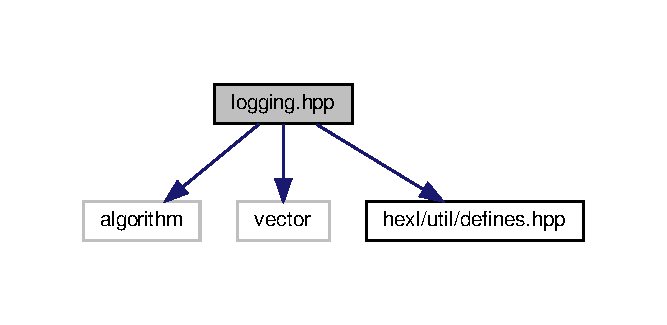
\includegraphics[width=344pt]{logging_8hpp__incl}
\end{center}
\end{figure}
This graph shows which files directly or indirectly include this file\+:
\nopagebreak
\begin{figure}[H]
\begin{center}
\leavevmode
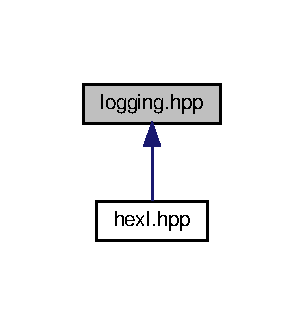
\includegraphics[width=154pt]{logging_8hpp__dep__incl}
\end{center}
\end{figure}
\doxysubsection*{Macros}
\begin{DoxyCompactItemize}
\item 
\#define \mbox{\hyperlink{logging_8hpp_af5370a040d5e43db53a00e6126ca189c}{H\+E\+X\+L\+\_\+\+V\+L\+OG}}(N,  rest)~\{\}
\item 
\#define \mbox{\hyperlink{logging_8hpp_a9382a5697af55d4985fc5697efcd494c}{S\+T\+A\+R\+T\+\_\+\+E\+A\+S\+Y\+L\+O\+G\+G\+I\+N\+G\+PP}}(X,  Y)~\{\}
\end{DoxyCompactItemize}


\doxysubsection{Macro Definition Documentation}
\mbox{\Hypertarget{logging_8hpp_af5370a040d5e43db53a00e6126ca189c}\label{logging_8hpp_af5370a040d5e43db53a00e6126ca189c}} 
\index{logging.hpp@{logging.hpp}!HEXL\_VLOG@{HEXL\_VLOG}}
\index{HEXL\_VLOG@{HEXL\_VLOG}!logging.hpp@{logging.hpp}}
\doxysubsubsection{\texorpdfstring{HEXL\_VLOG}{HEXL\_VLOG}}
{\footnotesize\ttfamily \#define H\+E\+X\+L\+\_\+\+V\+L\+OG(\begin{DoxyParamCaption}\item[{}]{N,  }\item[{}]{rest }\end{DoxyParamCaption})~\{\}}

\mbox{\Hypertarget{logging_8hpp_a9382a5697af55d4985fc5697efcd494c}\label{logging_8hpp_a9382a5697af55d4985fc5697efcd494c}} 
\index{logging.hpp@{logging.hpp}!START\_EASYLOGGINGPP@{START\_EASYLOGGINGPP}}
\index{START\_EASYLOGGINGPP@{START\_EASYLOGGINGPP}!logging.hpp@{logging.hpp}}
\doxysubsubsection{\texorpdfstring{START\_EASYLOGGINGPP}{START\_EASYLOGGINGPP}}
{\footnotesize\ttfamily \#define S\+T\+A\+R\+T\+\_\+\+E\+A\+S\+Y\+L\+O\+G\+G\+I\+N\+G\+PP(\begin{DoxyParamCaption}\item[{}]{X,  }\item[{}]{Y }\end{DoxyParamCaption})~\{\}}


\hypertarget{msvc_8hpp}{}\doxysection{msvc.\+hpp File Reference}
\label{msvc_8hpp}\index{msvc.hpp@{msvc.hpp}}

\hypertarget{ntt_8hpp}{}\doxysection{ntt.\+hpp File Reference}
\label{ntt_8hpp}\index{ntt.hpp@{ntt.hpp}}
{\ttfamily \#include $<$stdint.\+h$>$}\newline
{\ttfamily \#include $<$memory$>$}\newline
{\ttfamily \#include $<$vector$>$}\newline
{\ttfamily \#include \char`\"{}hexl/util/aligned-\/allocator.\+hpp\char`\"{}}\newline
{\ttfamily \#include \char`\"{}hexl/util/allocator.\+hpp\char`\"{}}\newline
Include dependency graph for ntt.\+hpp\+:
\nopagebreak
\begin{figure}[H]
\begin{center}
\leavevmode
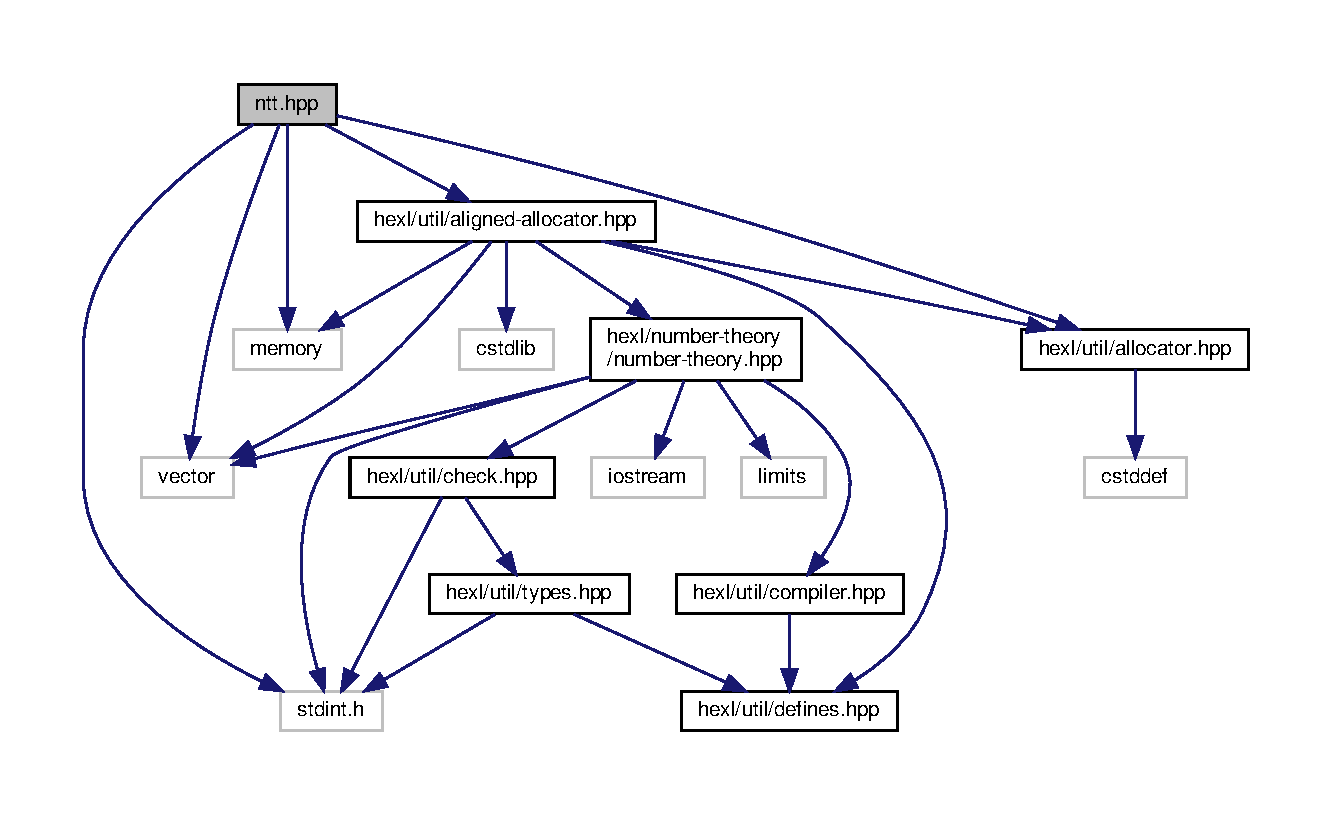
\includegraphics[width=350pt]{ntt_8hpp__incl}
\end{center}
\end{figure}
This graph shows which files directly or indirectly include this file\+:
\nopagebreak
\begin{figure}[H]
\begin{center}
\leavevmode
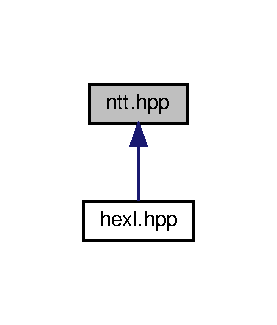
\includegraphics[width=139pt]{ntt_8hpp__dep__incl}
\end{center}
\end{figure}
\doxysubsection*{Classes}
\begin{DoxyCompactItemize}
\item 
class \mbox{\hyperlink{classintel_1_1hexl_1_1NTT}{intel\+::hexl\+::\+N\+TT}}
\begin{DoxyCompactList}\small\item\em Performs negacyclic forward and inverse number-\/theoretic transform (\mbox{\hyperlink{classintel_1_1hexl_1_1NTT}{N\+TT}}), commonly used in R\+L\+WE cryptography. \end{DoxyCompactList}\item 
struct \mbox{\hyperlink{structintel_1_1hexl_1_1NTT_1_1AllocatorAdapter}{intel\+::hexl\+::\+N\+T\+T\+::\+Allocator\+Adapter$<$ Adaptee, Args $>$}}
\begin{DoxyCompactList}\small\item\em Helper class for custom memory allocation. \end{DoxyCompactList}\end{DoxyCompactItemize}
\doxysubsection*{Namespaces}
\begin{DoxyCompactItemize}
\item 
 \mbox{\hyperlink{namespaceintel}{intel}}
\item 
 \mbox{\hyperlink{namespaceintel_1_1hexl}{intel\+::hexl}}
\end{DoxyCompactItemize}

\hypertarget{number-theory_8hpp}{}\section{number-\/theory.hpp File Reference}
\label{number-theory_8hpp}\index{number-\/theory.\+hpp@{number-\/theory.\+hpp}}
{\ttfamily \#include $<$stdint.\+h$>$}\newline
{\ttfamily \#include $<$iostream$>$}\newline
{\ttfamily \#include $<$limits$>$}\newline
{\ttfamily \#include $<$vector$>$}\newline
{\ttfamily \#include \char`\"{}hexl/util/check.\+hpp\char`\"{}}\newline
{\ttfamily \#include \char`\"{}hexl/util/compiler.\+hpp\char`\"{}}\newline
Include dependency graph for number-\/theory.hpp\+:
\nopagebreak
\begin{figure}[H]
\begin{center}
\leavevmode
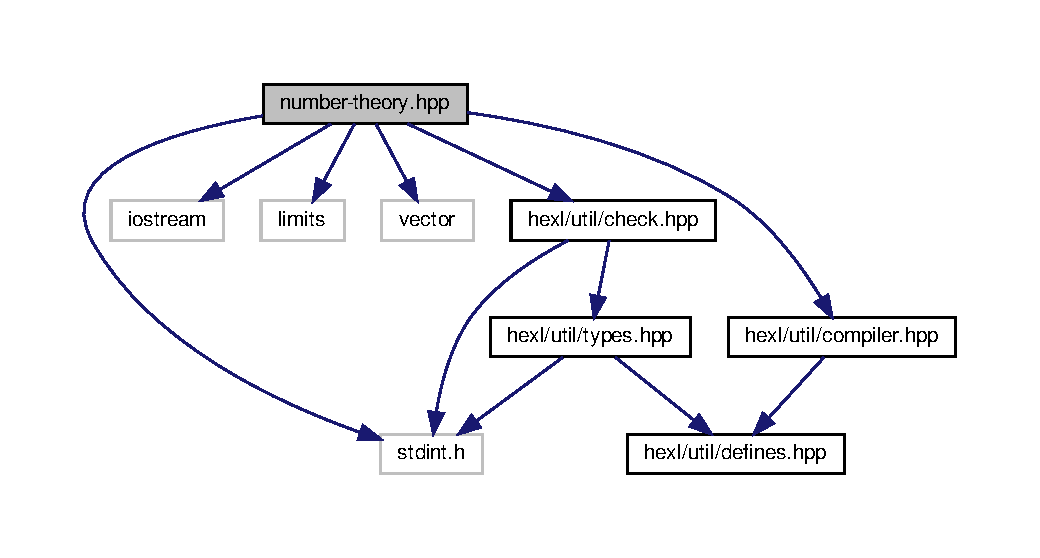
\includegraphics[width=350pt]{number-theory_8hpp__incl}
\end{center}
\end{figure}
This graph shows which files directly or indirectly include this file\+:
\nopagebreak
\begin{figure}[H]
\begin{center}
\leavevmode
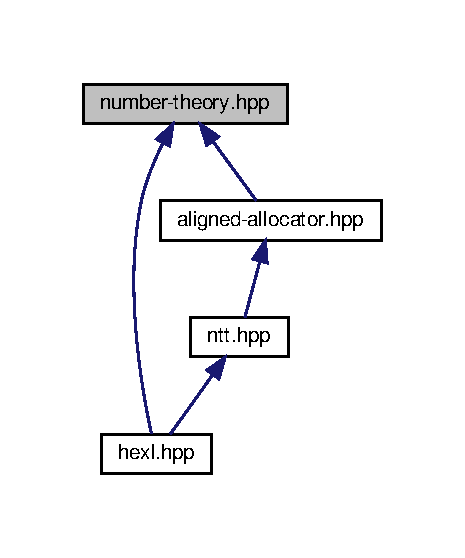
\includegraphics[width=223pt]{number-theory_8hpp__dep__incl}
\end{center}
\end{figure}
\subsection*{Classes}
\begin{DoxyCompactItemize}
\item 
class \hyperlink{classintel_1_1hexl_1_1MultiplyFactor}{intel\+::hexl\+::\+Multiply\+Factor}
\begin{DoxyCompactList}\small\item\em Pre-\/computes a Barrett factor with which modular multiplication can be performed more efficiently. \end{DoxyCompactList}\end{DoxyCompactItemize}
\subsection*{Namespaces}
\begin{DoxyCompactItemize}
\item 
 \hyperlink{namespaceintel}{intel}
\item 
 \hyperlink{namespaceintel_1_1hexl}{intel\+::hexl}
\end{DoxyCompactItemize}
\subsection*{Functions}
\begin{DoxyCompactItemize}
\item 
bool \hyperlink{namespaceintel_1_1hexl_ada0fe74afb4384b54728cba8ec3f69cd}{intel\+::hexl\+::\+Is\+Power\+Of\+Two} (uint64\+\_\+t num)
\begin{DoxyCompactList}\small\item\em Returns whether or not num is a power of two. \end{DoxyCompactList}\item 
uint64\+\_\+t \hyperlink{namespaceintel_1_1hexl_a066a83a4b122279313279a58cf440004}{intel\+::hexl\+::\+Log2} (uint64\+\_\+t x)
\begin{DoxyCompactList}\small\item\em Returns floor(log2(x)) \end{DoxyCompactList}\item 
bool \hyperlink{namespaceintel_1_1hexl_a74a77227ebbd892a0cff5089f3d89010}{intel\+::hexl\+::\+Is\+Power\+Of\+Four} (uint64\+\_\+t num)
\item 
uint64\+\_\+t \hyperlink{namespaceintel_1_1hexl_a9975ccaf5ec051c07ff4e3fef5c1fefb}{intel\+::hexl\+::\+Maximum\+Value} (uint64\+\_\+t bits)
\begin{DoxyCompactList}\small\item\em Returns the maximum value that can be represented using {\ttfamily bits} bits. \end{DoxyCompactList}\item 
uint64\+\_\+t \hyperlink{namespaceintel_1_1hexl_aa48183a39af615227d5b14c0fdb46105}{intel\+::hexl\+::\+Reverse\+Bits} (uint64\+\_\+t x, uint64\+\_\+t bit\+\_\+width)
\begin{DoxyCompactList}\small\item\em Reverses the bits. \end{DoxyCompactList}\item 
uint64\+\_\+t \hyperlink{namespaceintel_1_1hexl_ac949027d43c64d65400c93a148d349c6}{intel\+::hexl\+::\+Inverse\+Mod} (uint64\+\_\+t x, uint64\+\_\+t modulus)
\begin{DoxyCompactList}\small\item\em Returns x$^\wedge$\{-\/1\} mod modulus. \end{DoxyCompactList}\item 
uint64\+\_\+t \hyperlink{namespaceintel_1_1hexl_a838d9c2d540f99b349546461dee63252}{intel\+::hexl\+::\+Multiply\+Mod} (uint64\+\_\+t x, uint64\+\_\+t y, uint64\+\_\+t modulus)
\begin{DoxyCompactList}\small\item\em Returns (x $\ast$ y) mod modulus. \end{DoxyCompactList}\item 
uint64\+\_\+t \hyperlink{namespaceintel_1_1hexl_a0b3d06107428b15f58be1680fbf1656d}{intel\+::hexl\+::\+Multiply\+Mod} (uint64\+\_\+t x, uint64\+\_\+t y, uint64\+\_\+t y\+\_\+precon, uint64\+\_\+t modulus)
\begin{DoxyCompactList}\small\item\em Returns (x $\ast$ y) mod modulus. \end{DoxyCompactList}\item 
uint64\+\_\+t \hyperlink{namespaceintel_1_1hexl_ad16852e2b8114cd9c22dd25593c76f99}{intel\+::hexl\+::\+Add\+U\+Int\+Mod} (uint64\+\_\+t x, uint64\+\_\+t y, uint64\+\_\+t modulus)
\begin{DoxyCompactList}\small\item\em Returns (x + y) mod modulus. \end{DoxyCompactList}\item 
uint64\+\_\+t \hyperlink{namespaceintel_1_1hexl_a4411ec648d83bfbc3ecaf96859576054}{intel\+::hexl\+::\+Sub\+U\+Int\+Mod} (uint64\+\_\+t x, uint64\+\_\+t y, uint64\+\_\+t modulus)
\begin{DoxyCompactList}\small\item\em Returns (x -\/ y) mod modulus. \end{DoxyCompactList}\item 
uint64\+\_\+t \hyperlink{namespaceintel_1_1hexl_aff7287aeef7fdb27e6ffb254adb40477}{intel\+::hexl\+::\+Pow\+Mod} (uint64\+\_\+t base, uint64\+\_\+t exp, uint64\+\_\+t modulus)
\begin{DoxyCompactList}\small\item\em Returns base$^\wedge$exp mod modulus. \end{DoxyCompactList}\item 
bool \hyperlink{namespaceintel_1_1hexl_a8b04aa9aed381d3c976d953efbe0a4b6}{intel\+::hexl\+::\+Is\+Primitive\+Root} (uint64\+\_\+t root, uint64\+\_\+t degree, uint64\+\_\+t modulus)
\begin{DoxyCompactList}\small\item\em Returns whether or not root is a degree-\/th root of unity mod modulus. \end{DoxyCompactList}\item 
uint64\+\_\+t \hyperlink{namespaceintel_1_1hexl_a130d3fb9218c1aaa9fbeb5d143eb288b}{intel\+::hexl\+::\+Generate\+Primitive\+Root} (uint64\+\_\+t degree, uint64\+\_\+t modulus)
\begin{DoxyCompactList}\small\item\em Tries to return a primitive degree-\/th root of unity. \end{DoxyCompactList}\item 
uint64\+\_\+t \hyperlink{namespaceintel_1_1hexl_adcc30a762adcbbdc9d7ebefa6fffe83b}{intel\+::hexl\+::\+Minimal\+Primitive\+Root} (uint64\+\_\+t degree, uint64\+\_\+t modulus)
\begin{DoxyCompactList}\small\item\em Returns whether or not root is a degree-\/th root of unity. \end{DoxyCompactList}\item 
{\footnotesize template$<$int Bit\+Shift$>$ }\\uint64\+\_\+t \hyperlink{namespaceintel_1_1hexl_ad7a9d35f74908eca9240bc7675705976}{intel\+::hexl\+::\+Multiply\+Mod\+Lazy} (uint64\+\_\+t x, uint64\+\_\+t y\+\_\+operand, uint64\+\_\+t y\+\_\+barrett\+\_\+factor, uint64\+\_\+t modulus)
\begin{DoxyCompactList}\small\item\em Computes (x $\ast$ y) mod modulus, except that the output is in \mbox{[}0, 2 $\ast$ modulus\mbox{]}. \end{DoxyCompactList}\item 
{\footnotesize template$<$int Bit\+Shift$>$ }\\uint64\+\_\+t \hyperlink{namespaceintel_1_1hexl_a8f6c714aff229c45fbba359cc67331a5}{intel\+::hexl\+::\+Multiply\+Mod\+Lazy} (uint64\+\_\+t x, uint64\+\_\+t y, uint64\+\_\+t modulus)
\begin{DoxyCompactList}\small\item\em Computes (x $\ast$ y) mod modulus, except that the output is in \mbox{[}0, 2 $\ast$ modulus\mbox{]}. \end{DoxyCompactList}\item 
unsigned char \hyperlink{namespaceintel_1_1hexl_a3ecce7e5a5591605703890fb3b2b6d80}{intel\+::hexl\+::\+Add\+U\+Int64} (uint64\+\_\+t operand1, uint64\+\_\+t operand2, uint64\+\_\+t $\ast$result)
\begin{DoxyCompactList}\small\item\em Adds two unsigned 64-\/bit integers. \end{DoxyCompactList}\item 
bool \hyperlink{namespaceintel_1_1hexl_a1155b31afc84bd8a7080d49b66480395}{intel\+::hexl\+::\+Is\+Prime} (uint64\+\_\+t n)
\begin{DoxyCompactList}\small\item\em Returns whether or not the input is prime. \end{DoxyCompactList}\item 
std\+::vector$<$ uint64\+\_\+t $>$ \hyperlink{namespaceintel_1_1hexl_a3a8c240e5282f1d89c281527a842ae3d}{intel\+::hexl\+::\+Generate\+Primes} (size\+\_\+t num\+\_\+primes, size\+\_\+t bit\+\_\+size, bool prefer\+\_\+small\+\_\+primes, size\+\_\+t ntt\+\_\+size=1)
\begin{DoxyCompactList}\small\item\em Generates a list of num\+\_\+primes primes in the range \mbox{[}2$^\wedge$(bit\+\_\+size),. \end{DoxyCompactList}\item 
uint64\+\_\+t \hyperlink{namespaceintel_1_1hexl_aebdaa3e2bf7c73ec0dacd465c69f2969}{intel\+::hexl\+::\+Barrett\+Reduce64} (uint64\+\_\+t input, uint64\+\_\+t modulus, uint64\+\_\+t q\+\_\+barr)
\begin{DoxyCompactList}\small\item\em Returns input mod modulus, computed via 64-\/bit Barrett reduction. \end{DoxyCompactList}\item 
{\footnotesize template$<$int Input\+Mod\+Factor$>$ }\\uint64\+\_\+t \hyperlink{namespaceintel_1_1hexl_ab716e0395cbfe58e76f866a9044f2a62}{intel\+::hexl\+::\+Reduce\+Mod} (uint64\+\_\+t x, uint64\+\_\+t modulus, const uint64\+\_\+t $\ast$twice\+\_\+modulus=nullptr, const uint64\+\_\+t $\ast$four\+\_\+times\+\_\+modulus=nullptr)
\begin{DoxyCompactList}\small\item\em Returns x mod modulus, assuming x $<$ Input\+Mod\+Factor $\ast$ modulus. \end{DoxyCompactList}\end{DoxyCompactItemize}

\hypertarget{README_8md}{}\section{R\+E\+A\+D\+M\+E.\+md File Reference}
\label{README_8md}\index{R\+E\+A\+D\+M\+E.\+md@{R\+E\+A\+D\+M\+E.\+md}}

\hypertarget{types_8hpp}{}\doxysection{types.\+hpp File Reference}
\label{types_8hpp}\index{types.hpp@{types.hpp}}
{\ttfamily \#include $<$stdint.\+h$>$}\newline
{\ttfamily \#include \char`\"{}hexl/util/defines.\+hpp\char`\"{}}\newline
Include dependency graph for types.\+hpp\+:
\nopagebreak
\begin{figure}[H]
\begin{center}
\leavevmode
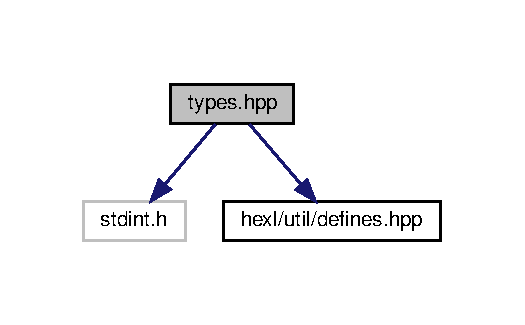
\includegraphics[width=268pt]{types_8hpp__incl}
\end{center}
\end{figure}
This graph shows which files directly or indirectly include this file\+:
\nopagebreak
\begin{figure}[H]
\begin{center}
\leavevmode
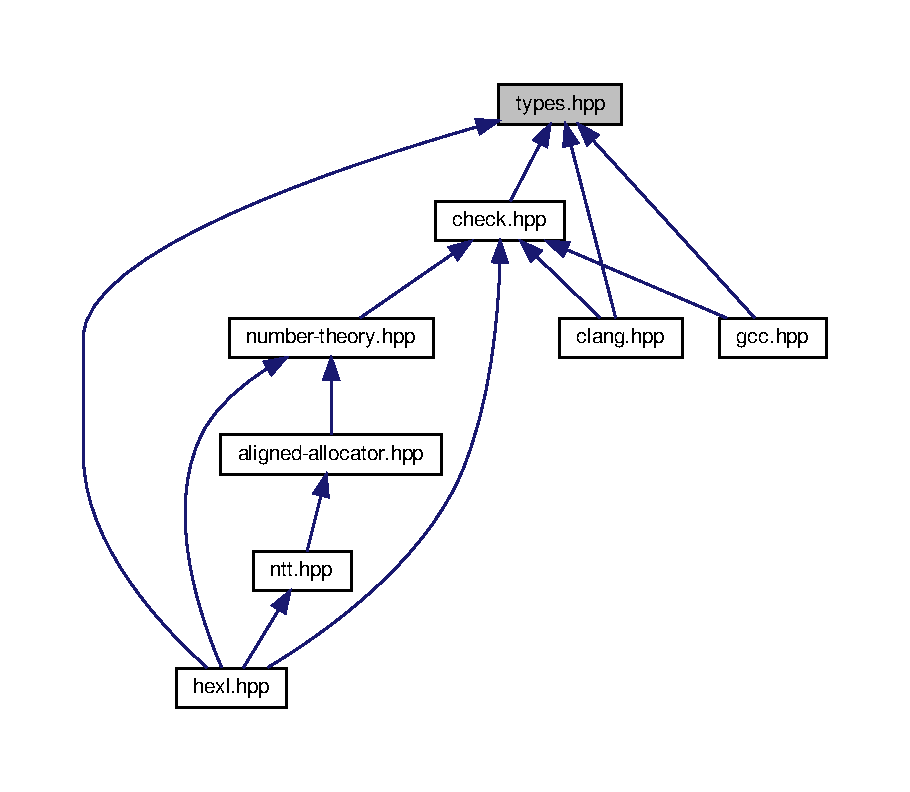
\includegraphics[width=350pt]{types_8hpp__dep__incl}
\end{center}
\end{figure}

\hypertarget{util_8hpp}{}\doxysection{util.\+hpp File Reference}
\label{util_8hpp}\index{util.hpp@{util.hpp}}
{\ttfamily \#include $<$cstddef$>$}\newline
Include dependency graph for util.\+hpp\+:
\nopagebreak
\begin{figure}[H]
\begin{center}
\leavevmode
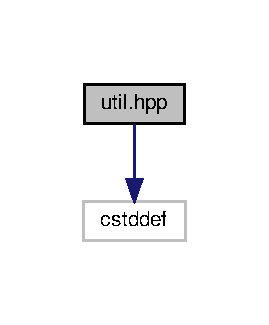
\includegraphics[width=133pt]{util_8hpp__incl}
\end{center}
\end{figure}
This graph shows which files directly or indirectly include this file\+:
\nopagebreak
\begin{figure}[H]
\begin{center}
\leavevmode
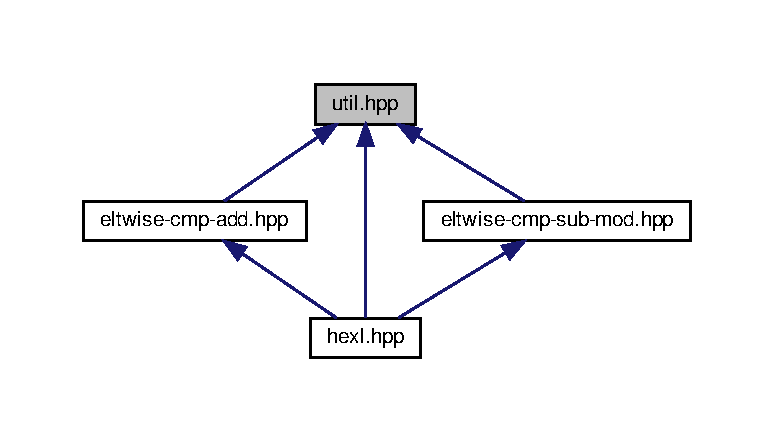
\includegraphics[width=350pt]{util_8hpp__dep__incl}
\end{center}
\end{figure}
\doxysubsection*{Namespaces}
\begin{DoxyCompactItemize}
\item 
 \mbox{\hyperlink{namespaceintel}{intel}}
\item 
 \mbox{\hyperlink{namespaceintel_1_1hexl}{intel\+::hexl}}
\end{DoxyCompactItemize}
\doxysubsection*{Enumerations}
\begin{DoxyCompactItemize}
\item 
enum \mbox{\hyperlink{namespaceintel_1_1hexl_abdcc9d2d5bb10fa95d5f143874508006}{intel\+::hexl\+::\+C\+M\+P\+I\+NT}} \{ \newline
\mbox{\hyperlink{namespaceintel_1_1hexl_abdcc9d2d5bb10fa95d5f143874508006a2dcbad7477fd40561e8b8198f173bd47}{intel\+::hexl\+::\+C\+M\+P\+I\+N\+T\+::\+EQ}} = 0, 
\mbox{\hyperlink{namespaceintel_1_1hexl_abdcc9d2d5bb10fa95d5f143874508006ac562607189d77eb9dfb707464c1e7b0b}{intel\+::hexl\+::\+C\+M\+P\+I\+N\+T\+::\+LT}} = 1, 
\mbox{\hyperlink{namespaceintel_1_1hexl_abdcc9d2d5bb10fa95d5f143874508006acfe6055d2e0503be378bb63449ec7ba6}{intel\+::hexl\+::\+C\+M\+P\+I\+N\+T\+::\+LE}} = 2, 
\mbox{\hyperlink{namespaceintel_1_1hexl_abdcc9d2d5bb10fa95d5f143874508006a946003f97ccc52d5d3b54ac0ec31bbfc}{intel\+::hexl\+::\+C\+M\+P\+I\+N\+T\+::\+F\+A\+L\+SE}} = 3, 
\newline
\mbox{\hyperlink{namespaceintel_1_1hexl_abdcc9d2d5bb10fa95d5f143874508006adc33066c3993e0d50896e533fd692ce0}{intel\+::hexl\+::\+C\+M\+P\+I\+N\+T\+::\+NE}} = 4, 
\mbox{\hyperlink{namespaceintel_1_1hexl_abdcc9d2d5bb10fa95d5f143874508006ad7d6a13c7b311ec8a3c9fcfb1919a2f8}{intel\+::hexl\+::\+C\+M\+P\+I\+N\+T\+::\+N\+LT}} = 5, 
\mbox{\hyperlink{namespaceintel_1_1hexl_abdcc9d2d5bb10fa95d5f143874508006aacd748f300c5d189c47807e2a9d6ea57}{intel\+::hexl\+::\+C\+M\+P\+I\+N\+T\+::\+N\+LE}} = 6, 
\mbox{\hyperlink{namespaceintel_1_1hexl_abdcc9d2d5bb10fa95d5f143874508006ac0d83f0b82a6b30de8811e69e6d95c61}{intel\+::hexl\+::\+C\+M\+P\+I\+N\+T\+::\+T\+R\+UE}} = 7
 \}
\begin{DoxyCompactList}\small\item\em Represents binary operations between two boolean values. \end{DoxyCompactList}\end{DoxyCompactItemize}
\doxysubsection*{Functions}
\begin{DoxyCompactItemize}
\item 
C\+M\+P\+I\+NT \mbox{\hyperlink{namespaceintel_1_1hexl_a8c654502a5e7fe2cfdd198f0fd920f2a}{intel\+::hexl\+::\+Not}} (C\+M\+P\+I\+NT cmp)
\begin{DoxyCompactList}\small\item\em Returns the logical negation of a binary operation. \end{DoxyCompactList}\end{DoxyCompactItemize}

%--- End generated contents ---

% Index
\backmatter
\newpage
\phantomsection
\clearemptydoublepage
\addcontentsline{toc}{chapter}{Index}
\printindex

\end{document}
